\documentclass[11pt]{article}

\usepackage{graphicx}

\usepackage{amsmath}

\usepackage{hyperref}
\usepackage{subcaption}
\usepackage{geometry}
\usepackage{listings}
\usepackage{xcolor}
\geometry{margin=1in}

\title{\textbf{Federated Learning: Adaptive Strategies and Performance Evaluation}}

\author{Introduction to Automated Driving -- Practical Project\\Team Federated Learning}

\date{June 2025}

\begin{document}

    \maketitle

    \section{Introduction}

    In the modern landscape of artificial intelligence and edge computing, Federated Learning (FL) has emerged as a pivotal technique to enable collaborative machine learning while preserving data privacy~\cite{rahman2021challenges}. Traditional machine learning workflows often rely on centralized data collection, where all training data must be aggregated into a single location~\cite{mcmahan2017communication}. This approach, while effective in many domains, poses significant challenges in terms of privacy, data security, and regulatory compliance, especially when dealing with sensitive or distributed data sources such as mobile devices, autonomous vehicles, or healthcare systems~\cite{chai2024survey}.

    Federated Learning redefines this paradigm by distributing the model training process across multiple devices or clients, each of which retains its local data. Rather than transmitting raw data to a central server, clients perform local training and share only model updates (e.g., gradients or weights). These updates are then aggregated by a central server to improve the global model. This decentralized approach not only reduces privacy risks but also minimizes communication costs and enables learning from previously inaccessible data~\cite{mcmahan2017communication}.

    This approach is particularly valuable in domains like automated driving, where vehicles generate massive volumes of sensor and image data that are both privacy-sensitive and bandwidth-intensive to transmit. In such scenarios, FL enables vehicles to learn collaboratively from diverse driving experiences across regions, conditions, and users—without ever sharing raw sensor data. This makes FL a powerful enabler for scalable and privacy-preserving advancements in perception, decision-making, and autonomous control systems~\cite{rahman2021challenges}.

    \subsection{Problem Statement}

    This project addresses two key challenges in federated learning:

    \subsubsection{Evaluating Base Federated Learning Strategies on Different Partitions}
    We aim to evaluate the performance of adaptive optimization techniques in federated learning settings.
    The core objective is to analyze how strategies such as FedAvg and Adaptive Federated Optimization (FedOpt) perform under different data distribution scenarios, particularly in non-IID environments.
    This comparison is essential to identify methods that generalize well while maintaining computational efficiency and privacy.

    \subsubsection{Minimizing Round Timeouts in Full Participation Settings}
    In the second experiment, we investigate the challenges associated with full client participation (\texttt{fraction\_fit = 1.0}), where all clients take part in every training round. This configuration ensures maximal resource utilization and consistent participation, but it also introduces the risk of some slower clients dictating the round duration.

    To better reflect real-world heterogeneity, we simulate scenarios where clients differ in computational resources (e.g. CPU vs. GPU) and local training effort. Clients train independently, and the server synchronizes updates after a fixed interval, simulating a semi-asynchronous training process.
    The objective here is to assess how adaptive optimization techniques can help mitigate the impact of slow clients and reduce timeout risks, ensuring efficient and stable convergence even in challenging deployment environments.
    This pipeline will be tested using the previously mentioned FedAvg and Adaptive Federated Optimization, but also using a novel federated aggregation technique (FedAvg-Weighted) which, in addition to aggregating the weights based on the number of samples each client had, it also takes into consideration the number of epochs did on that specific client.


    \section{Algorithms}

    \subsection{FedAvg}
    \label{subsec:fedavg}

    Federated Averaging (FedAvg) is a widely-used baseline in FL. Each client performs local training on its data, and the server aggregates the model updates using a weighted average.

    \textbf{Pseudocode: FedAvg}

    \begin{enumerate}
        \item Initialize global model weights $w_0$
        \item For each round $t=1,2,\dots,T$:
        \begin{enumerate}
            \item Server sends $w_t$ to selected clients
            \item Each client $k$ updates $w_t$ to $w_{t+1}^k$ via local SGD
            \item Server aggregates updates: $w_{t+1} = \sum_k \frac{n_k}{n} w_{t+1}^k$
        \end{enumerate}
    \end{enumerate}

    \subsection{Adaptive Federated Optimization (FedOpt)}
    \label{subsec:fedopt}

    We implemented the Adaptive Federated Optimization strategy proposed by Reddi et al. \cite{Reddi2020AdaptiveFO}, which extends FedAvg with adaptive optimization methods (AdaGrad, Adam, Yogi) at the server level. Adaptive Federated Optimization introduces federated versions of adaptive optimizers like Adagrad, Adam, and Yogi to address challenges in federated learning, particularly data heterogeneity and communication efficiency. By integrating these adaptive methods, the approach enhances convergence and performance over traditional methods like FedAvg, especially in non-convex settings with diverse client data. The \textbf{pseudocode} for this approach can be seen in Figure \ref{fig:fedopt_alg}.

    \begin{figure}[h!]
        \centering
        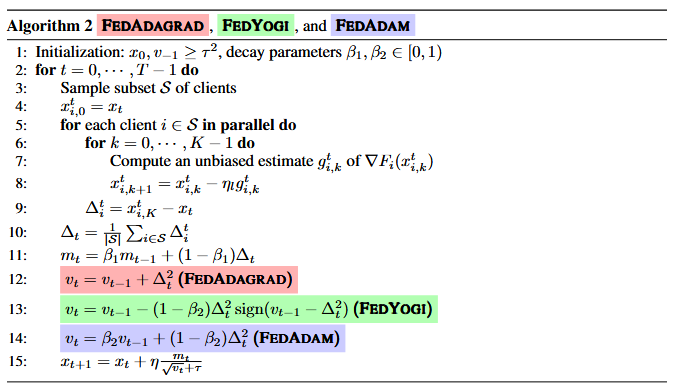
\includegraphics[width=0.9\textwidth]{img/fedopt_alg}
        \caption{Pseudocode for Adaptive Federated Optimization}
        \label{fig:fedopt_alg}
    \end{figure}

    \vspace{200pt}

    \subsection{Weighted-FedAvg}
    This algorithm has the same idea as FedAvg (Section \ref{subsec:fedavg}), but all the clients are chosen for training (instead of few of them), the clients train for different number of epochs and, in the aggregation step, the weights are scaled based on both the number of samples and the number of epochs the local weights were trained on.

    \textbf{Pseudocode: Weighted-FedAvg}

    \begin{enumerate}
        \item Initialize global model weights $w_0$
        \item For each round $t=1,2,\dots,T$:
        \begin{enumerate}
            \item Server sends $w_t$ to \textbf{all} clients
            \item Each client $k$ updates $w_t$ to $w_{t+1}^k$ via local SGD on the local data ($n_k$ samples) and on a various number of epochs ($e_k$).
            \item Server aggregates updates: $w_{t+1} = \sum_k \frac{n_k \cdot e_k}{\sum_j n_j \cdot e_j} w_{t+1}^k$
        \end{enumerate}
    \end{enumerate}


    \section{Experimental Setup}

    \subsection{Task and Dataset}

    We selected the CIFAR-10 dataset \cite{krizhevsky2009learning} for our image classification task. CIFAR-10 is a benchmark dataset consisting of \textbf{60,000 32x32 color images} in \textbf{10 different classes}, with 6,000 images per class.

    Figure~\ref{fig:cifar10} shows example images from each class.

    \begin{figure}[h]
        \centering
        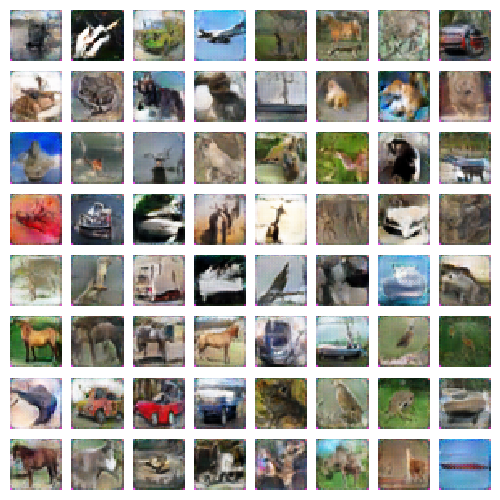
\includegraphics[width=0.5\textwidth]{img/cifar10_samples}
        \caption{Sample images from the CIFAR-10 dataset.}
        \label{fig:cifar10}
    \end{figure}

    To perform the classification task, we employed the \textbf{VGG-11} architecture \cite{Simonyan2014VeryDC}, a convolutional neural network (CNN) developed by the Visual Geometry Group at the University of Oxford.
    VGG-11 consists of 11 layers: 8 convolutional layers followed by 3 fully connected layers.
    It is known for its simplicity and effectiveness in image recognition tasks.

    The model was trained under both centralized and federated learning setups.
    In both cases, we implemented the model using PyTorch, and for the federated learning setup, we used the Flower framework \cite{beutel2020flower} to simulate multiple clients.

    Figure~\ref{fig:vgg11} provides a high-level overview of the VGG-11 architecture.

    \begin{figure}[h]
        \centering
        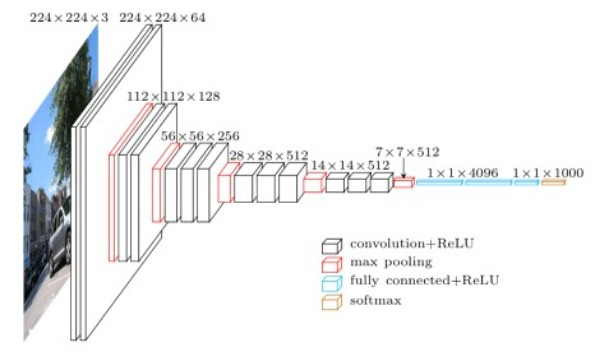
\includegraphics[width=0.75\textwidth]{img/vgg11_diagram}
        \caption{VGG-11 architecture used for image classification.}
        \label{fig:vgg11}
    \end{figure}

    \subsection{Partitioning Strategies}
    \label{subsec:partitioning}

    To simulate a variety of realistic and synthetic data heterogeneity scenarios in federated learning, we implemented several data partitioning strategies. (examples in Figure~\ref{fig:partitioning_2x2})

    \begin{itemize}
        \item \textbf{IID} – uniform, randomly sampled data distribution.
        \item \textbf{Dirichlet} – label distributions drawn from a Dirichlet distribution with configurable concentration parameter.
        \item \textbf{Pathological} – each client receives data from a limited number of classes (e.g., two).
        \item \textbf{Shard} – data is sorted by label and divided into shards, with each client receiving a few shards.
        \item \textbf{Size} – clients are assigned partitions of configurable sizes.
        \item \textbf{Linear, Square, Exponential} – variations that assign partition sizes based on linear, squared, or exponential proportions.
    \end{itemize}

    \begin{figure}[h]
        \centering

        \begin{subfigure}[b]{0.45\textwidth}
            \centering
            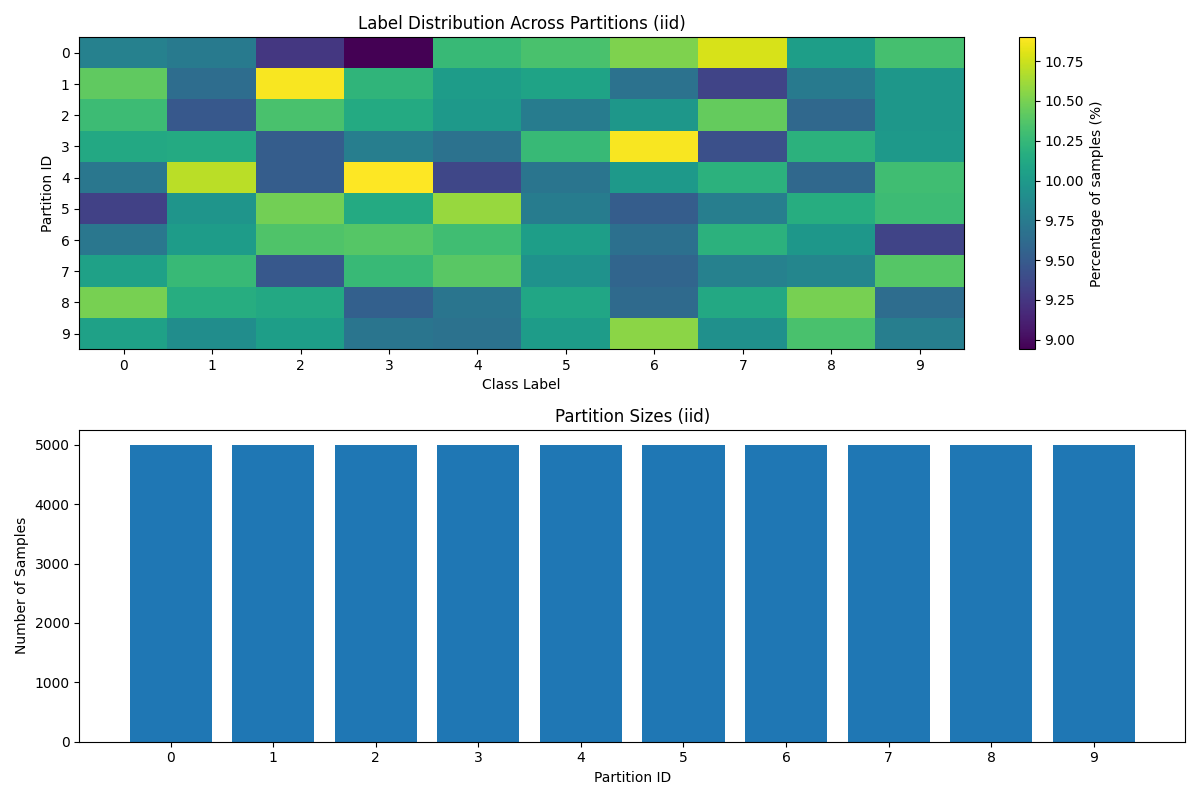
\includegraphics[width=\textwidth]{img/partitions/partition_distribution_iid}
            \caption{IID Partitioning}
            \label{fig:iid_partitioning}
        \end{subfigure}
        \hfill
        \begin{subfigure}[b]{0.45\textwidth}
            \centering
            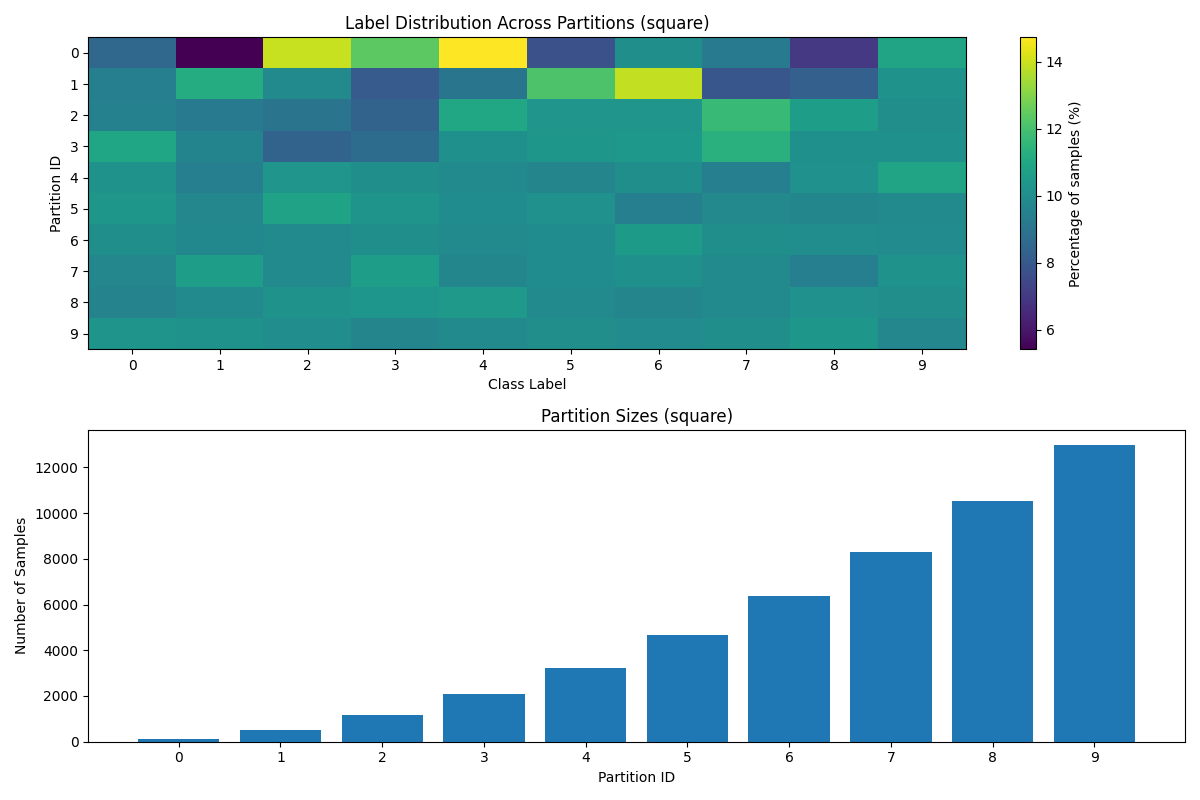
\includegraphics[width=\textwidth]{img/partitions/partition_distribution_square}
            \caption{Square Partitioning}
            \label{fig:square_partitioning}
        \end{subfigure}

        \vspace{0.5cm}

        \begin{subfigure}[b]{0.45\textwidth}
            \centering
            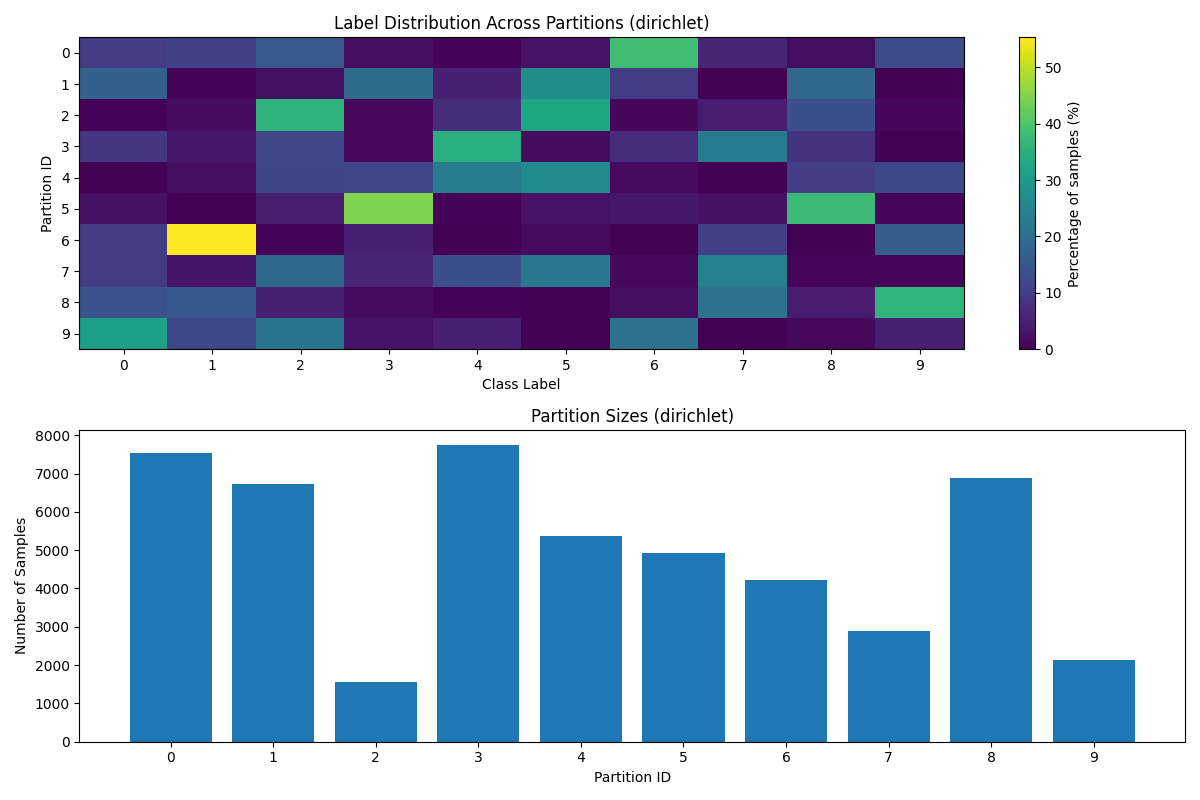
\includegraphics[width=\textwidth]{img/partitions/partition_distribution_dirichlet}
            \caption{Dirichlet partitioning}
            \label{fig:dirichlet_partitioning}
        \end{subfigure}
        \hfill
        \begin{subfigure}[b]{0.45\textwidth}
            \centering
            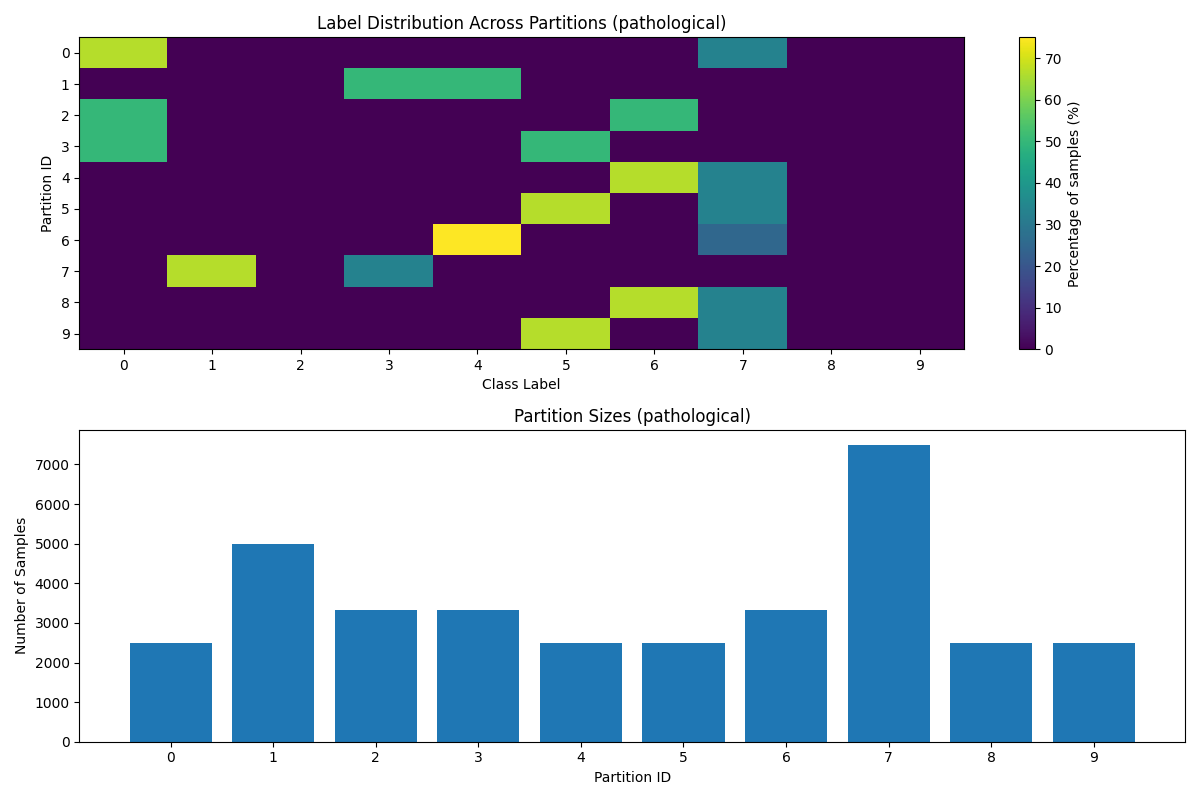
\includegraphics[width=\textwidth]{img/partitions/partition_distribution_pathological}
            \caption{Pathological partitioning}
            \label{fig:pathological_partitioning}
        \end{subfigure}

        \caption{Visualization of various data partitioning strategies in federated learning}
        \label{fig:partitioning_2x2}
    \end{figure}

    To support flexible experimentation, we designed a partitioning manager that abstracts partitioner instantiation.
    This system allows for easy switching between partitioning strategies via configuration arguments, rather than code changes.
    Additional hyperparameters (e.g., Dirichlet \(\alpha\), number of classes per partition) are passed as keyword arguments and handled internally by the manager.


    \section{Experiments and Results}

    For all experiments, the dataset was first divided into training and test sets, with 10\% of the data reserved for testing. From the training set, 20\% was further allocated for validation.

    \subsection{Baseline Performance}
    \label{subsec:baseline_results}

    To establish a centralized performance reference, we trained \textbf{VGG-11} in a nonfederated setting.

    Training was carried out on a single device using the Adam optimizer with a learning rate of 0.001, a batch size of 64, and for a total of 50 epochs.

    This centralized baseline serves as a reference point for evaluating the performance of federated learning approaches under identical model and different data conditions.

    The final performance was measured using the accuracy of the classification and cross-entropy loss in the test set and a test loss of 1.07 and a test accuracy of 74.9\% was obtained.

    Other metrics are illustrated in Figure~\ref{fig:baseline_metrics}.

    \begin{figure}[h]
        \centering
        \begin{subfigure}[b]{0.48\textwidth}
            \centering
            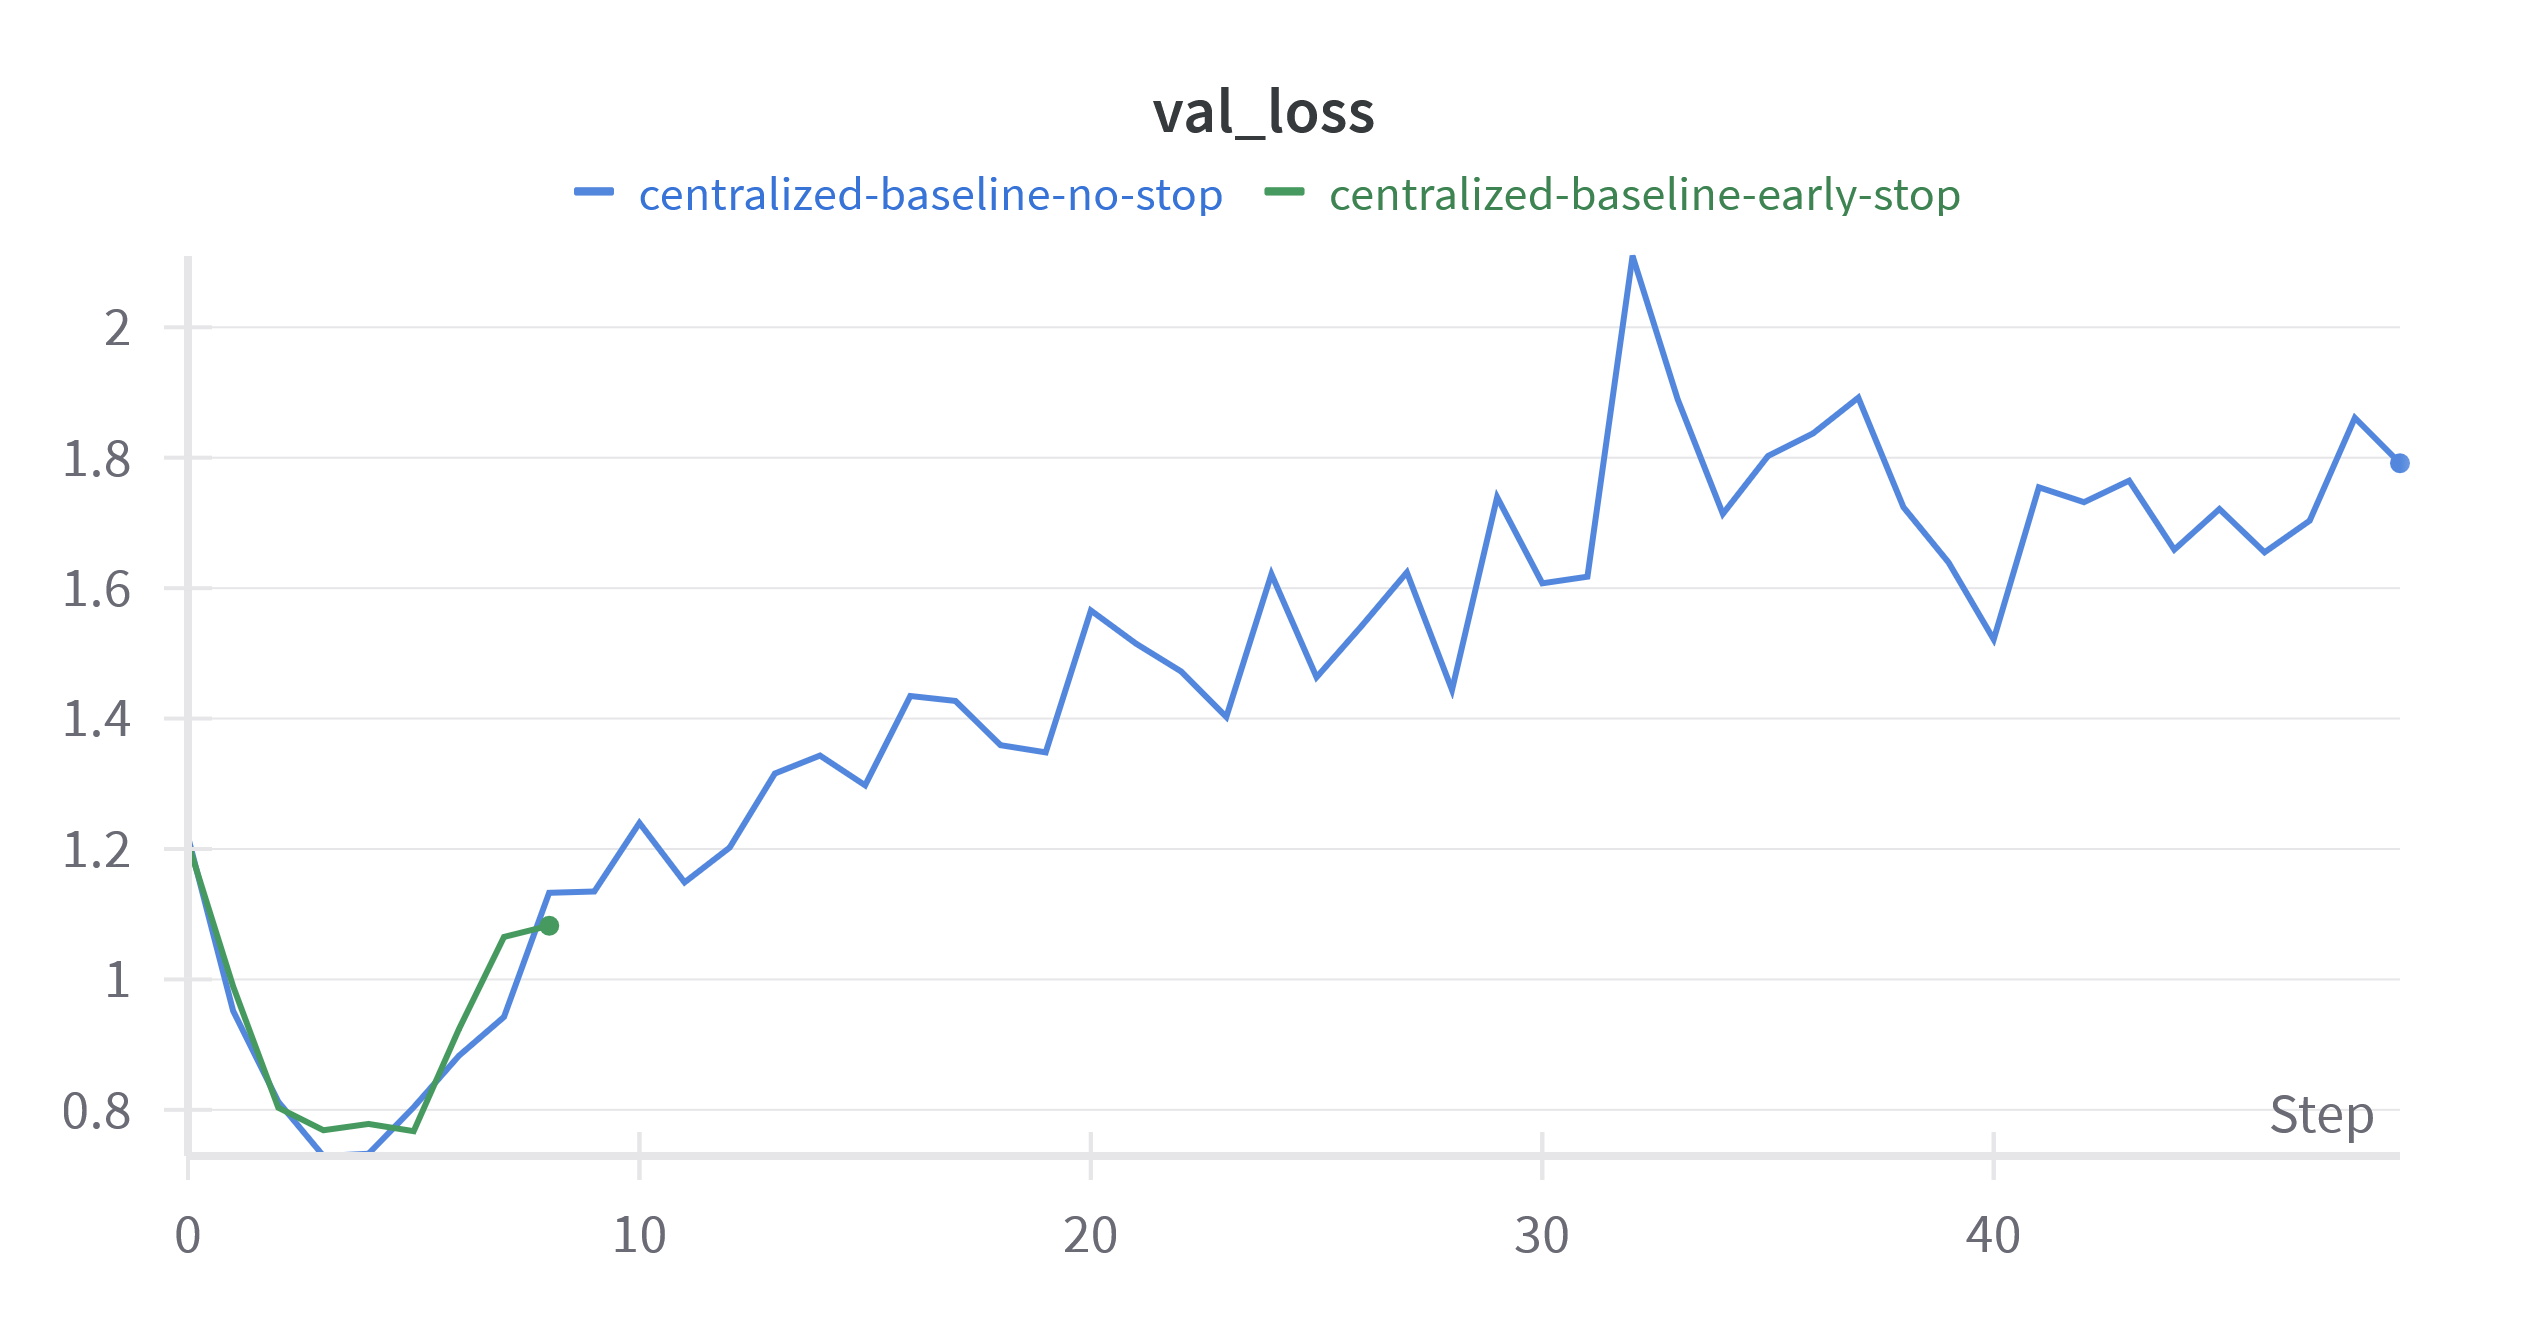
\includegraphics[width=\textwidth]{img/experiment_1/baseline_val_loss}
            \caption{Baseline val loss}
            \label{fig:baseline_val_loss}
        \end{subfigure}
        \hfill
        \begin{subfigure}[b]{0.48\textwidth}
            \centering
            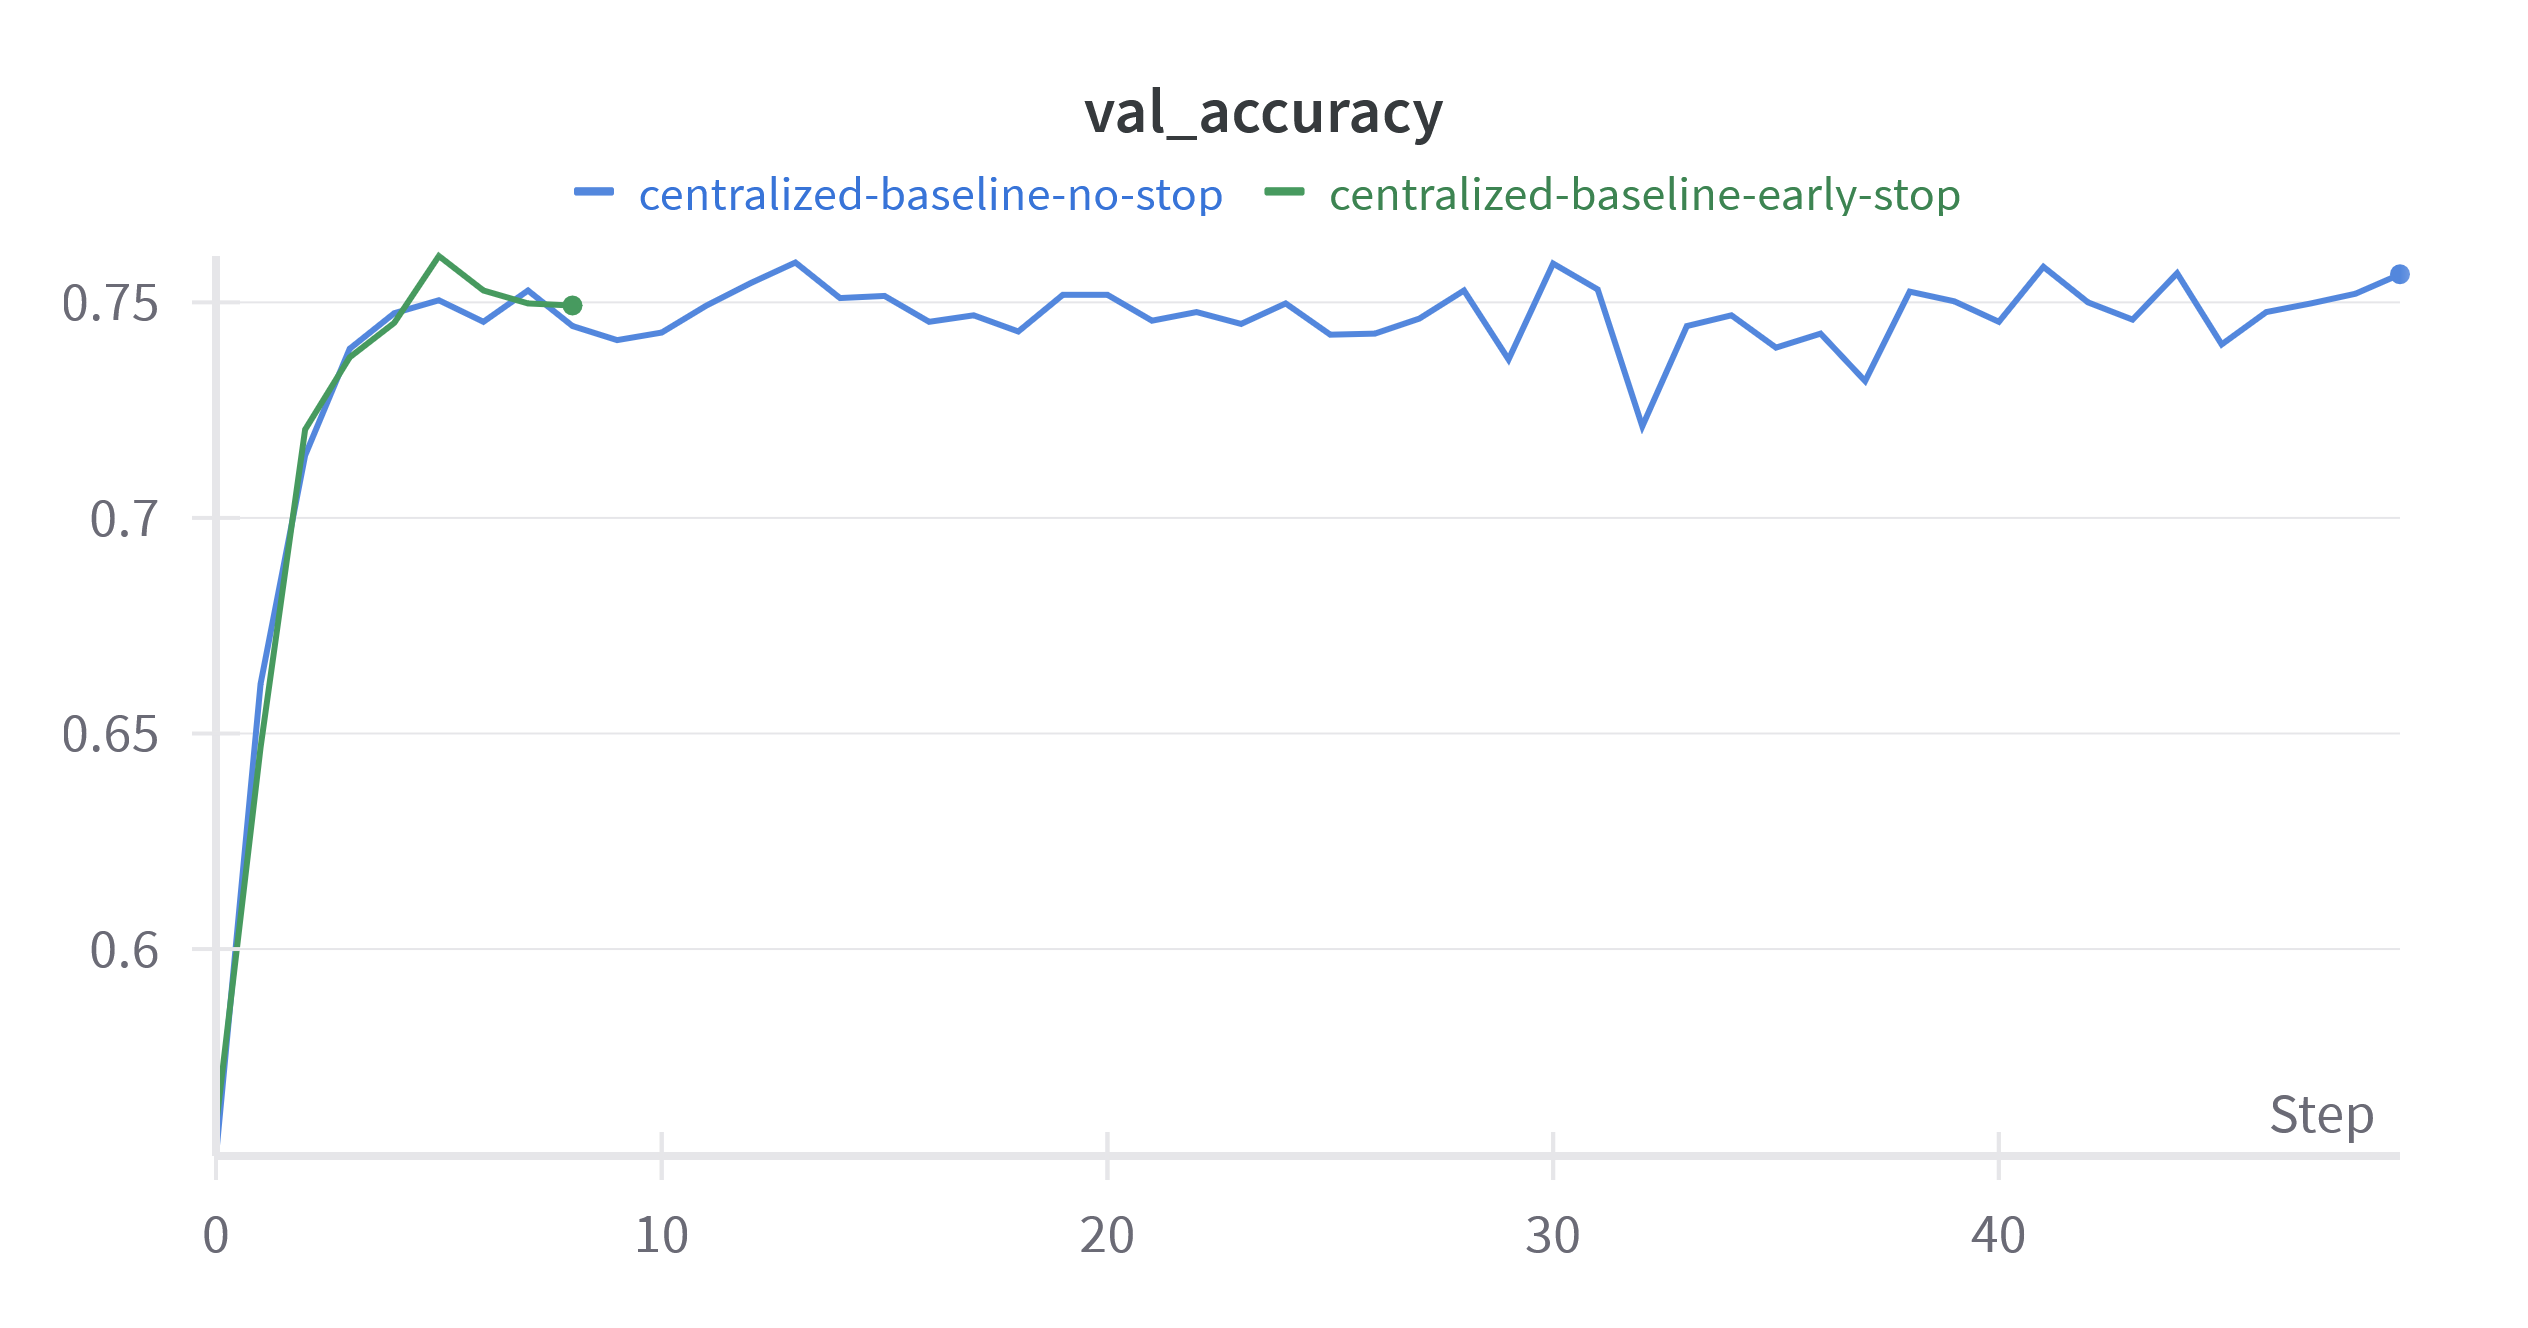
\includegraphics[width=\textwidth]{img/experiment_1/baseline_val_acc}
            \caption{Baseline val accuracy}
            \label{fig:baseline_val_acc}
        \end{subfigure}
        \caption{Baseline performance metrics evolution}
        \label{fig:baseline_metrics}
    \end{figure}

    \subsection{Experiment 1: Equal Hardware Experiment}
    \label{subsec:experiment1}

    \subsubsection{Hyperparameters}

    The following hyperparameters were used consistently across all configurations in Experiment 1, unless otherwise specified:

    \begin{itemize}
        \item \textbf{Number of clients}: 5
        \item \textbf{Number of server rounds}: 50
        \item \textbf{Fraction of clients per round}: 0.3
        \item \textbf{Server learning rate}: 0.01
        \item \textbf{Client learning rate}: 0.001
        \item \textbf{Local epochs}: 10
        \item \textbf{Batch size}: 64
        \item \textbf{Early stopping}: Enabled
        \item \textbf{Random seed}: 35
    \end{itemize}

    Optional parameters, such as the Dirichlet concentration parameter (\texttt{dirichlet-alpha = 0.5}), were used selectively depending on the scenario.

    In all runs, we assume equally capable clients with uniform compute and communication capacity. Clients train locally for a fixed number of epochs before synchronizing their updates with the central server.

    \subsubsection{Partitioning Scenarios}

    To understand the impact of data heterogeneity, we simulate the following partitioning strategies:

    \begin{itemize}
        \item \textbf{IID}: Balanced and identically distributed data across clients.
        \item \textbf{Square}: Imbalanced sample counts where the number of data points per client grows quadratically with the client index, creating significant data quantity heterogeneity.
        \item \textbf{Dirichlet}: Imbalanced data with heterogeneous class distributions, controlled by a Dirichlet prior.
    \end{itemize}

    We now present results for each of these scenarios.

    \subsubsection{IID Scenario}
    \label{subsubsec:iid-scenario}

    In the IID setup, each client receives a uniform and balanced sample from the CIFAR-10 dataset, ensuring equal representation of all classes. This configuration serves as a performance baseline and illustrates the ideal case for federated training, as shown in Figure~\ref{fig:iid_partitioning}.

    Given the simulated nature of our federated learning environment, we can evaluate comprehensive metrics including average validation and test accuracy/loss across all clients—metrics that would not be accessible in real-world federated scenarios—as well as global model performance.

    The experimental results demonstrate the comparative performance of different federated optimization strategies under IID conditions.
    Figure~\ref{fig:iid_client_metrics} shows the client-averaged validation metrics, while Figure~\ref{fig:iid_global_metrics} presents the global model performance on the test set.


    \begin{figure}[h]
        \centering
        \begin{subfigure}[b]{0.48\textwidth}
            \centering
            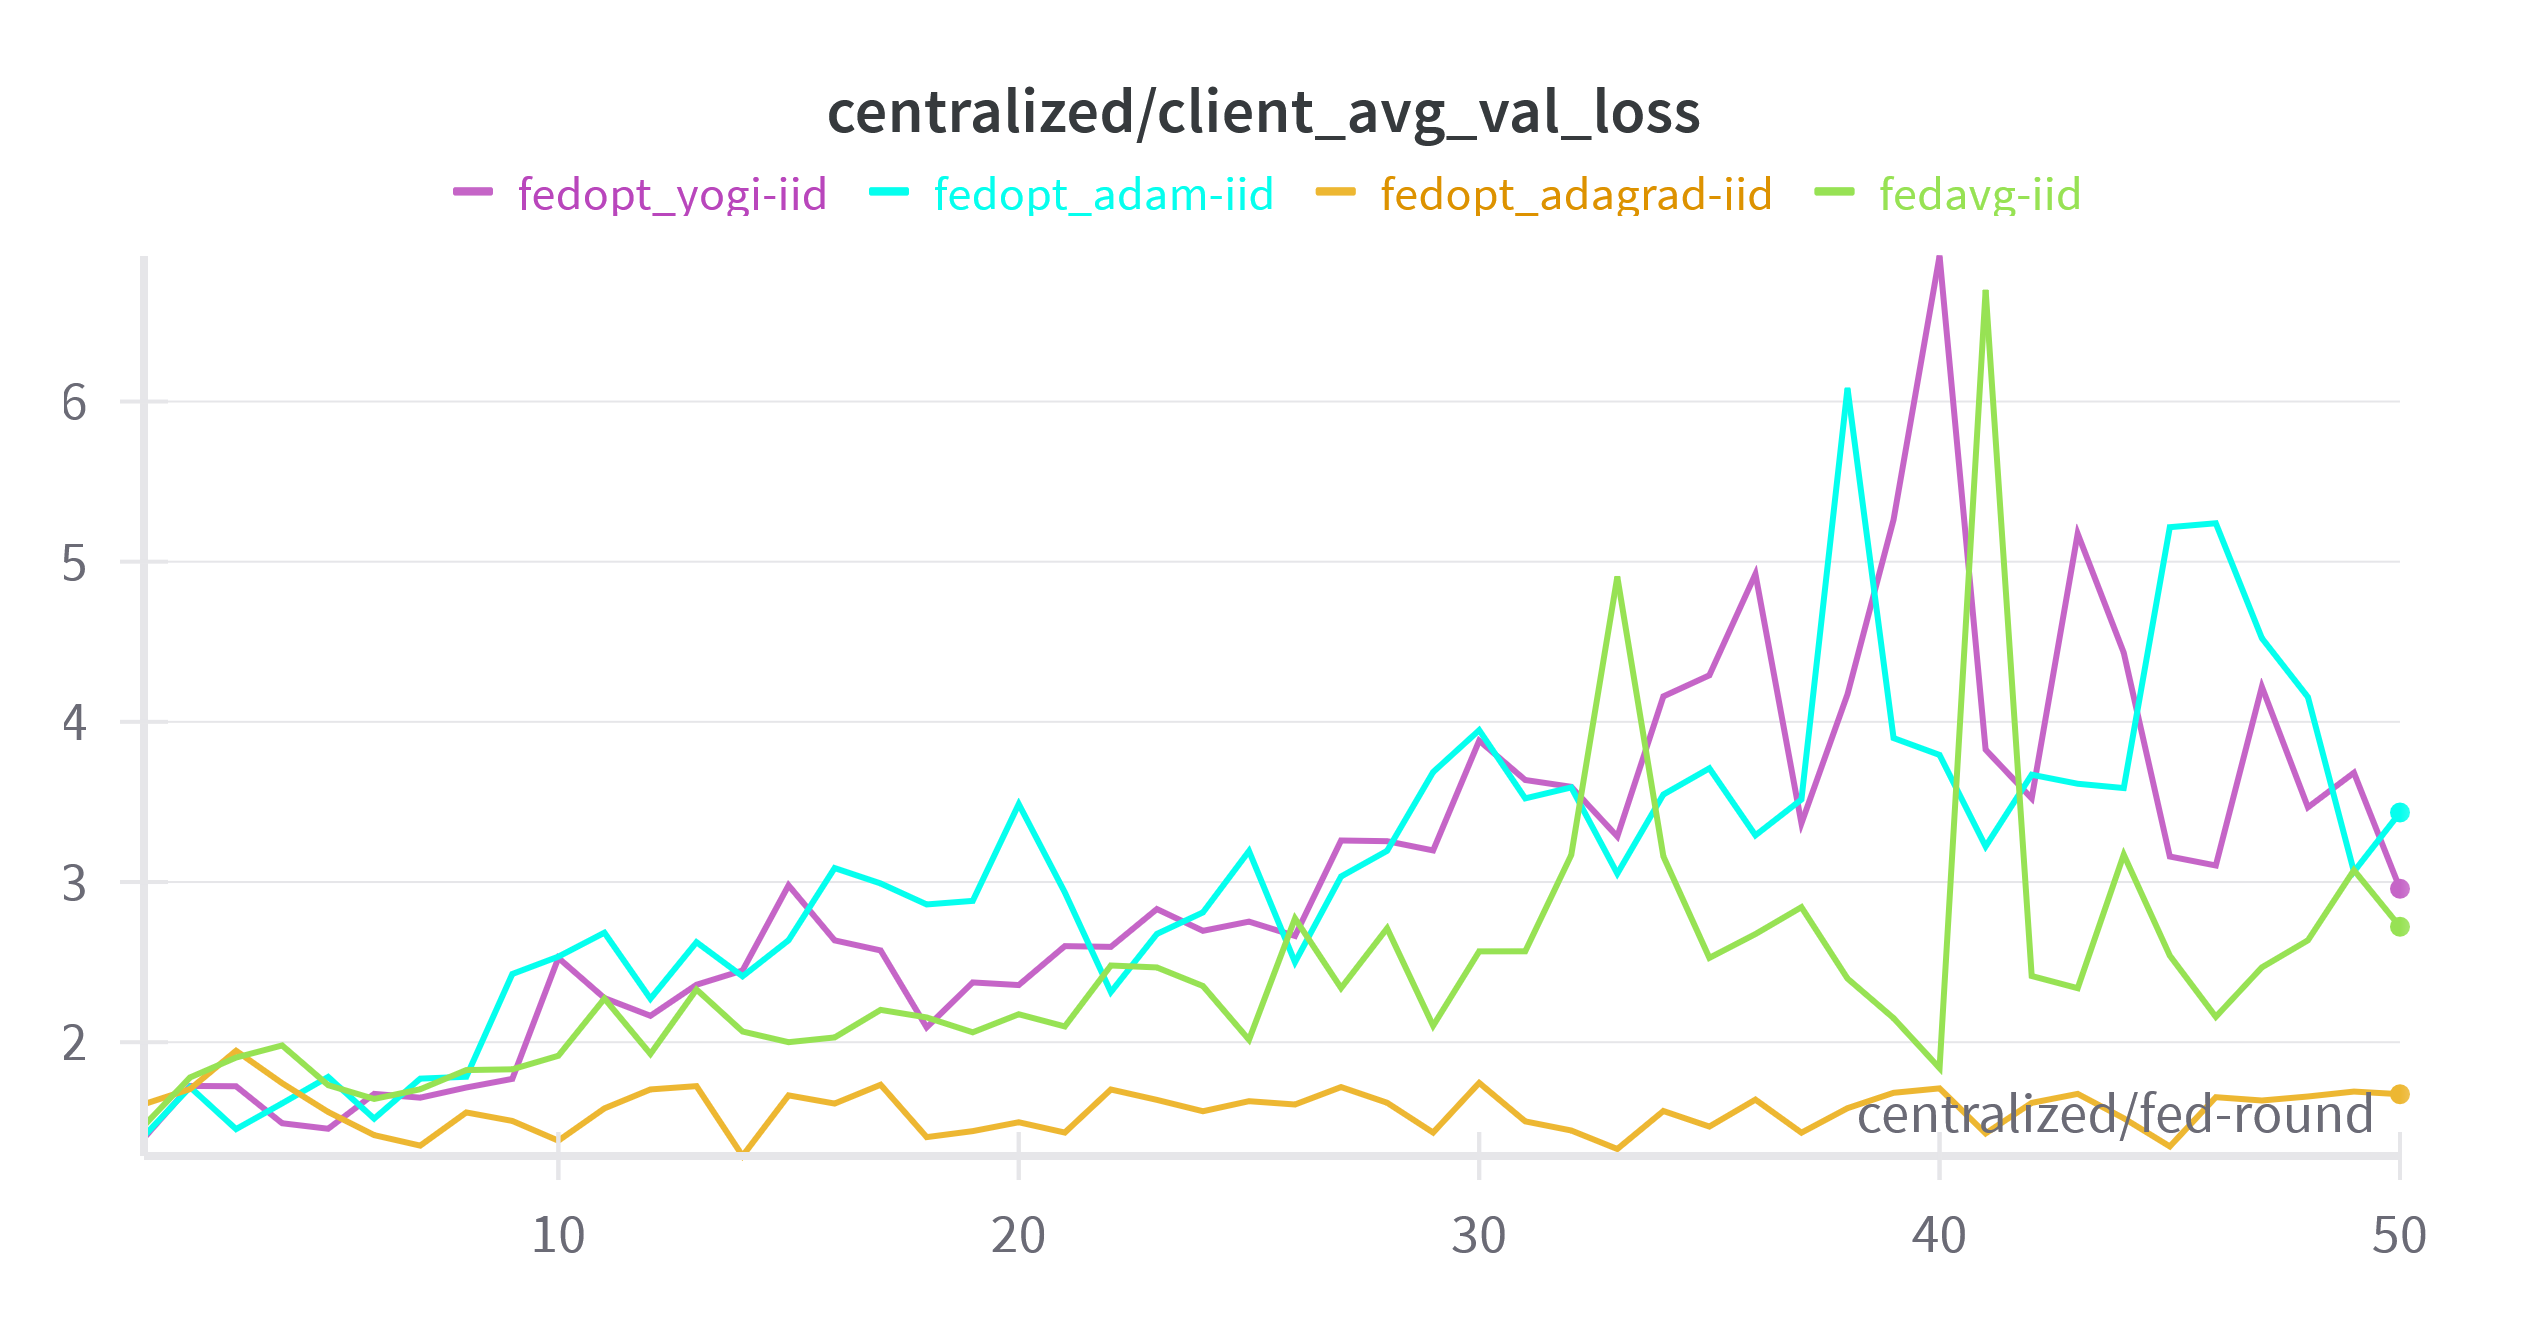
\includegraphics[width=\textwidth]{img/experiment_1/iid_client_avg_val_loss}
            \caption{Client average validation loss}
            \label{fig:iid_val_loss}
        \end{subfigure}
        \hfill
        \begin{subfigure}[b]{0.48\textwidth}
            \centering
            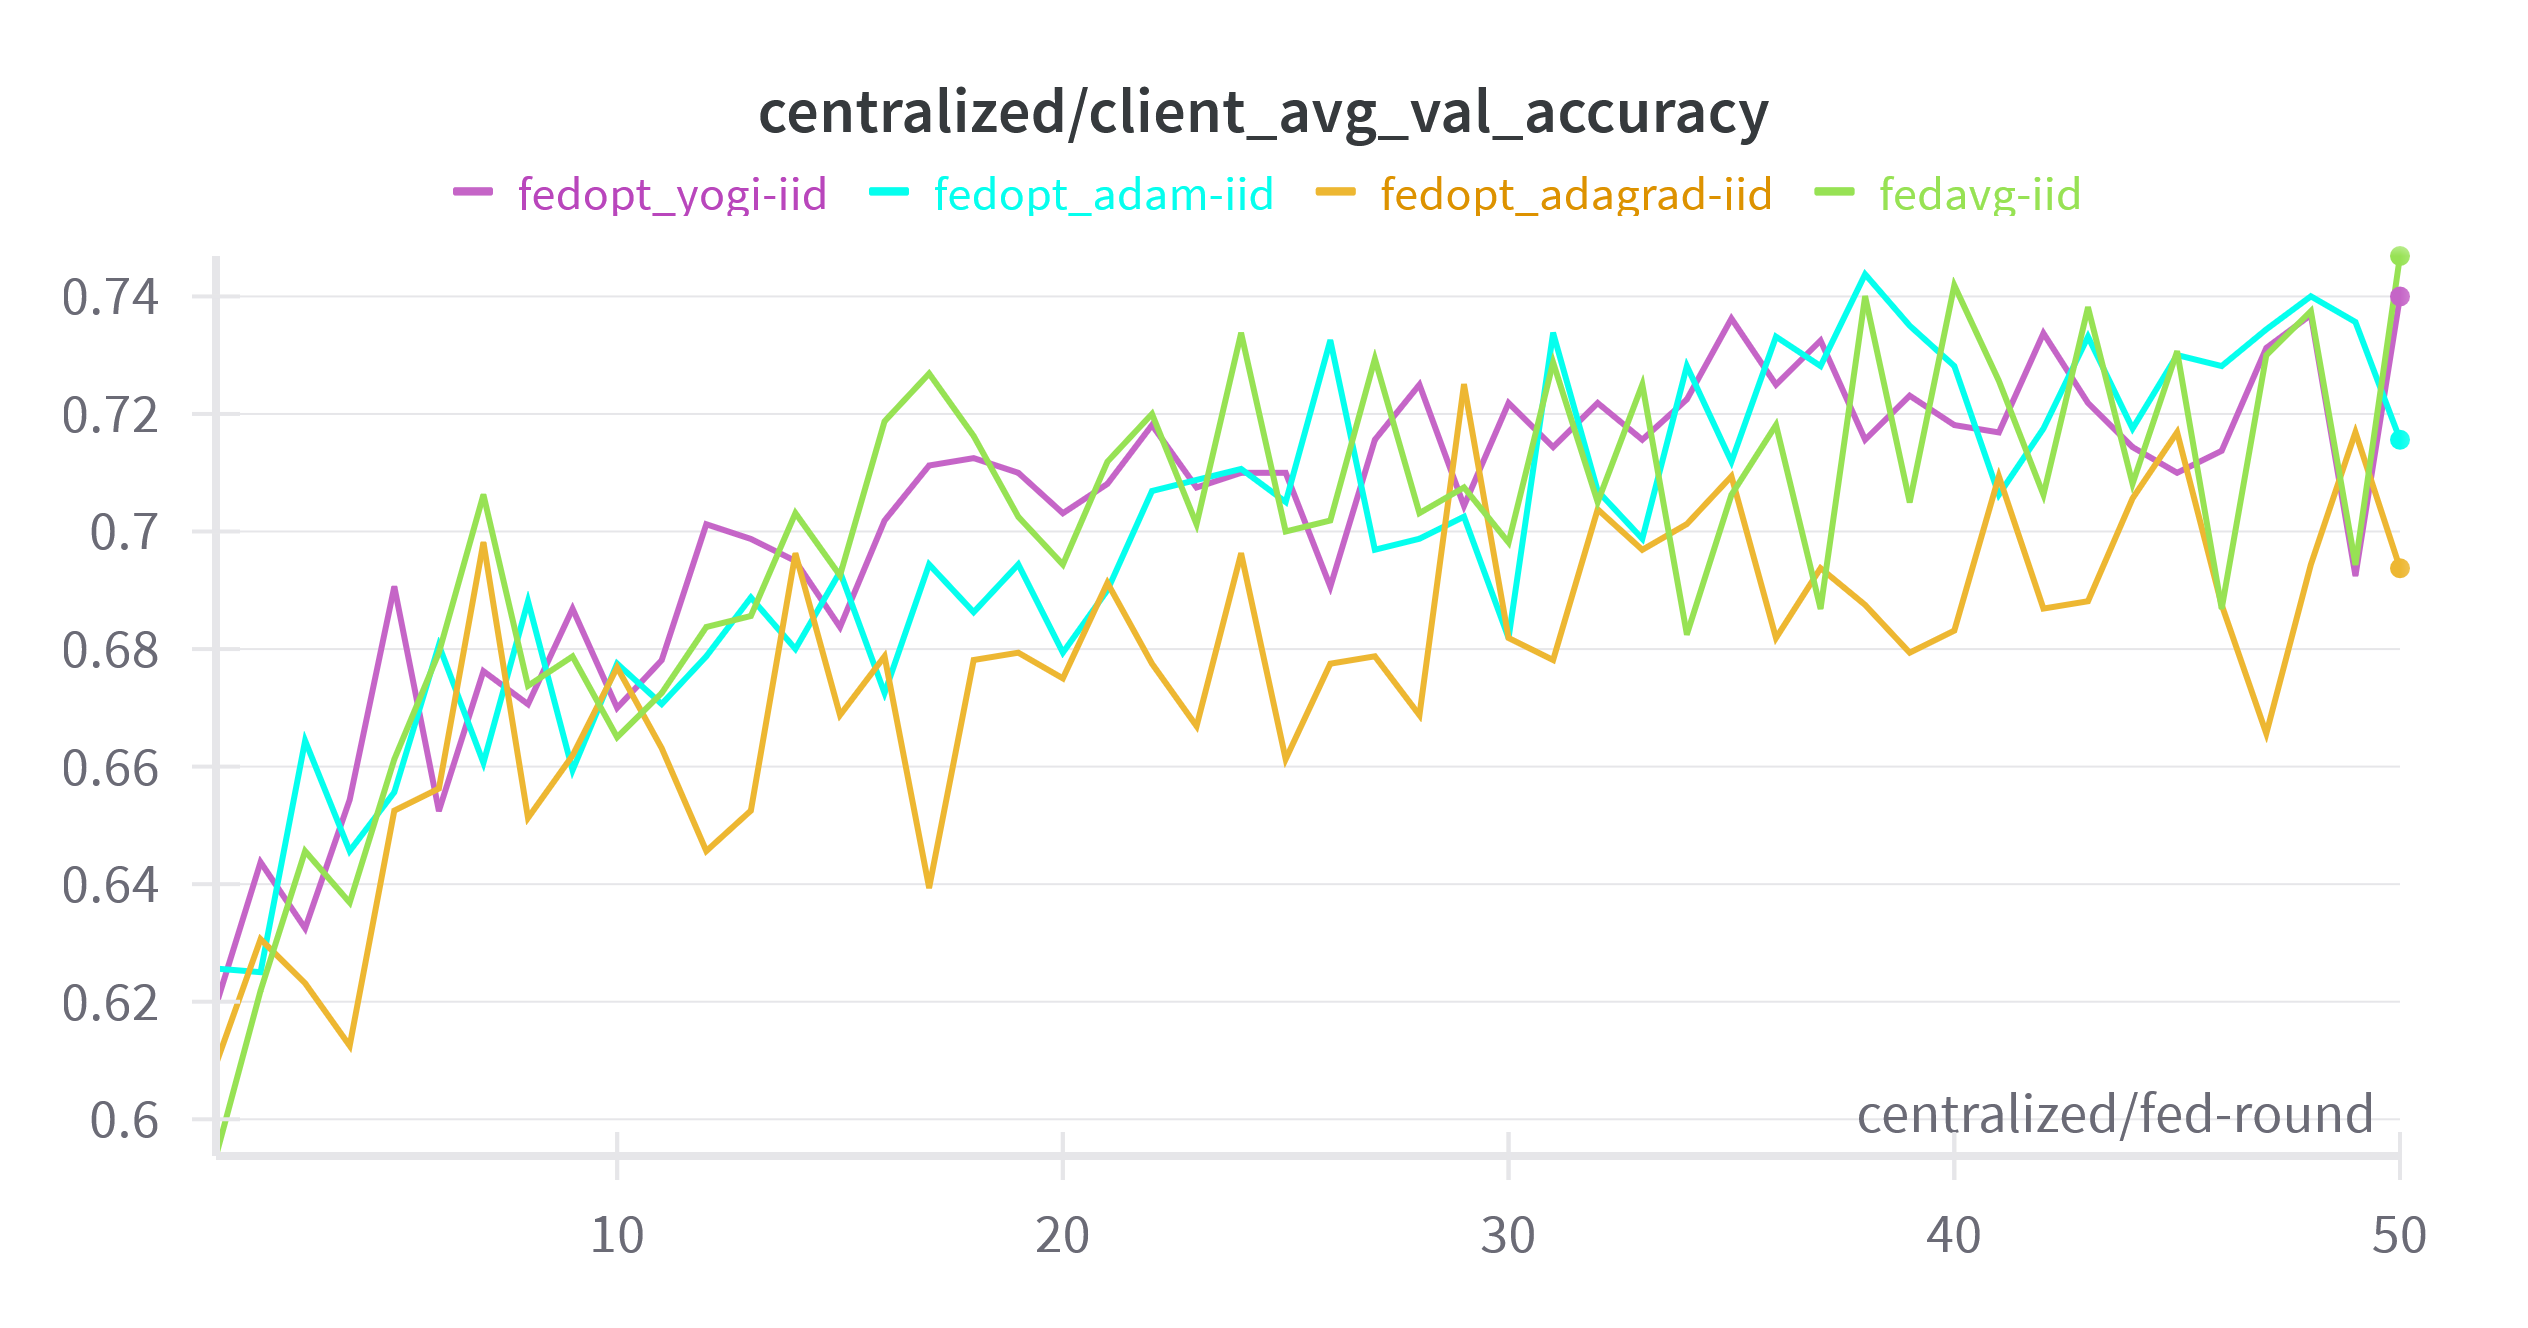
\includegraphics[width=\textwidth]{img/experiment_1/iid_client_avg_val_acc}
            \caption{Client average validation accuracy}
            \label{fig:iid_val_acc}
        \end{subfigure}
        \caption{Client-side performance metrics evolution during training for IID partitioning}
        \label{fig:iid_client_metrics}
    \end{figure}

    \begin{figure}[h]
        \centering
        \begin{subfigure}[b]{0.48\textwidth}
            \centering
            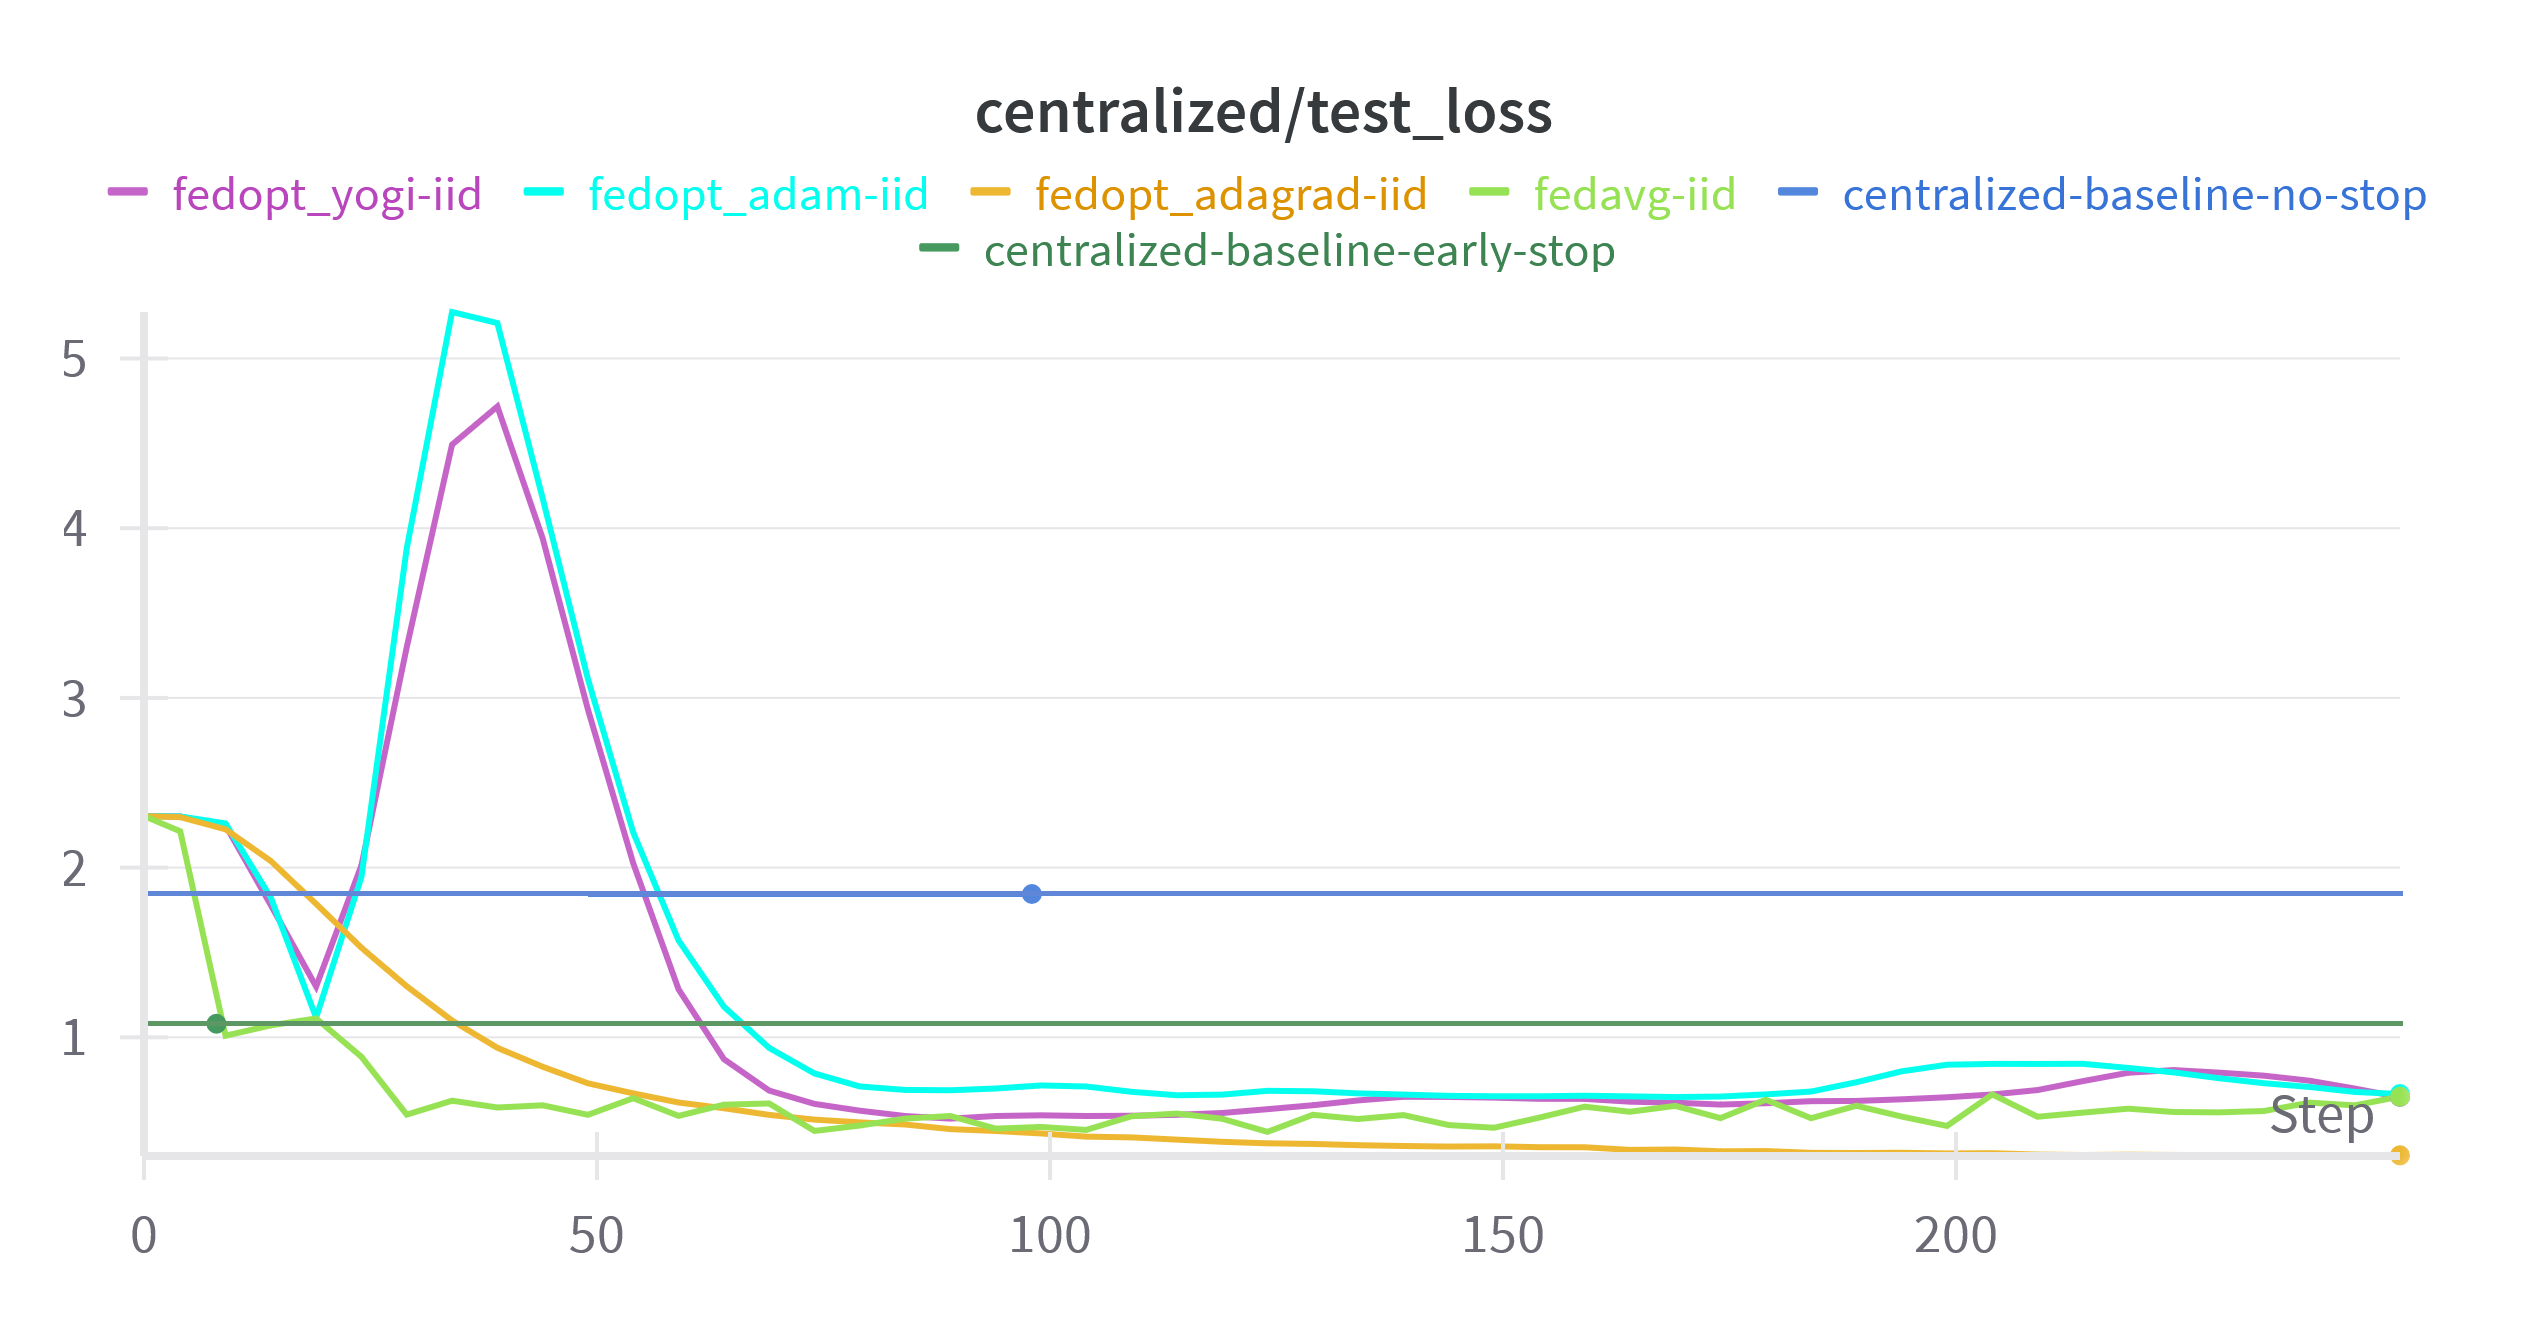
\includegraphics[width=\textwidth]{img/experiment_1/iid_server_test_loss}
            \caption{Global model test loss}
            \label{fig:iid_global_val_loss}
        \end{subfigure}
        \hfill
        \begin{subfigure}[b]{0.48\textwidth}
            \centering
            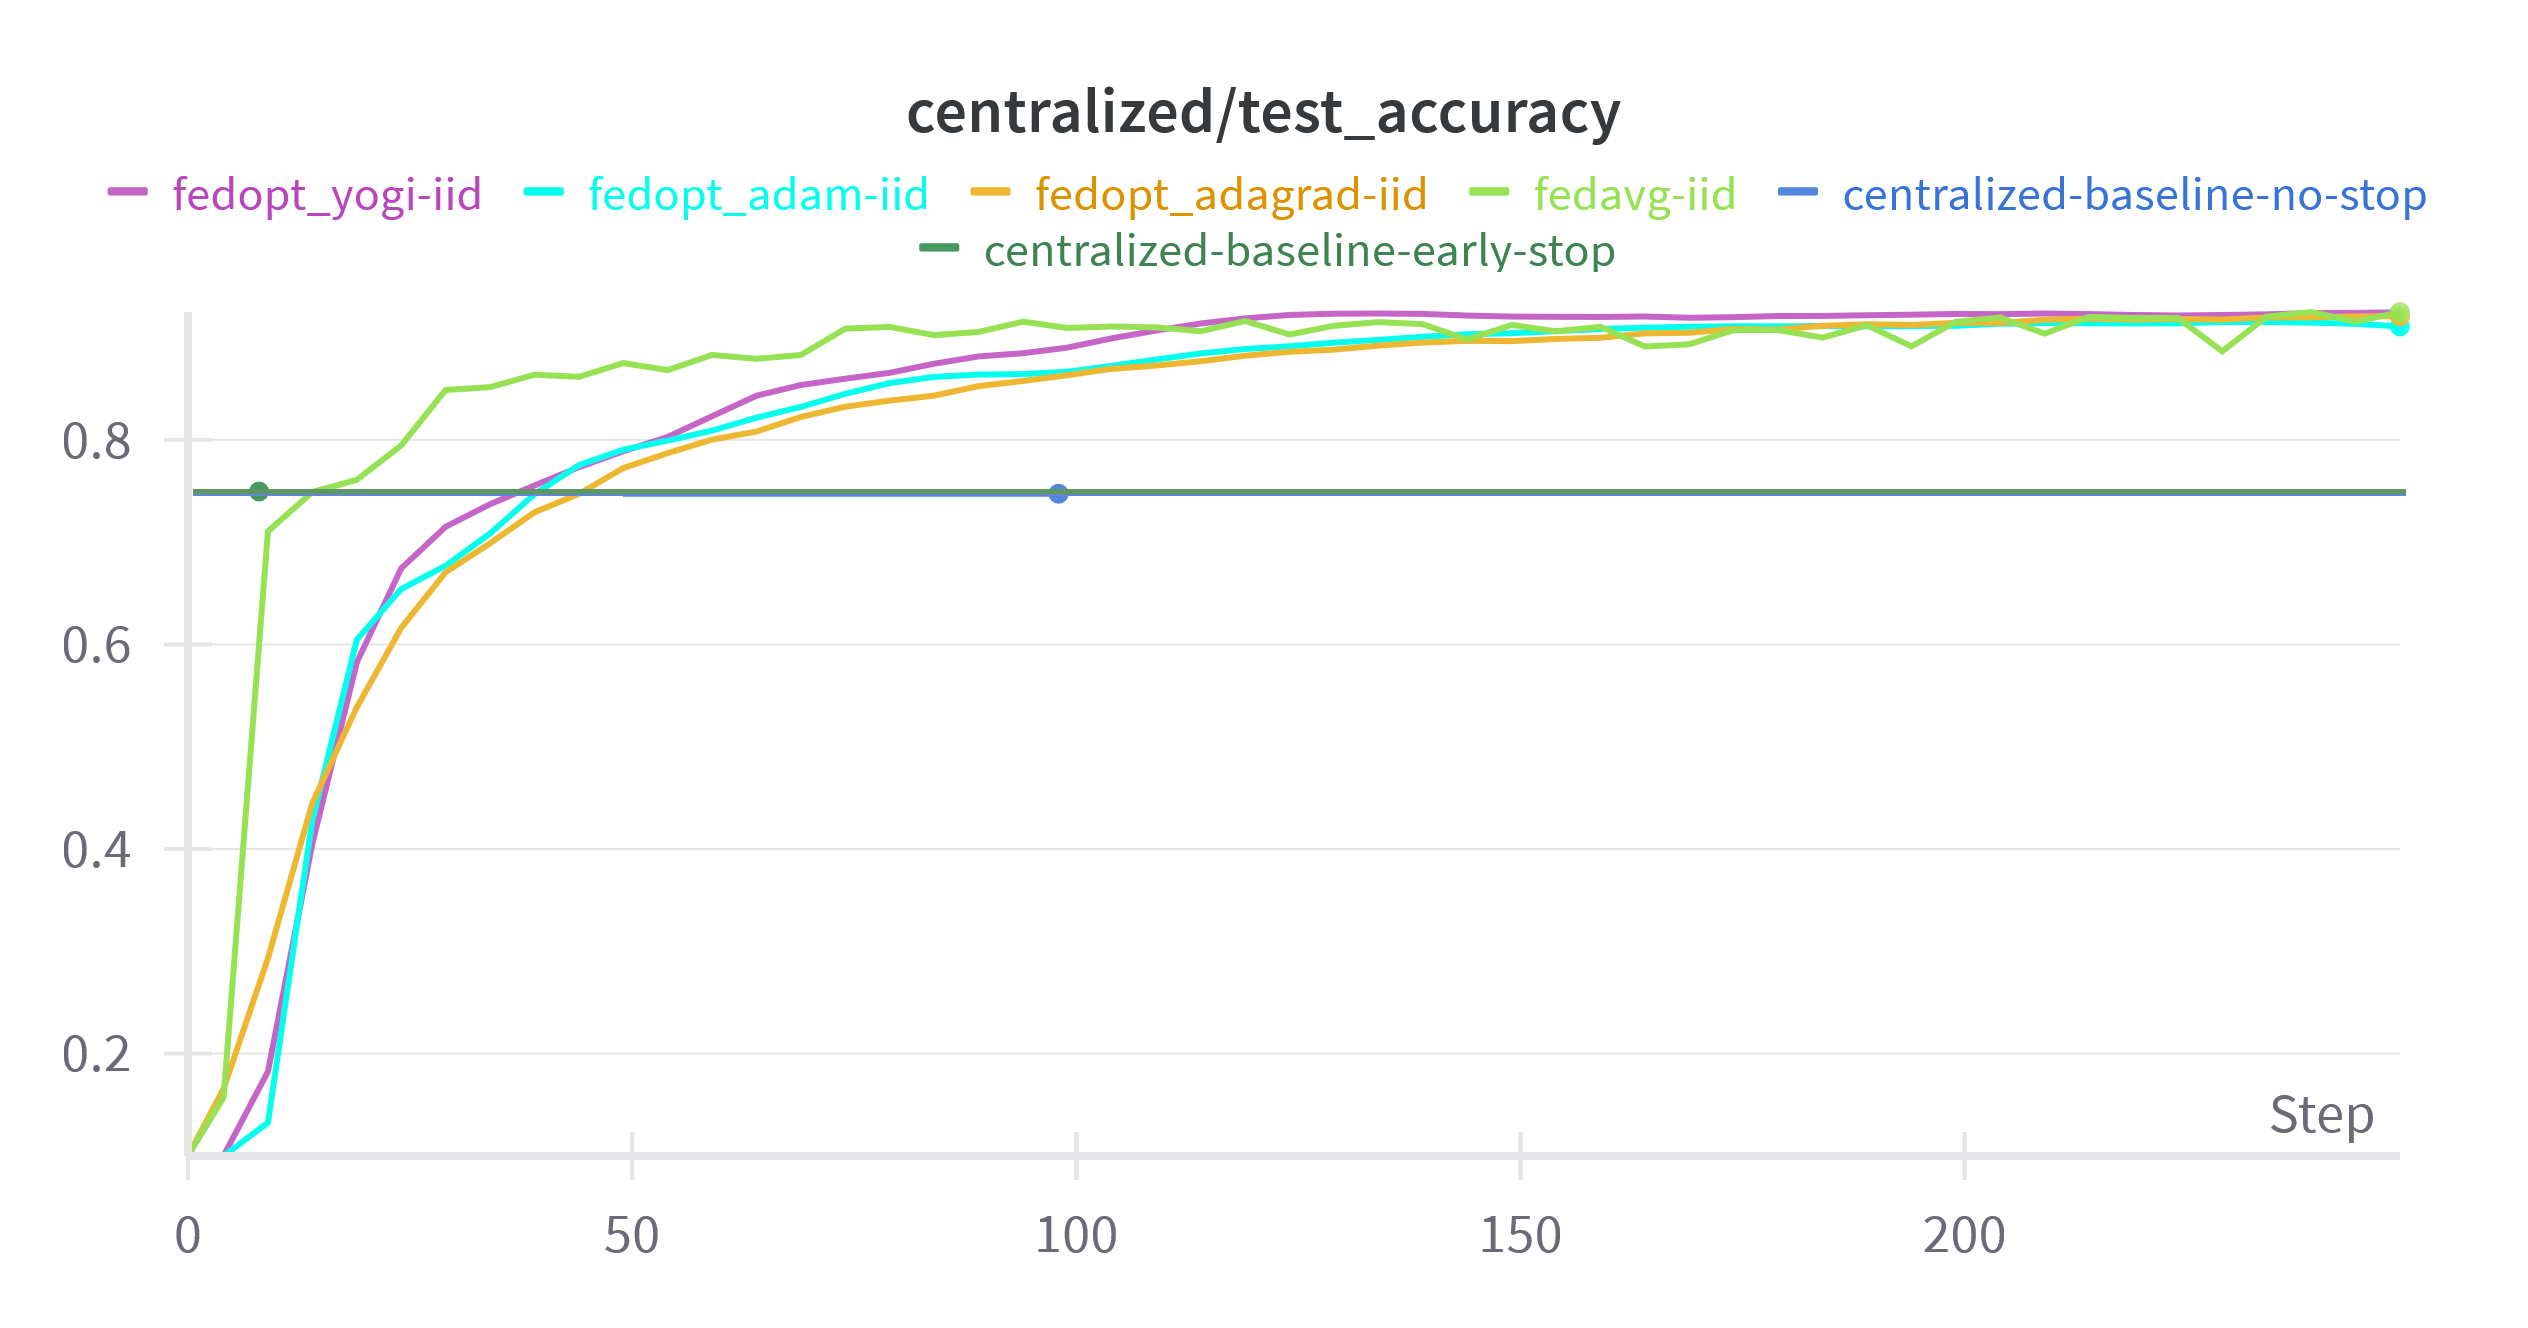
\includegraphics[width=\textwidth]{img/experiment_1/iid_server_test_acc}
            \caption{Global model test accuracy}
            \label{fig:iid_global_val_acc}
        \end{subfigure}
        \caption{Global model performance metrics evolution for IID partitioning}
        \label{fig:iid_global_metrics}
    \end{figure}

    \textbf{Performance Summary}

    Table~\ref{tab:iid_performance} summarizes the final performance metrics for all tested federated optimization strategies under IID data distribution. The results reveal that FedOpt with Adam optimizer achieves the highest final accuracy 66\%, while FedOpt with Yogi demonstrates the fastest convergence, requiring only 24 rounds to reach stable performance.

    \begin{table}[h]
        \centering
        \caption{Performance comparison of federated optimization strategies under IID partitioning}
        \label{tab:iid_performance}
        \begin{tabular}{|l|c|c|c|}
            \hline
            \textbf{Strategy} & \textbf{Final Accuracy} & \textbf{Final Loss} & \textbf{Rounds to Converge} \\
            \hline
            FedAvg            & 0.92                    & 0.64                & 47                          \\
            FedOpt (AdaGrad)  & 0.92                    & 0.30                & 40                          \\
            FedOpt (Adam)     & 0.92                    & 0.66                & 40                          \\
            FedOpt (Yogi)     & 0.91                    & 0.64                & 24                          \\
            \hline
        \end{tabular}
    \end{table}

    The performance analysis indicates that while FedAvg provides a solid baseline with 64\% accuracy, the choice of optimizer in FedOpt significantly impacts both final performance and convergence speed.

    \subsubsection{Square Partitioning Scenario}
    \label{subsubsec:square-scenario}

    In this scenario, each client has an imbalanced distribution of samples, with the amount of samples varying with the square of the client index. This creates a highly heterogeneous data distribution where some clients have significantly more training data than others, as illustrated in Figure~\ref{fig:square_partitioning}.

    The square partitioning scenario presents a more challenging federated learning environment compared to IID conditions, as the significant data imbalance between clients can lead to training instabilities and convergence issues. Figure~\ref{fig:square_client_metrics} shows the client-averaged validation metrics, while Figure~\ref{fig:square_global_metrics} presents the global model performance on the test set.

    \begin{figure}[h]
        \centering
        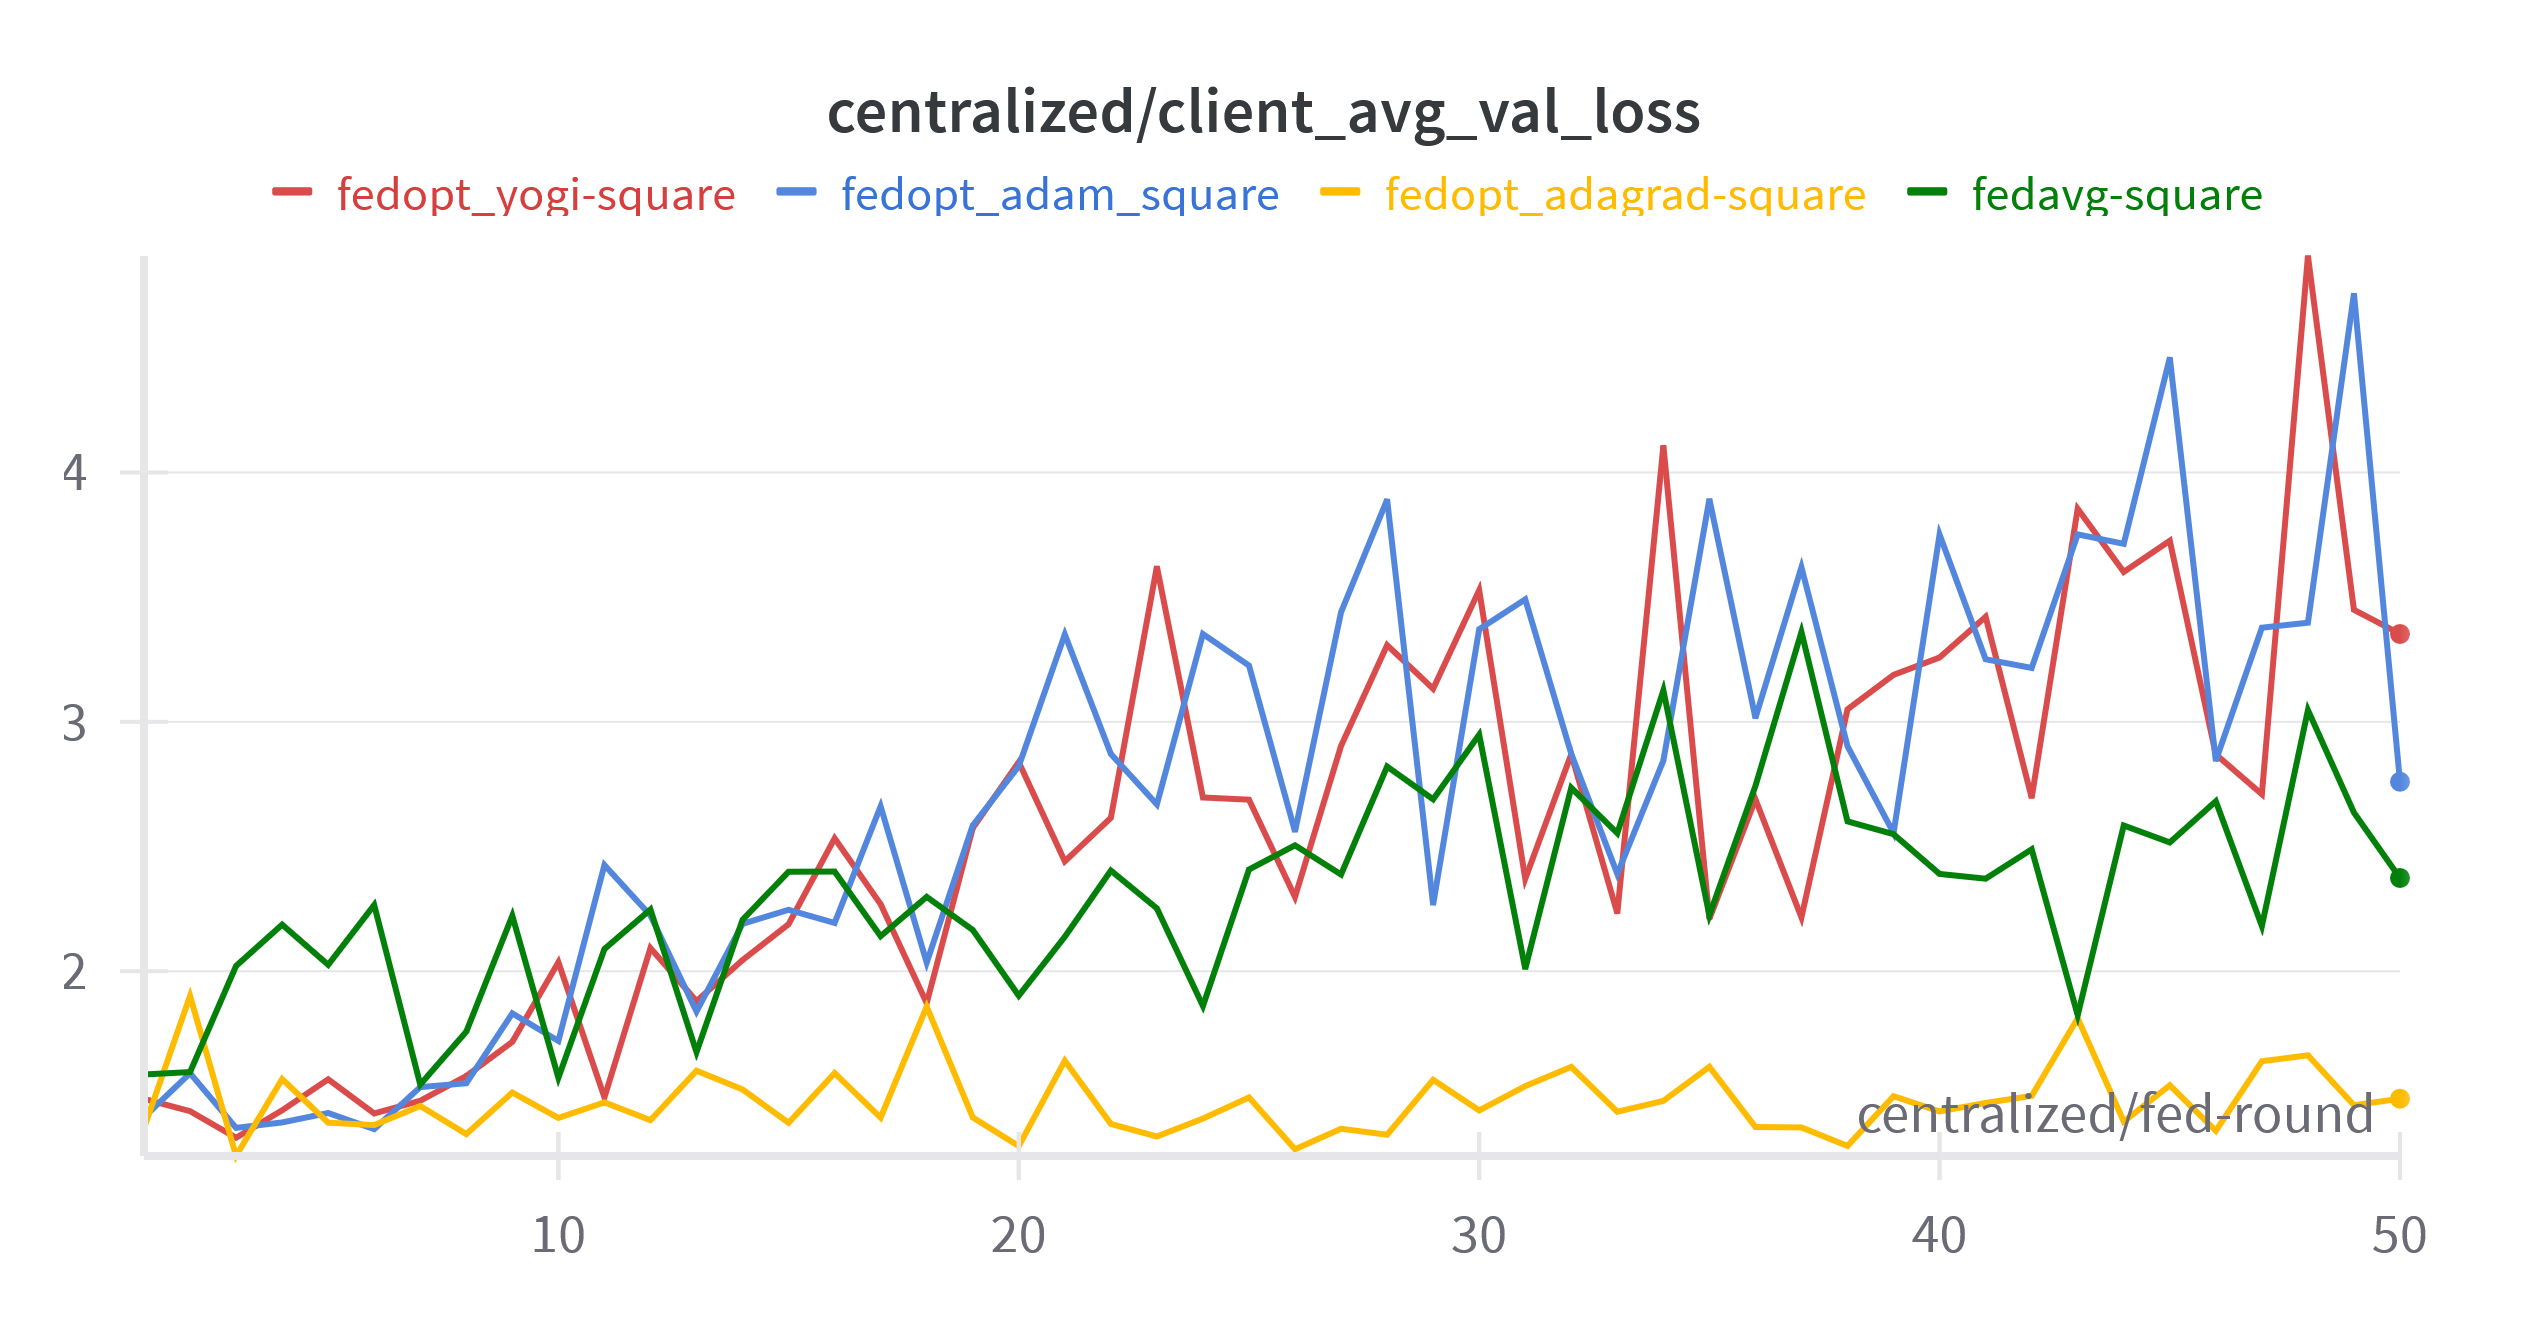
\includegraphics[width=0.48\textwidth]{img/experiment_1/square_client_avg_val_loss}
        \hfill
        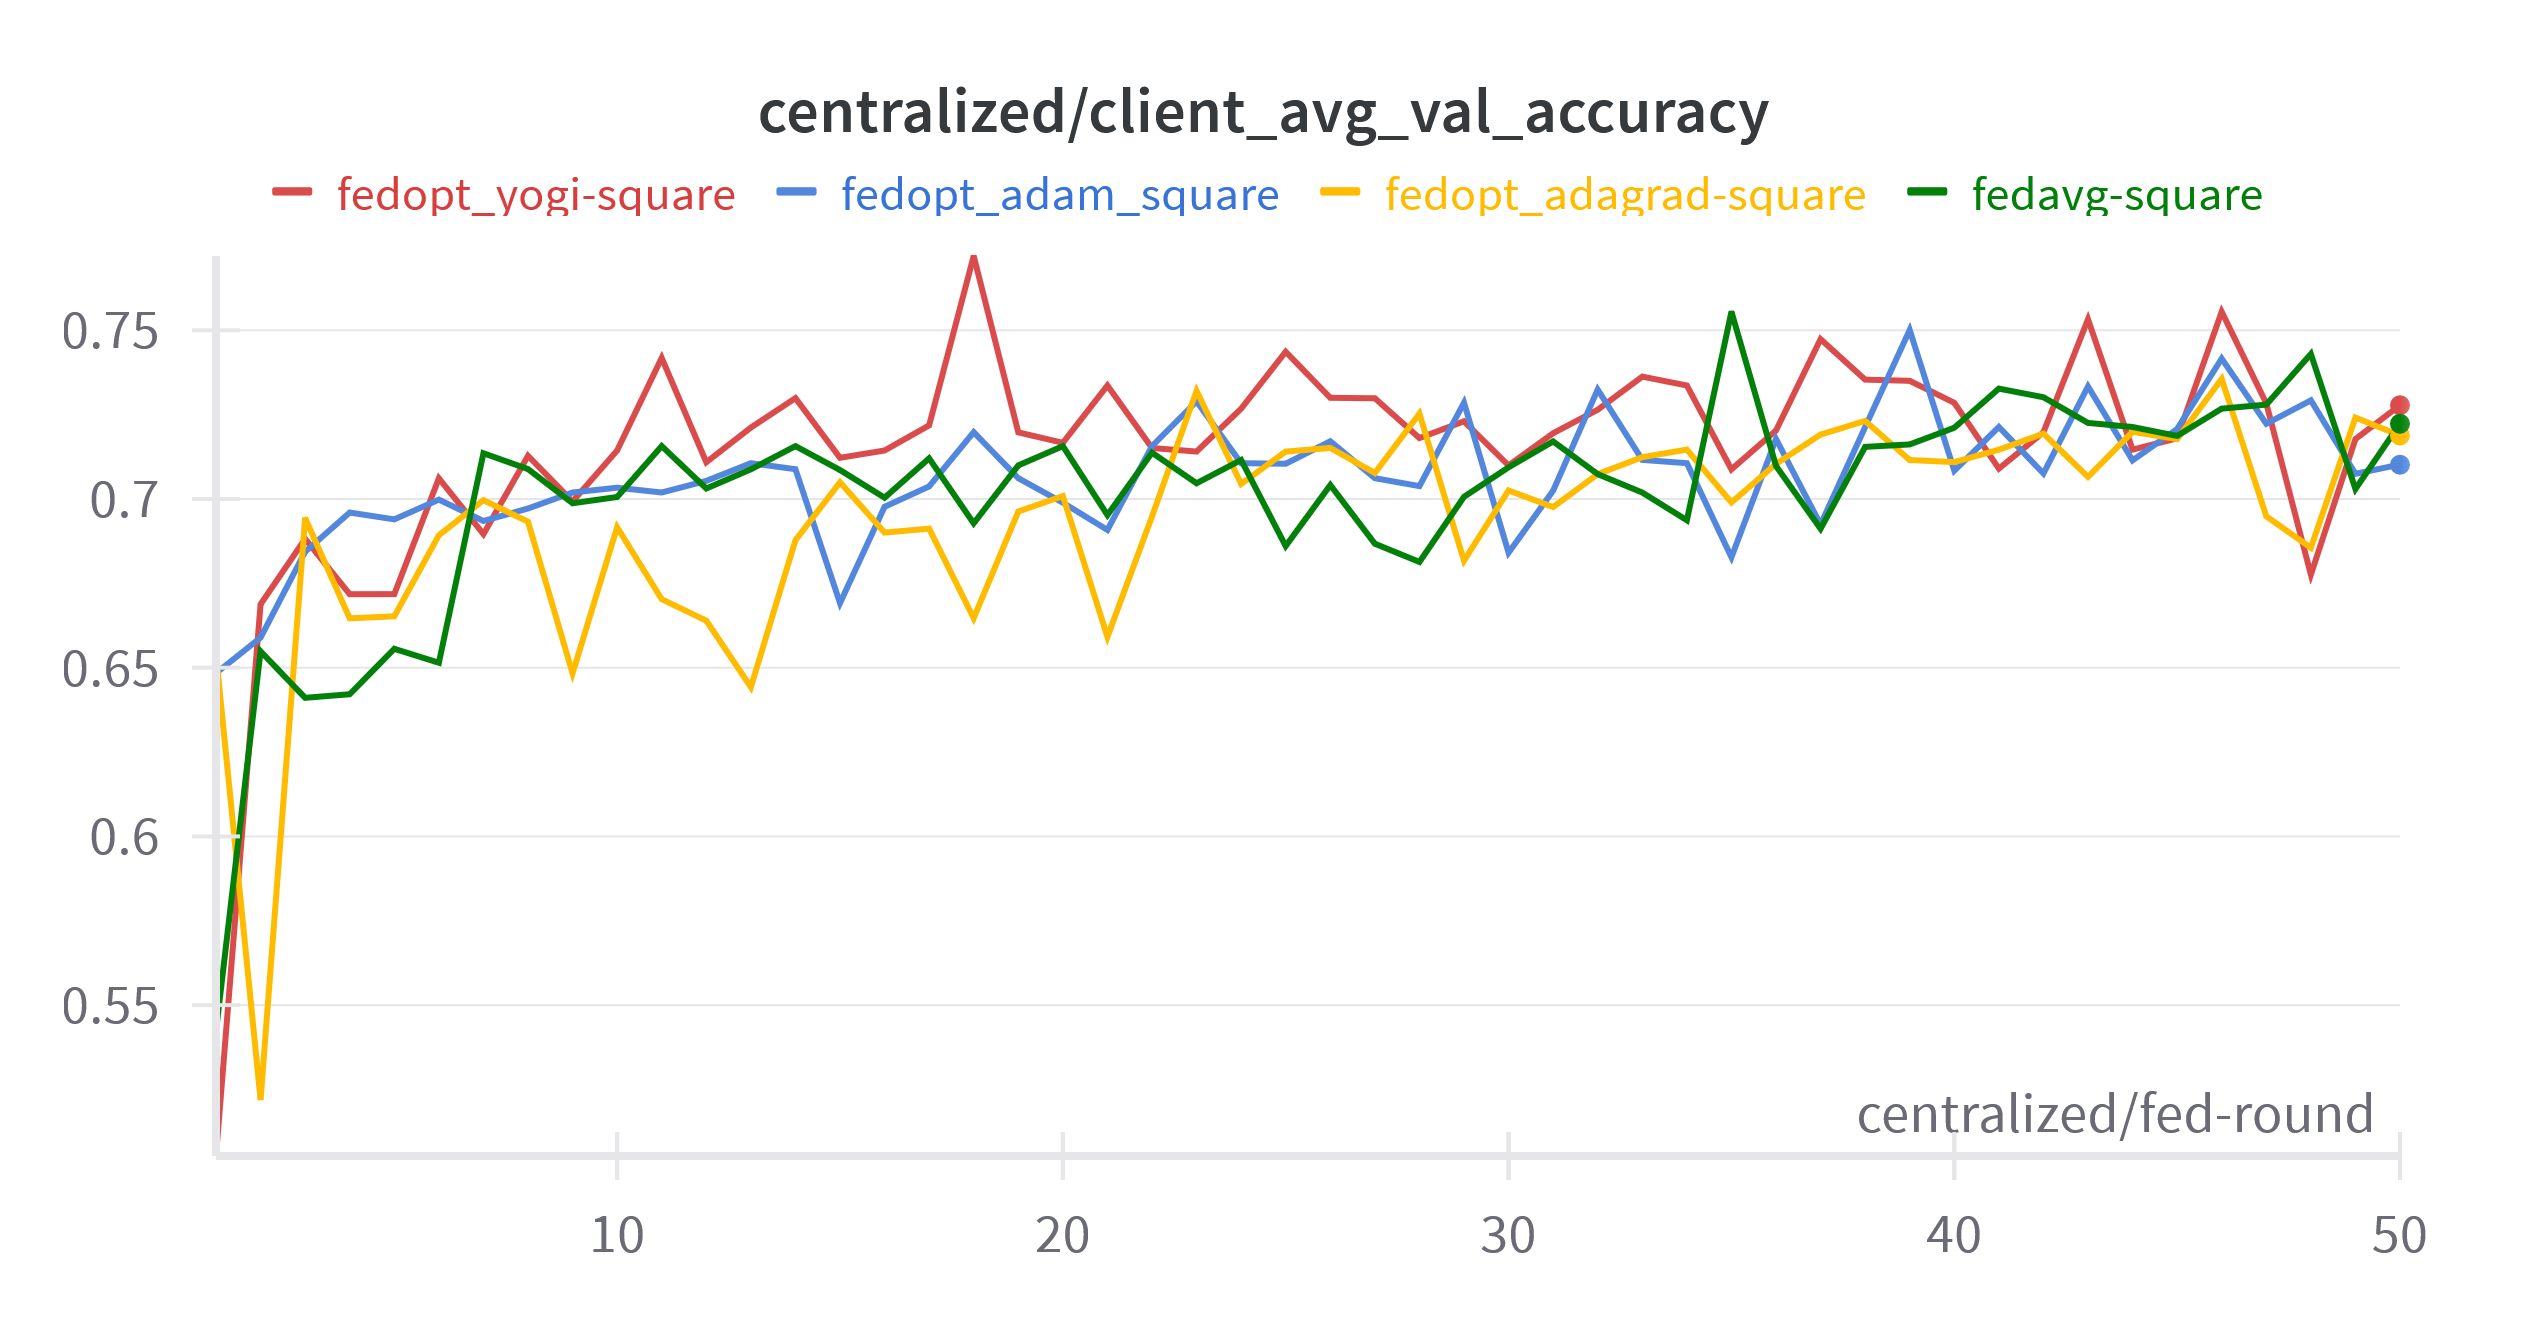
\includegraphics[width=0.48\textwidth]{img/experiment_1/square_client_avg_val_acc}
        \caption{Client-side performance metrics: validation loss (left) and accuracy (right) evolution during training for square partitioning}
        \label{fig:square_client_metrics}
    \end{figure}

    \begin{figure}[h]
        \centering
        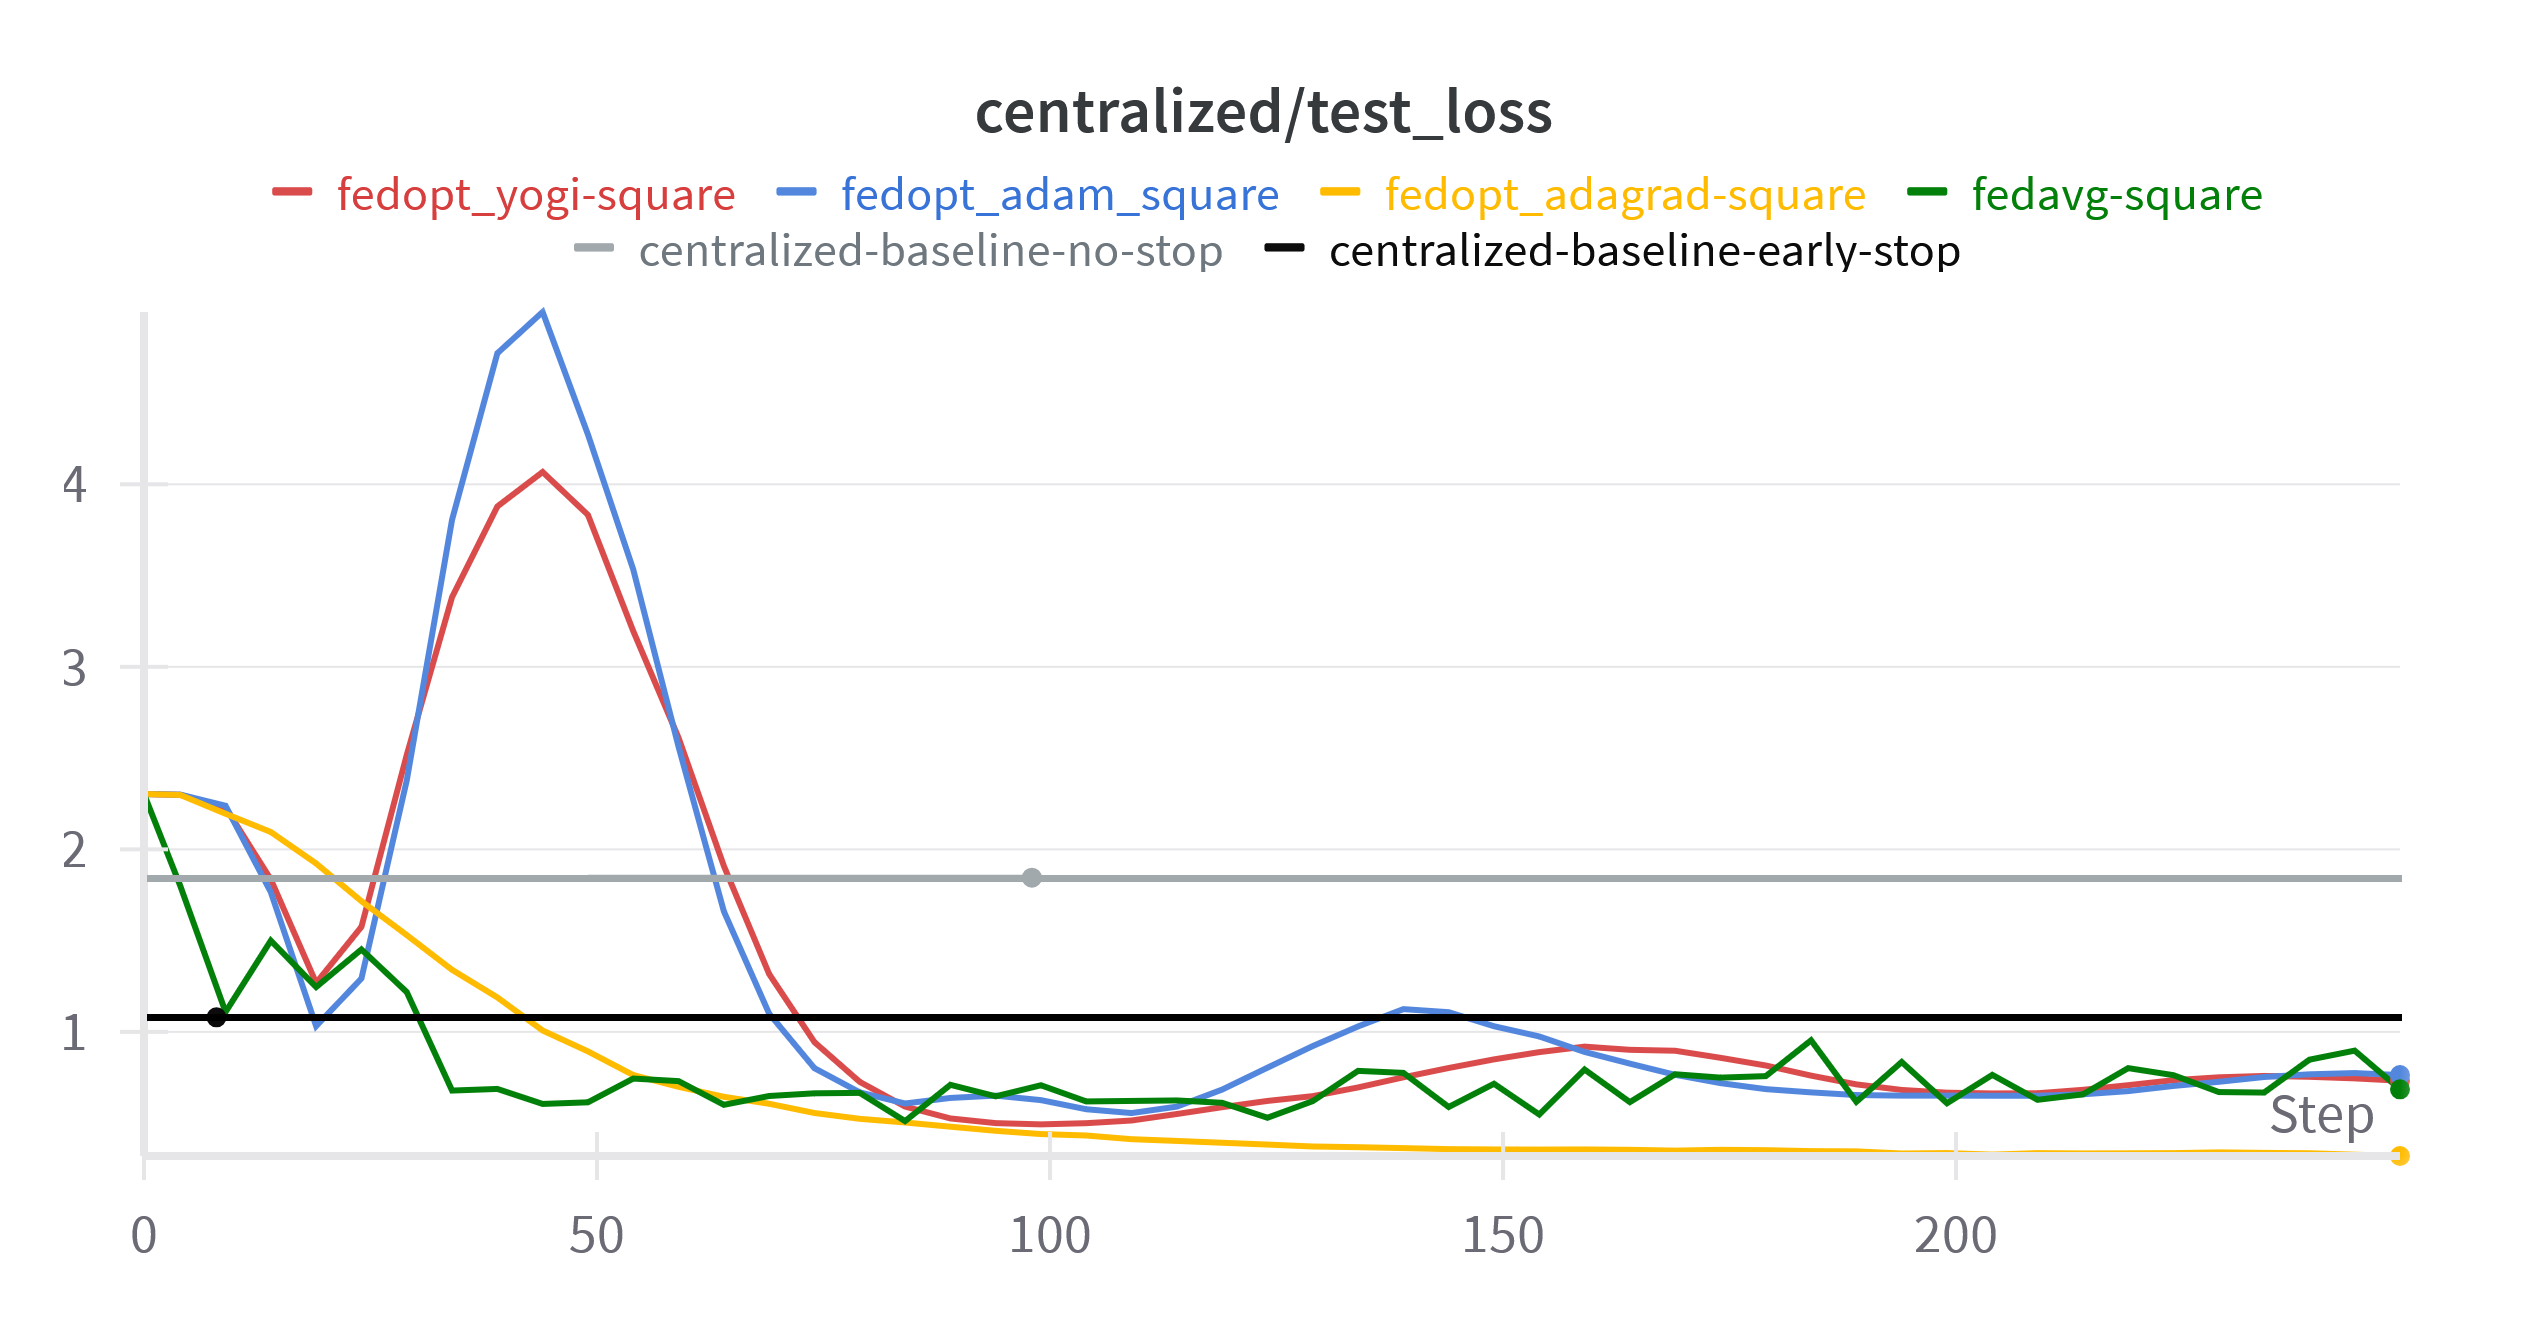
\includegraphics[width=0.48\textwidth]{img/experiment_1/square_server_test_loss}
        \hfill
        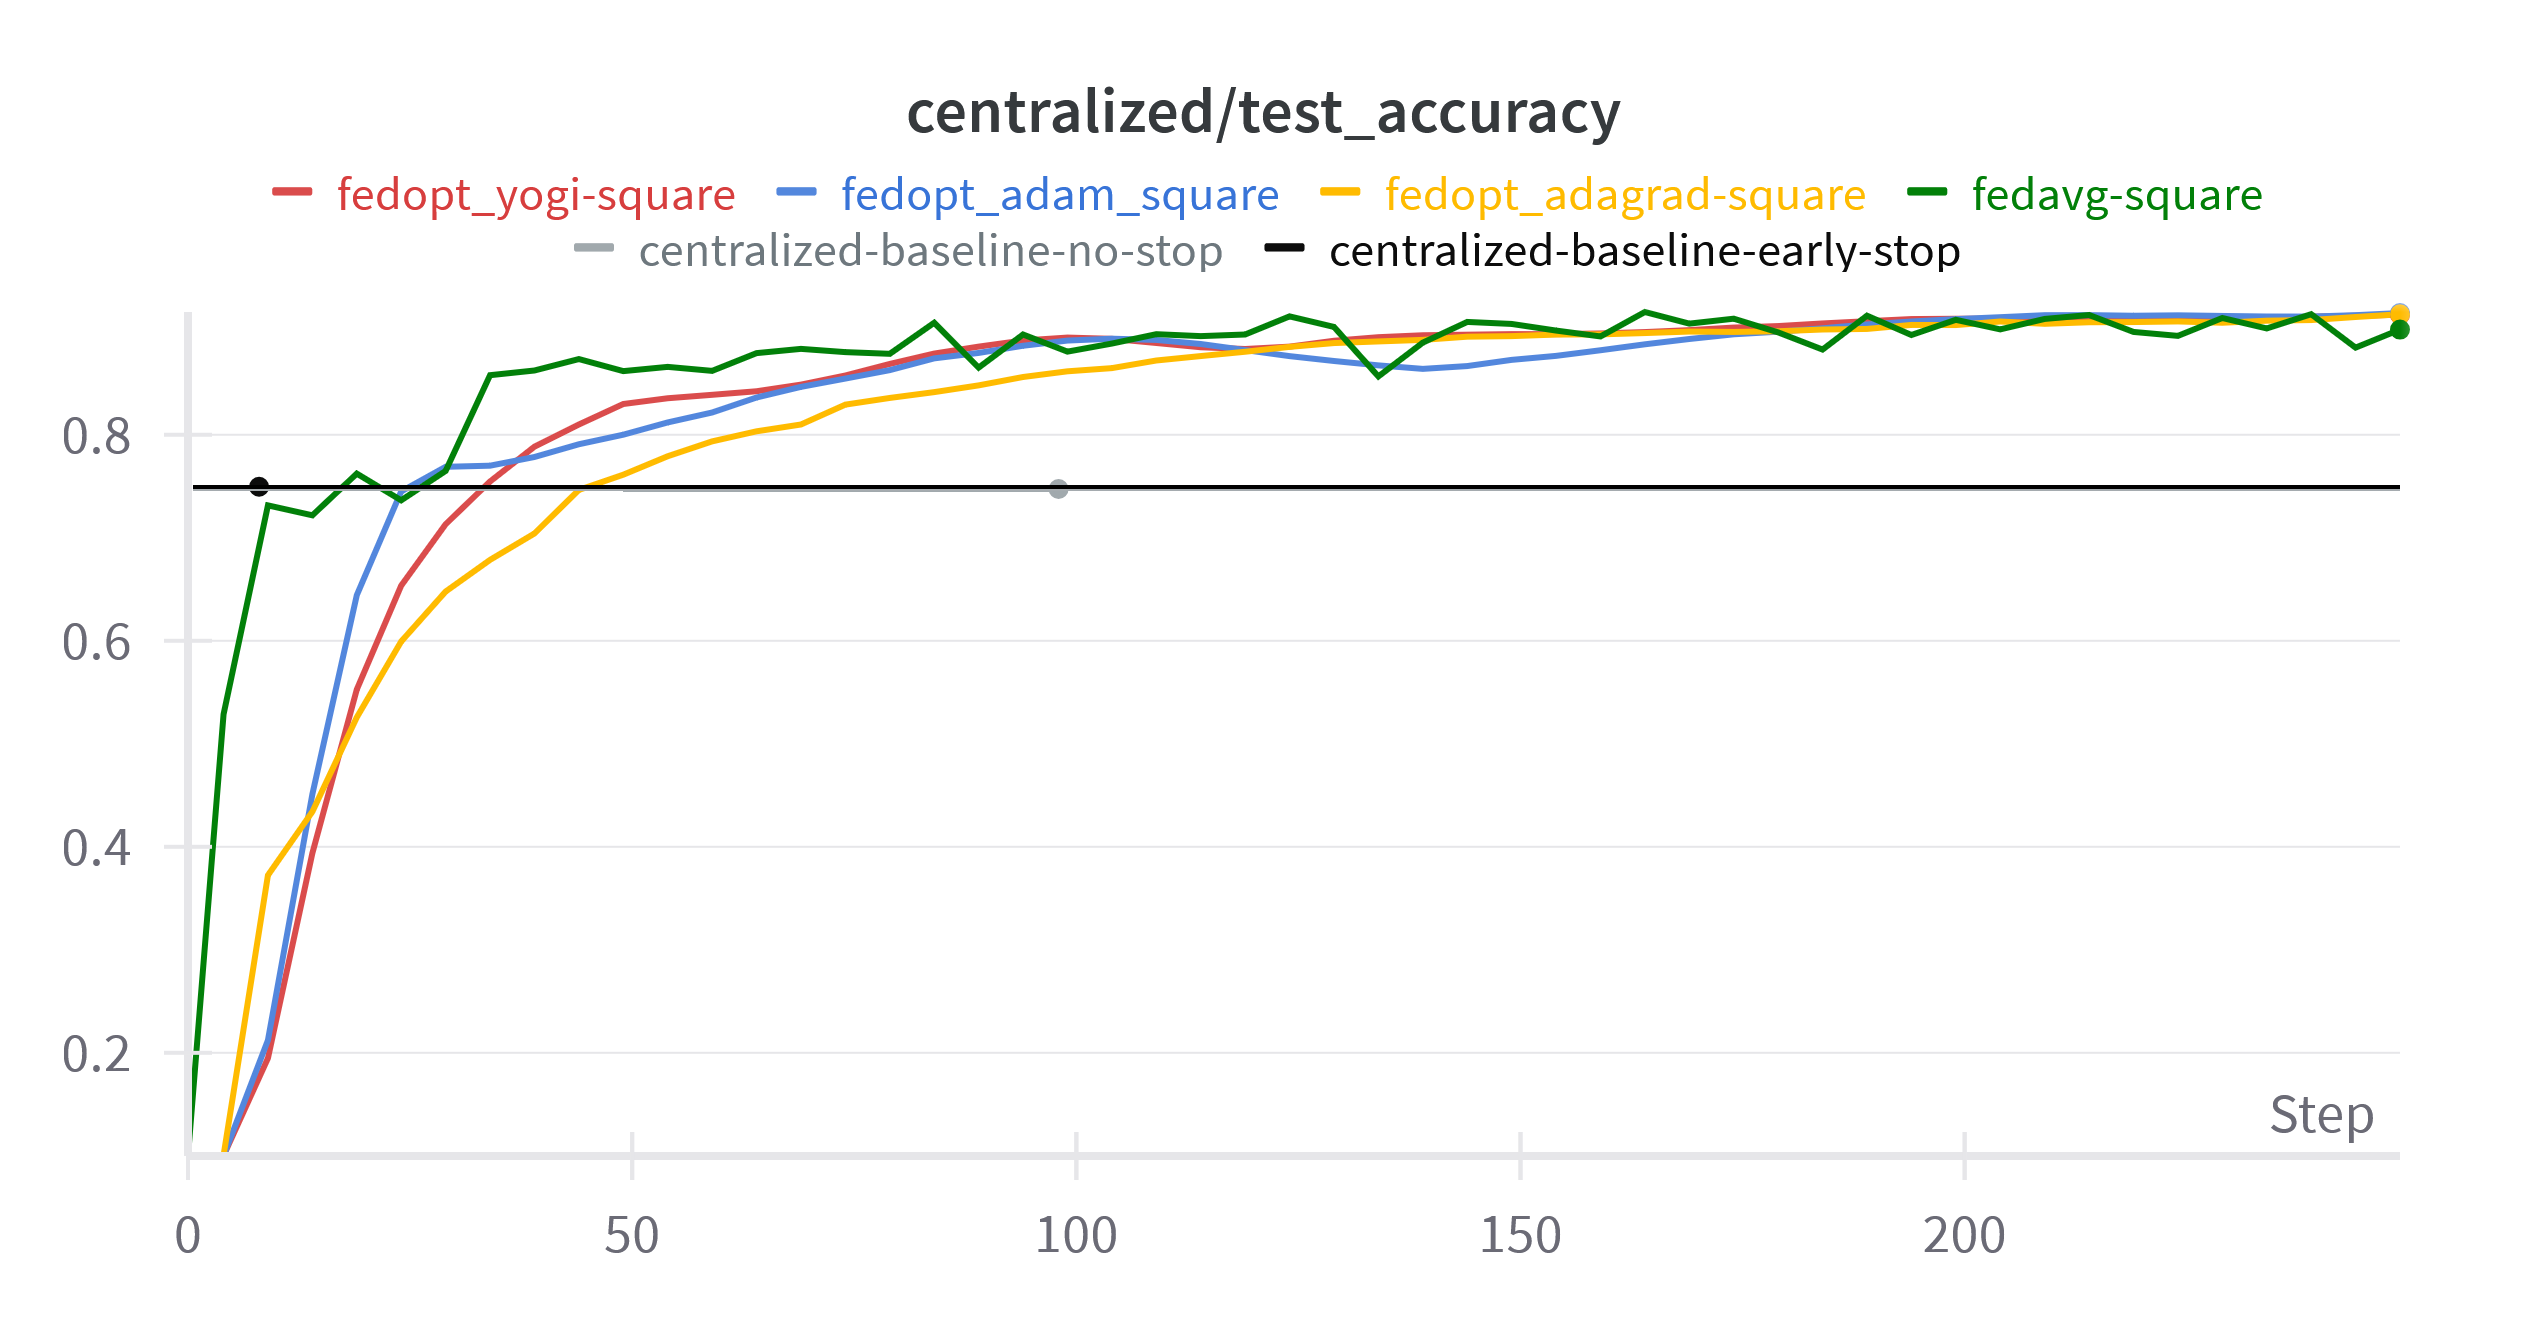
\includegraphics[width=0.48\textwidth]{img/experiment_1/square_server_test_acc}
        \caption{Global model performance metrics: test loss (left) and accuracy (right) evolution for square partitioning}
        \label{fig:square_global_metrics}
    \end{figure}

    \noindent
    \textbf{Performance Summary}


    Table~\ref{tab:square_performance} summarizes the final performance metrics for all tested federated optimization strategies under square partitioning. The results demonstrate that data imbalance significantly impacts algorithm performance, with \texttt{FedOpt} using \texttt{Adam} optimizer achieving the highest final accuracy (0.918), representing a notable improvement over the baseline \texttt{FedAvg} approach.

    \begin{table}[h]
        \centering
        \caption{Performance comparison of federated optimization strategies under square partitioning}
        \label{tab:square_performance}
        \begin{tabular}{|l|c|c|c|}
            \hline
            \textbf{Strategy} & \textbf{Final Accuracy} & \textbf{Final Loss} & \textbf{Rounds to Converge} \\
            \hline
            FedAvg            & 0.902                   & 0.68                & N/A                         \\
            FedOpt (AdaGrad)  & 0.916                   & 0.32                & 38                          \\
            FedOpt (Adam)     & 0.918                   & 0.76                & 39                          \\
            FedOpt (Yogi)     & 0.916                   & 0.73                & 38                          \\
            \hline
        \end{tabular}
    \end{table}

    The performance analysis reveals interesting patterns under data imbalance conditions. While \texttt{FedAvg} shows strong baseline performance with 90.2\% accuracy, it fails to converge within the observation period. \texttt{FedOpt} with \texttt{Adam} demonstrates the most robust performance, achieving 91.8\% accuracy---the highest among all tested configurations. Both \texttt{Adam} and \texttt{Yogi} optimizers show enhanced performance compared to \texttt{FedAvg}, with \texttt{Adam} achieving the best accuracy and \texttt{Yogi} matching \texttt{AdaGrad} at 91.6\%. Notably, \texttt{AdaGrad} achieves the lowest final loss (0.32) among the \texttt{FedOpt} variants, suggesting good convergence properties, while \texttt{Adam} has the highest loss (0.76) despite achieving the best accuracy. All \texttt{FedOpt} variants converge within 38--39 rounds, demonstrating efficient optimization in heterogeneous federated environments.

    \subsubsection{Dirichlet Partitioning Scenario}
    \label{subsubsec:dirichlet-scenario}

    In this scenario, each client has an imbalanced distribution of both samples and classes, with the class distribution following a Dirichlet distribution. This creates the most challenging federated learning environment, where clients not only have varying amounts of data but also different class compositions, leading to significant statistical heterogeneity as shown in Figure~\ref{fig:dirichlet_partitioning}.


    The Dirichlet partitioning represents the one of the more realistic federated learning scenario, where both data quantity and class distributions vary significantly across clients. This statistical heterogeneity poses substantial challenges for model convergence and generalization. Figure~\ref{fig:dirichlet_client_metrics} shows the client-averaged validation metrics, while Figure~\ref{fig:dirichlet_global_metrics} presents the global model performance on the test set.

    \begin{figure}[h]
        \centering
        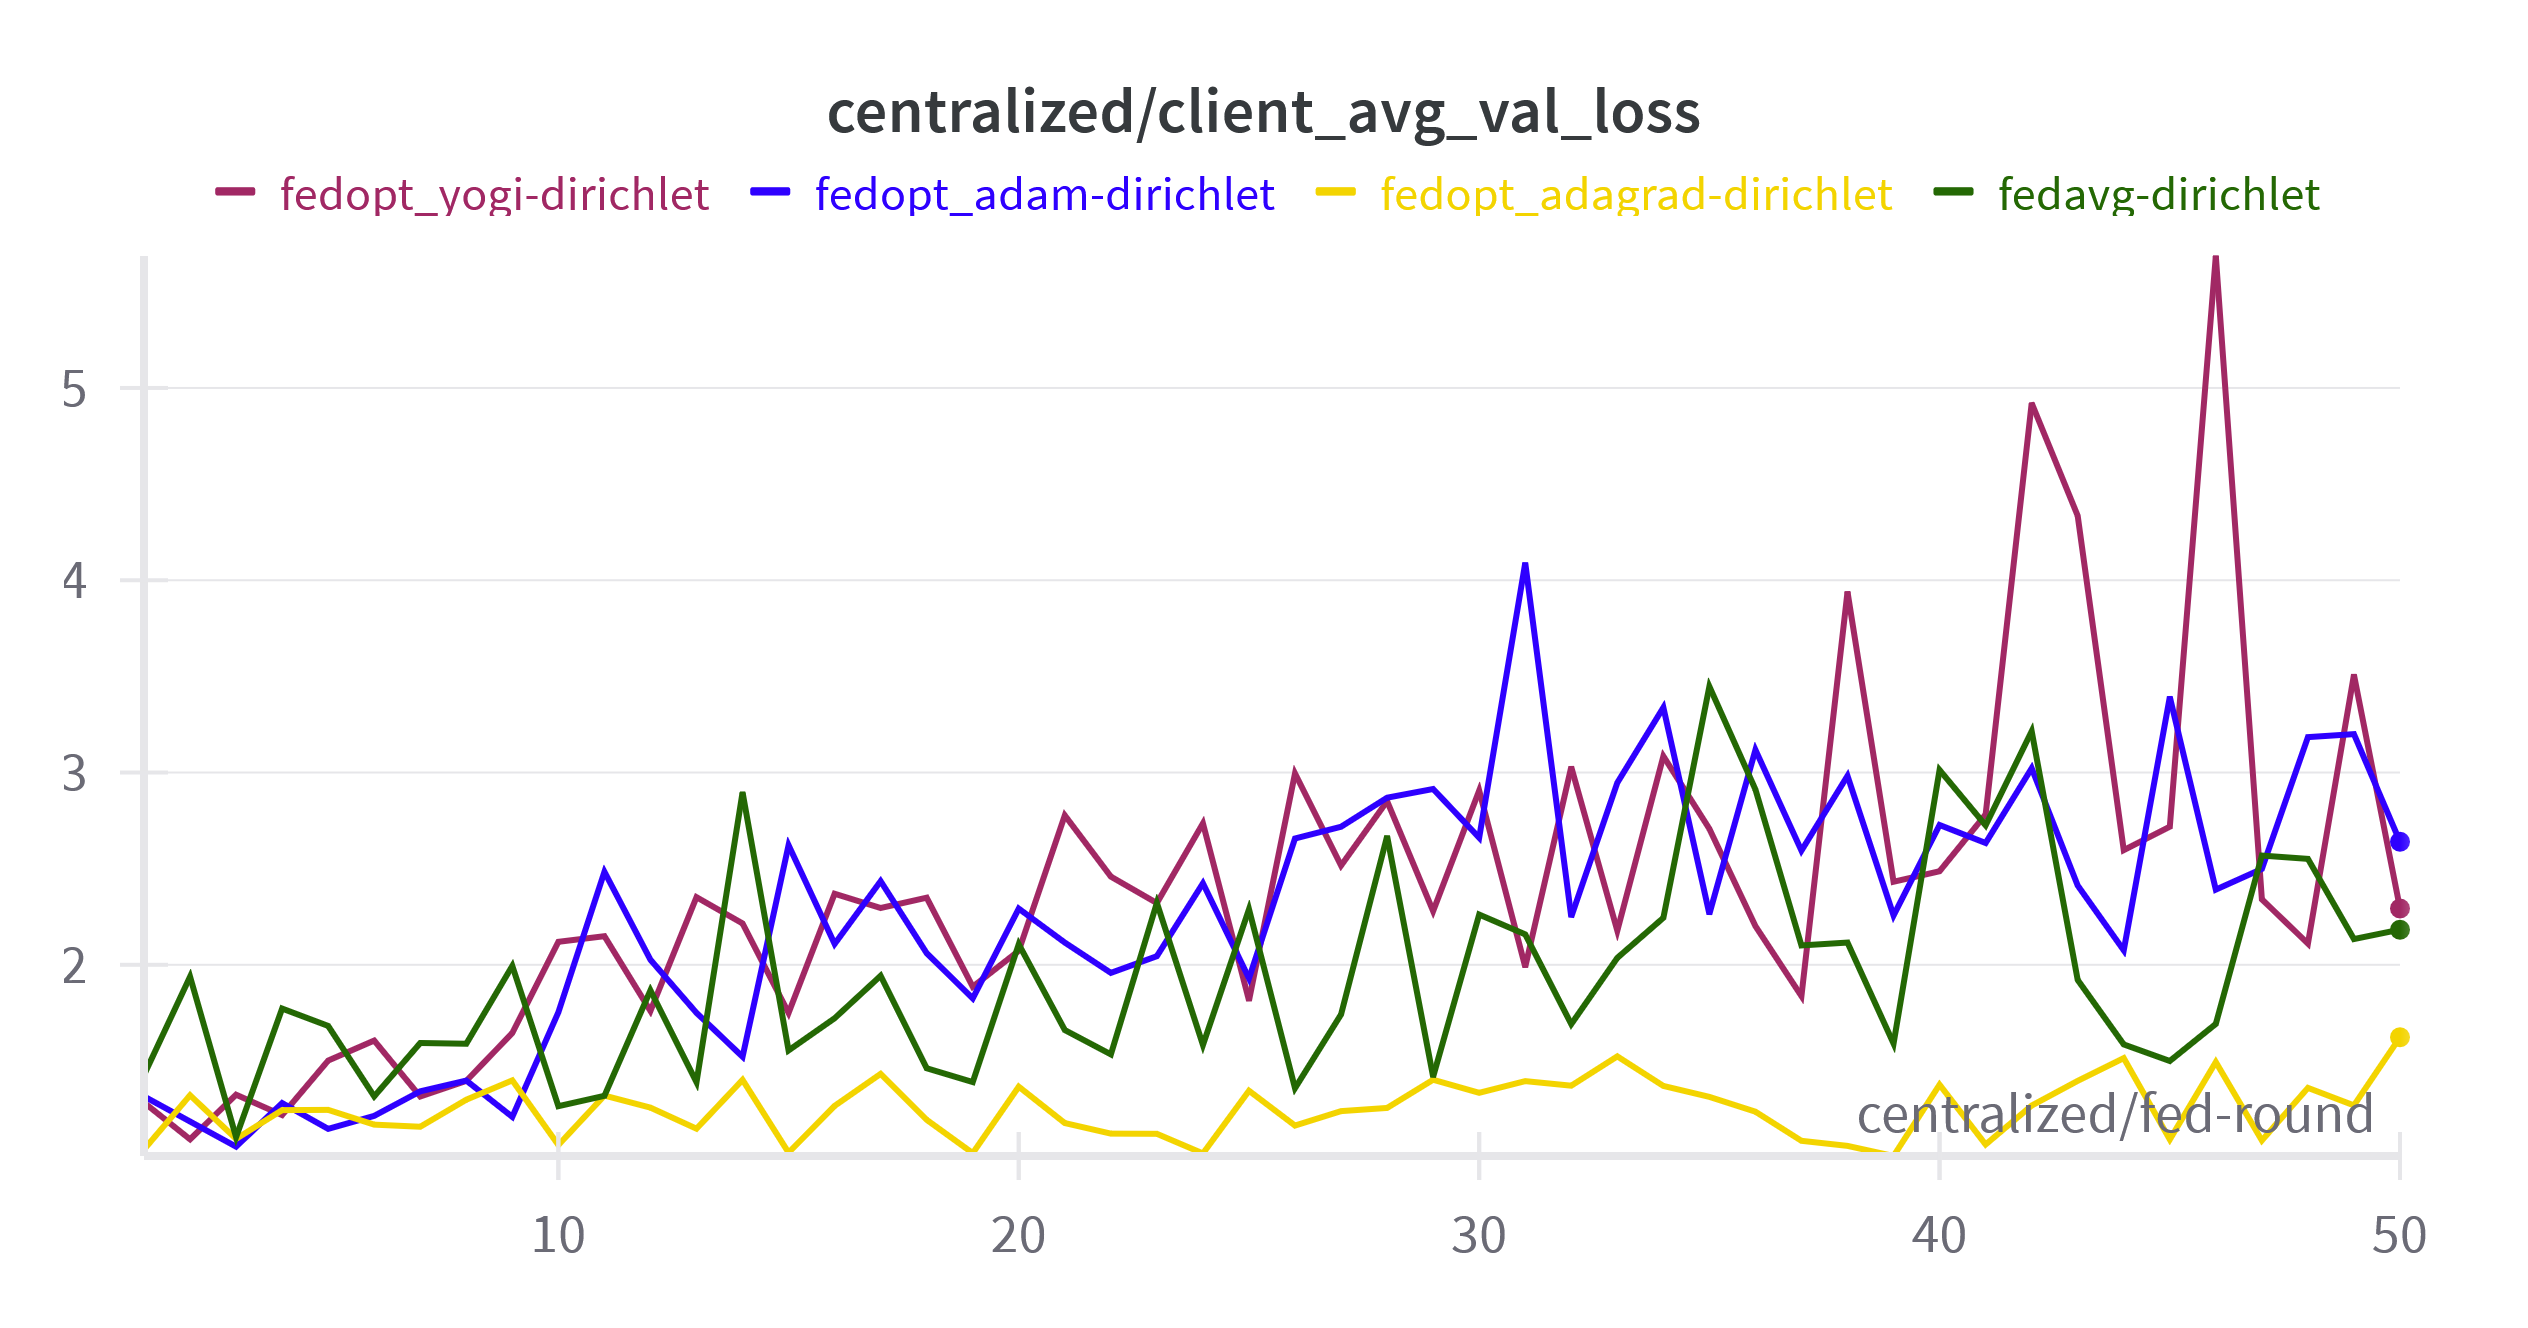
\includegraphics[width=0.48\textwidth]{img/experiment_1/dirichlet_client_avg_val_loss}
        \hfill
        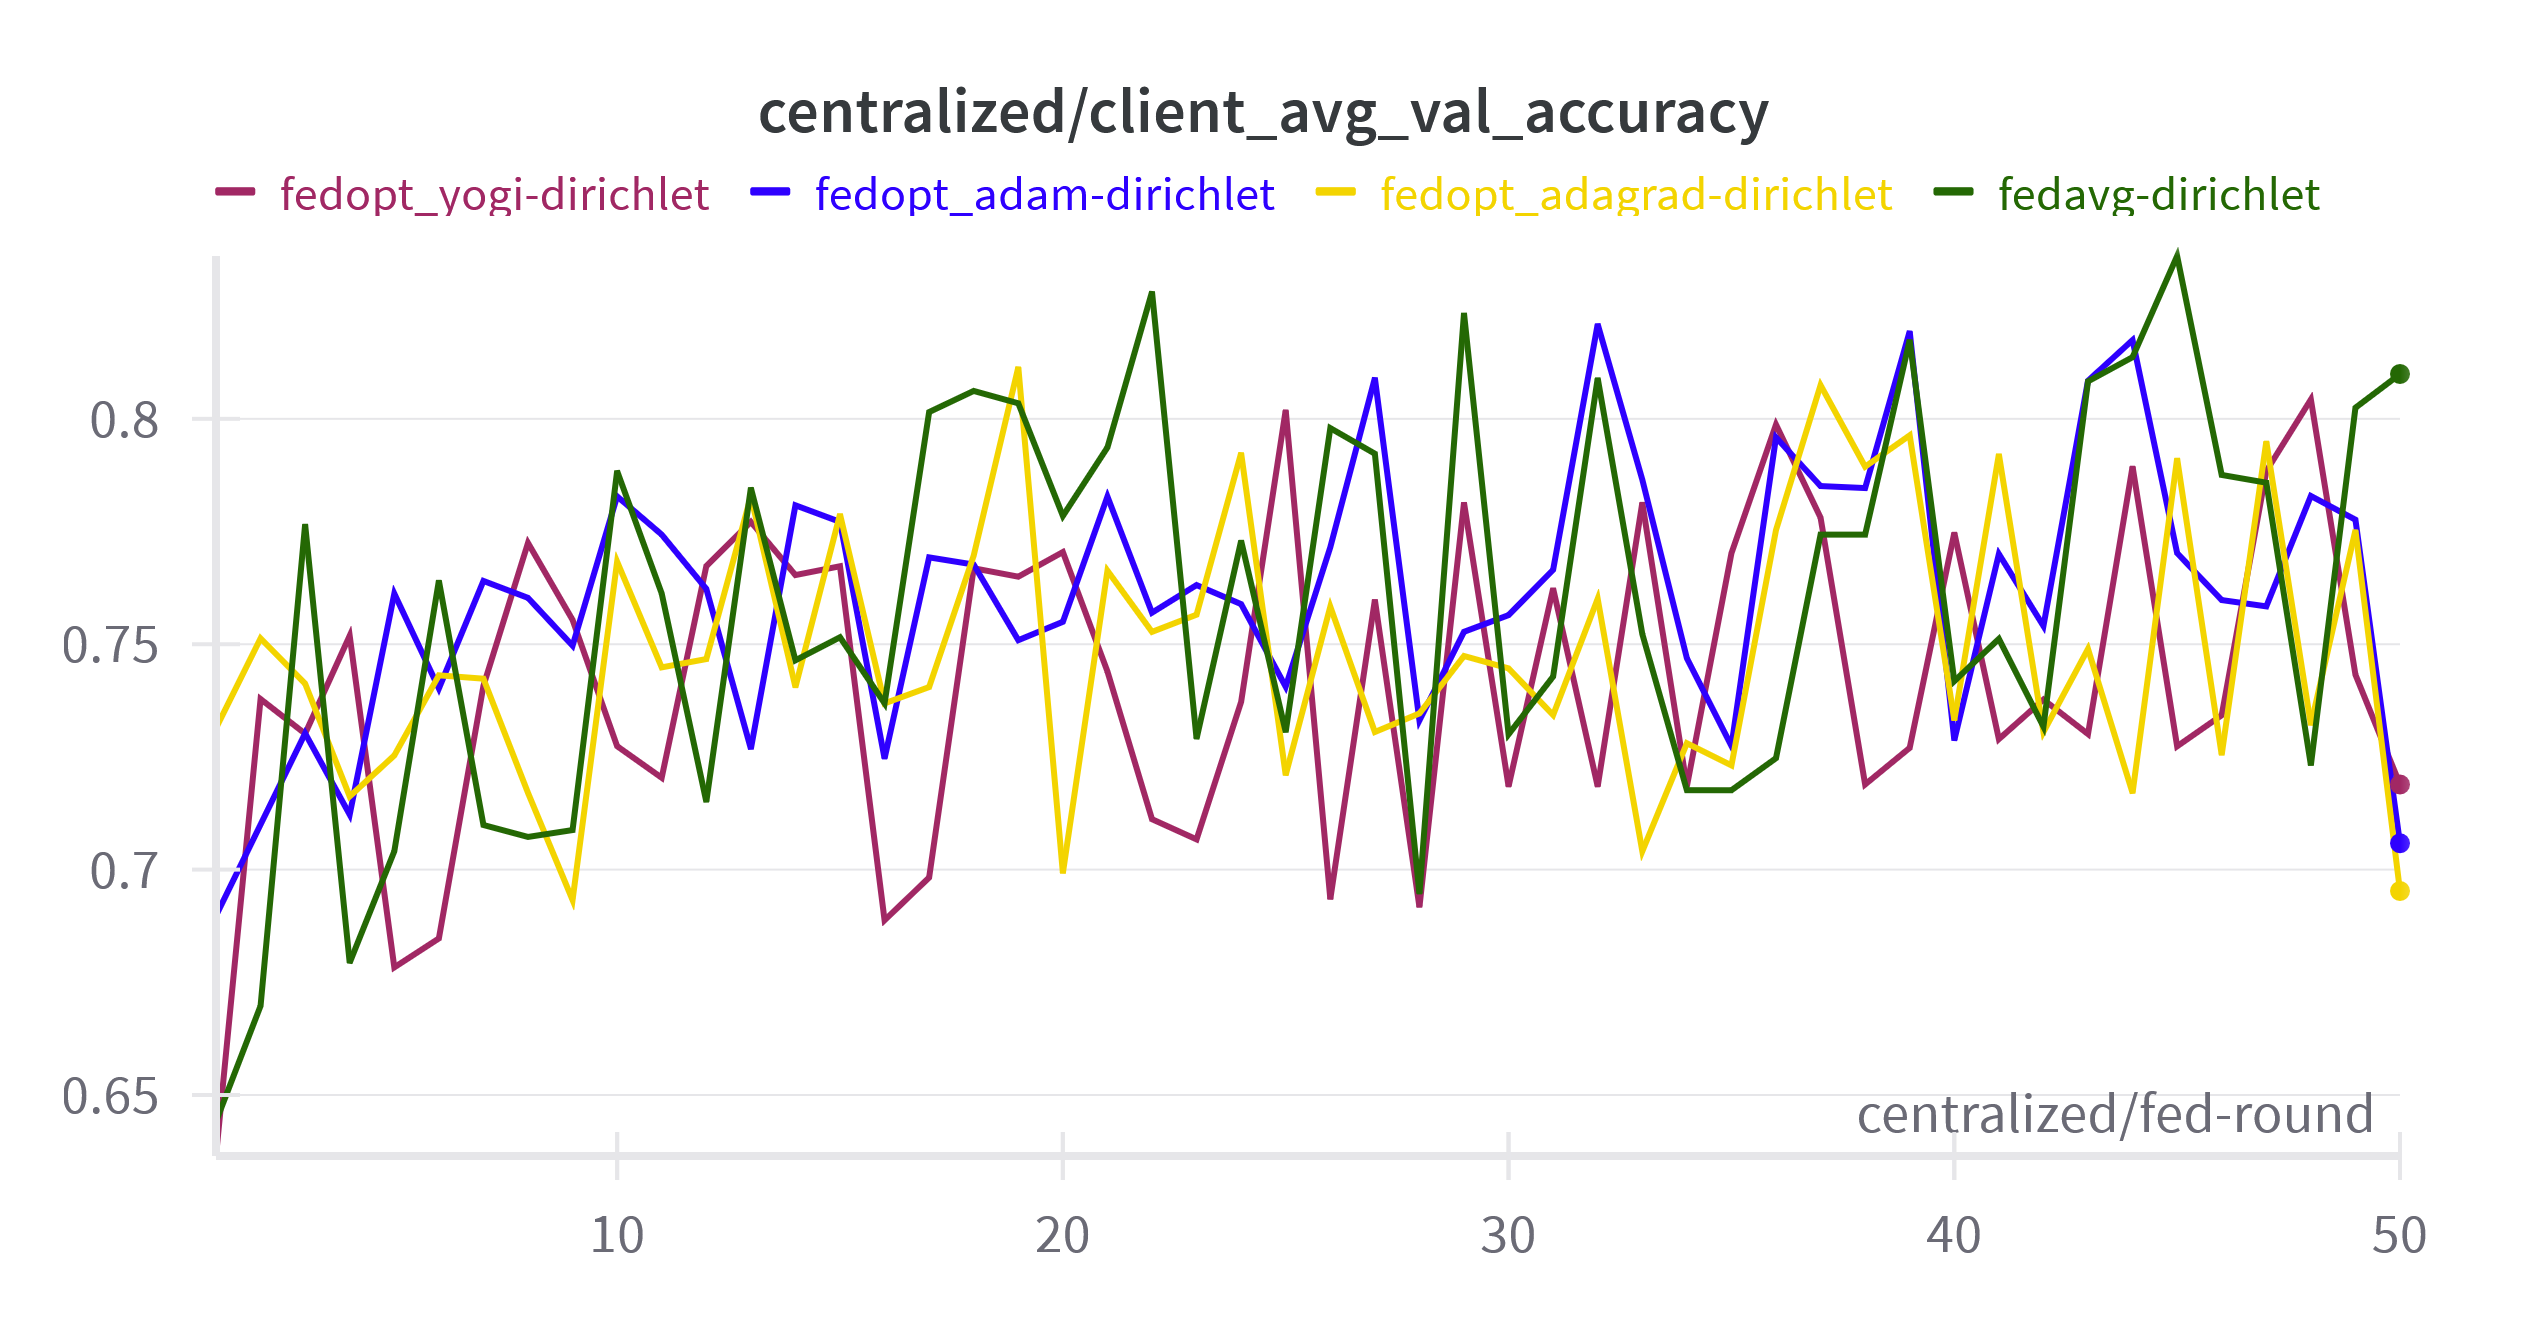
\includegraphics[width=0.48\textwidth]{img/experiment_1/dirichlet_client_avg_val_acc}
        \caption{Client-side performance metrics: validation loss (left) and accuracy (right) evolution during training for Dirichlet partitioning}
        \label{fig:dirichlet_client_metrics}
    \end{figure}

    \begin{figure}[h]
        \centering
        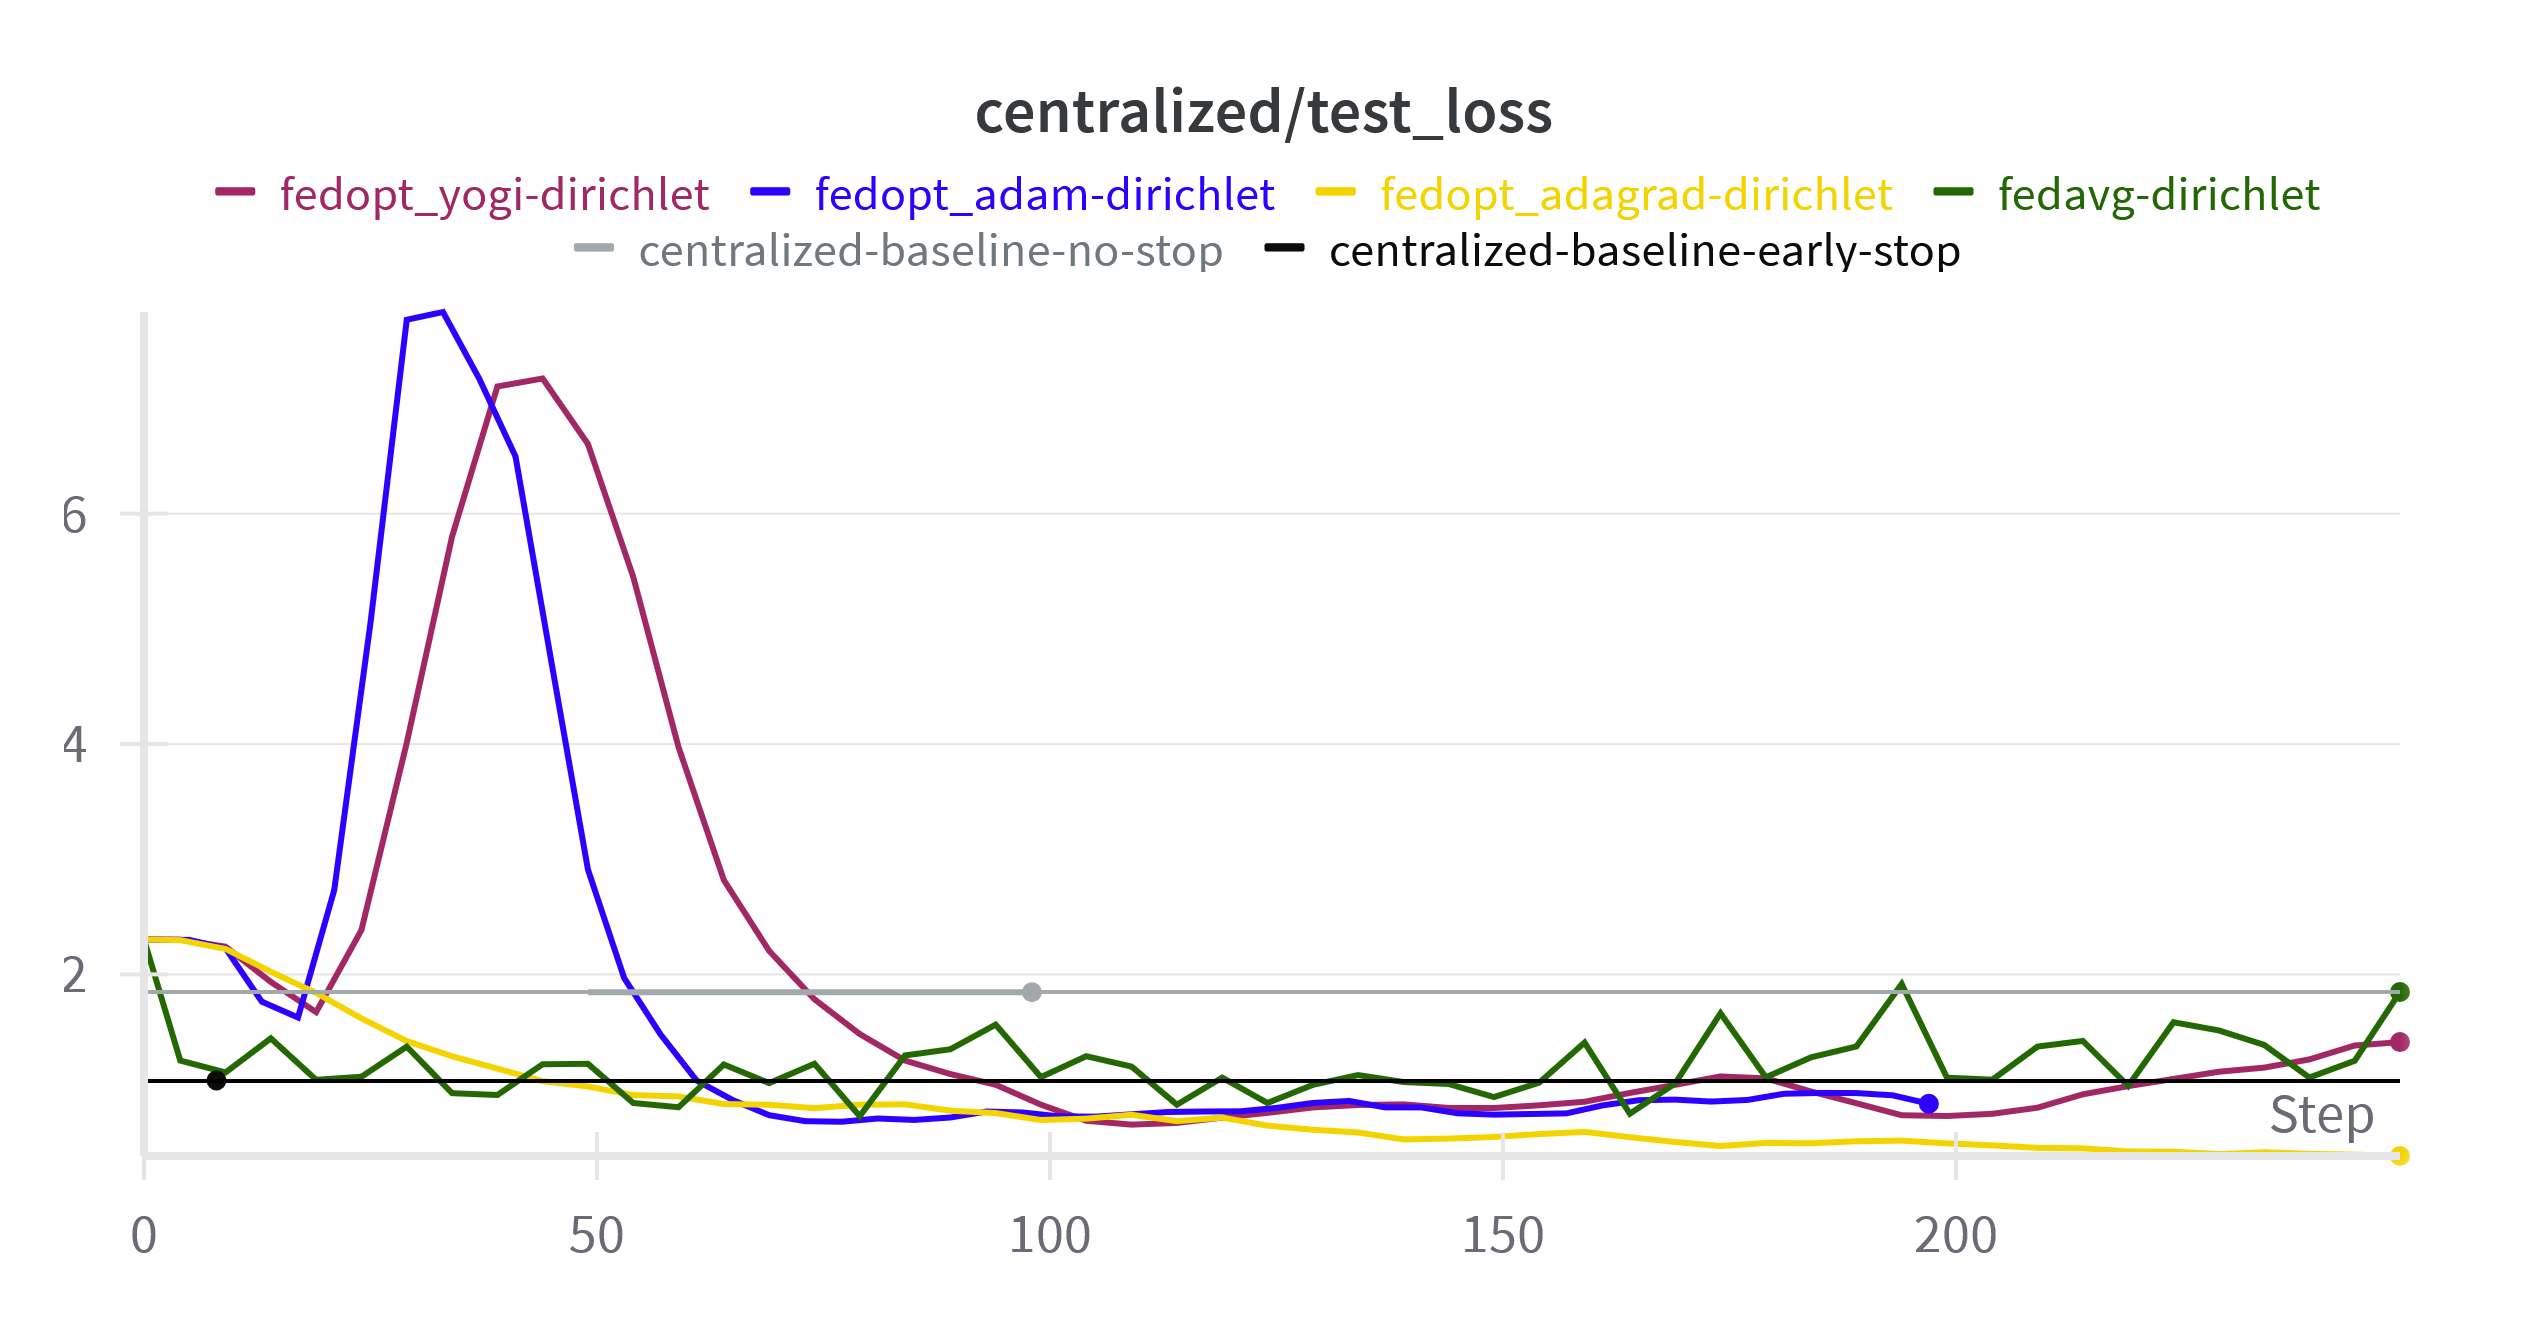
\includegraphics[width=0.48\textwidth]{img/experiment_1/dirichlet_server_test_loss}
        \hfill
        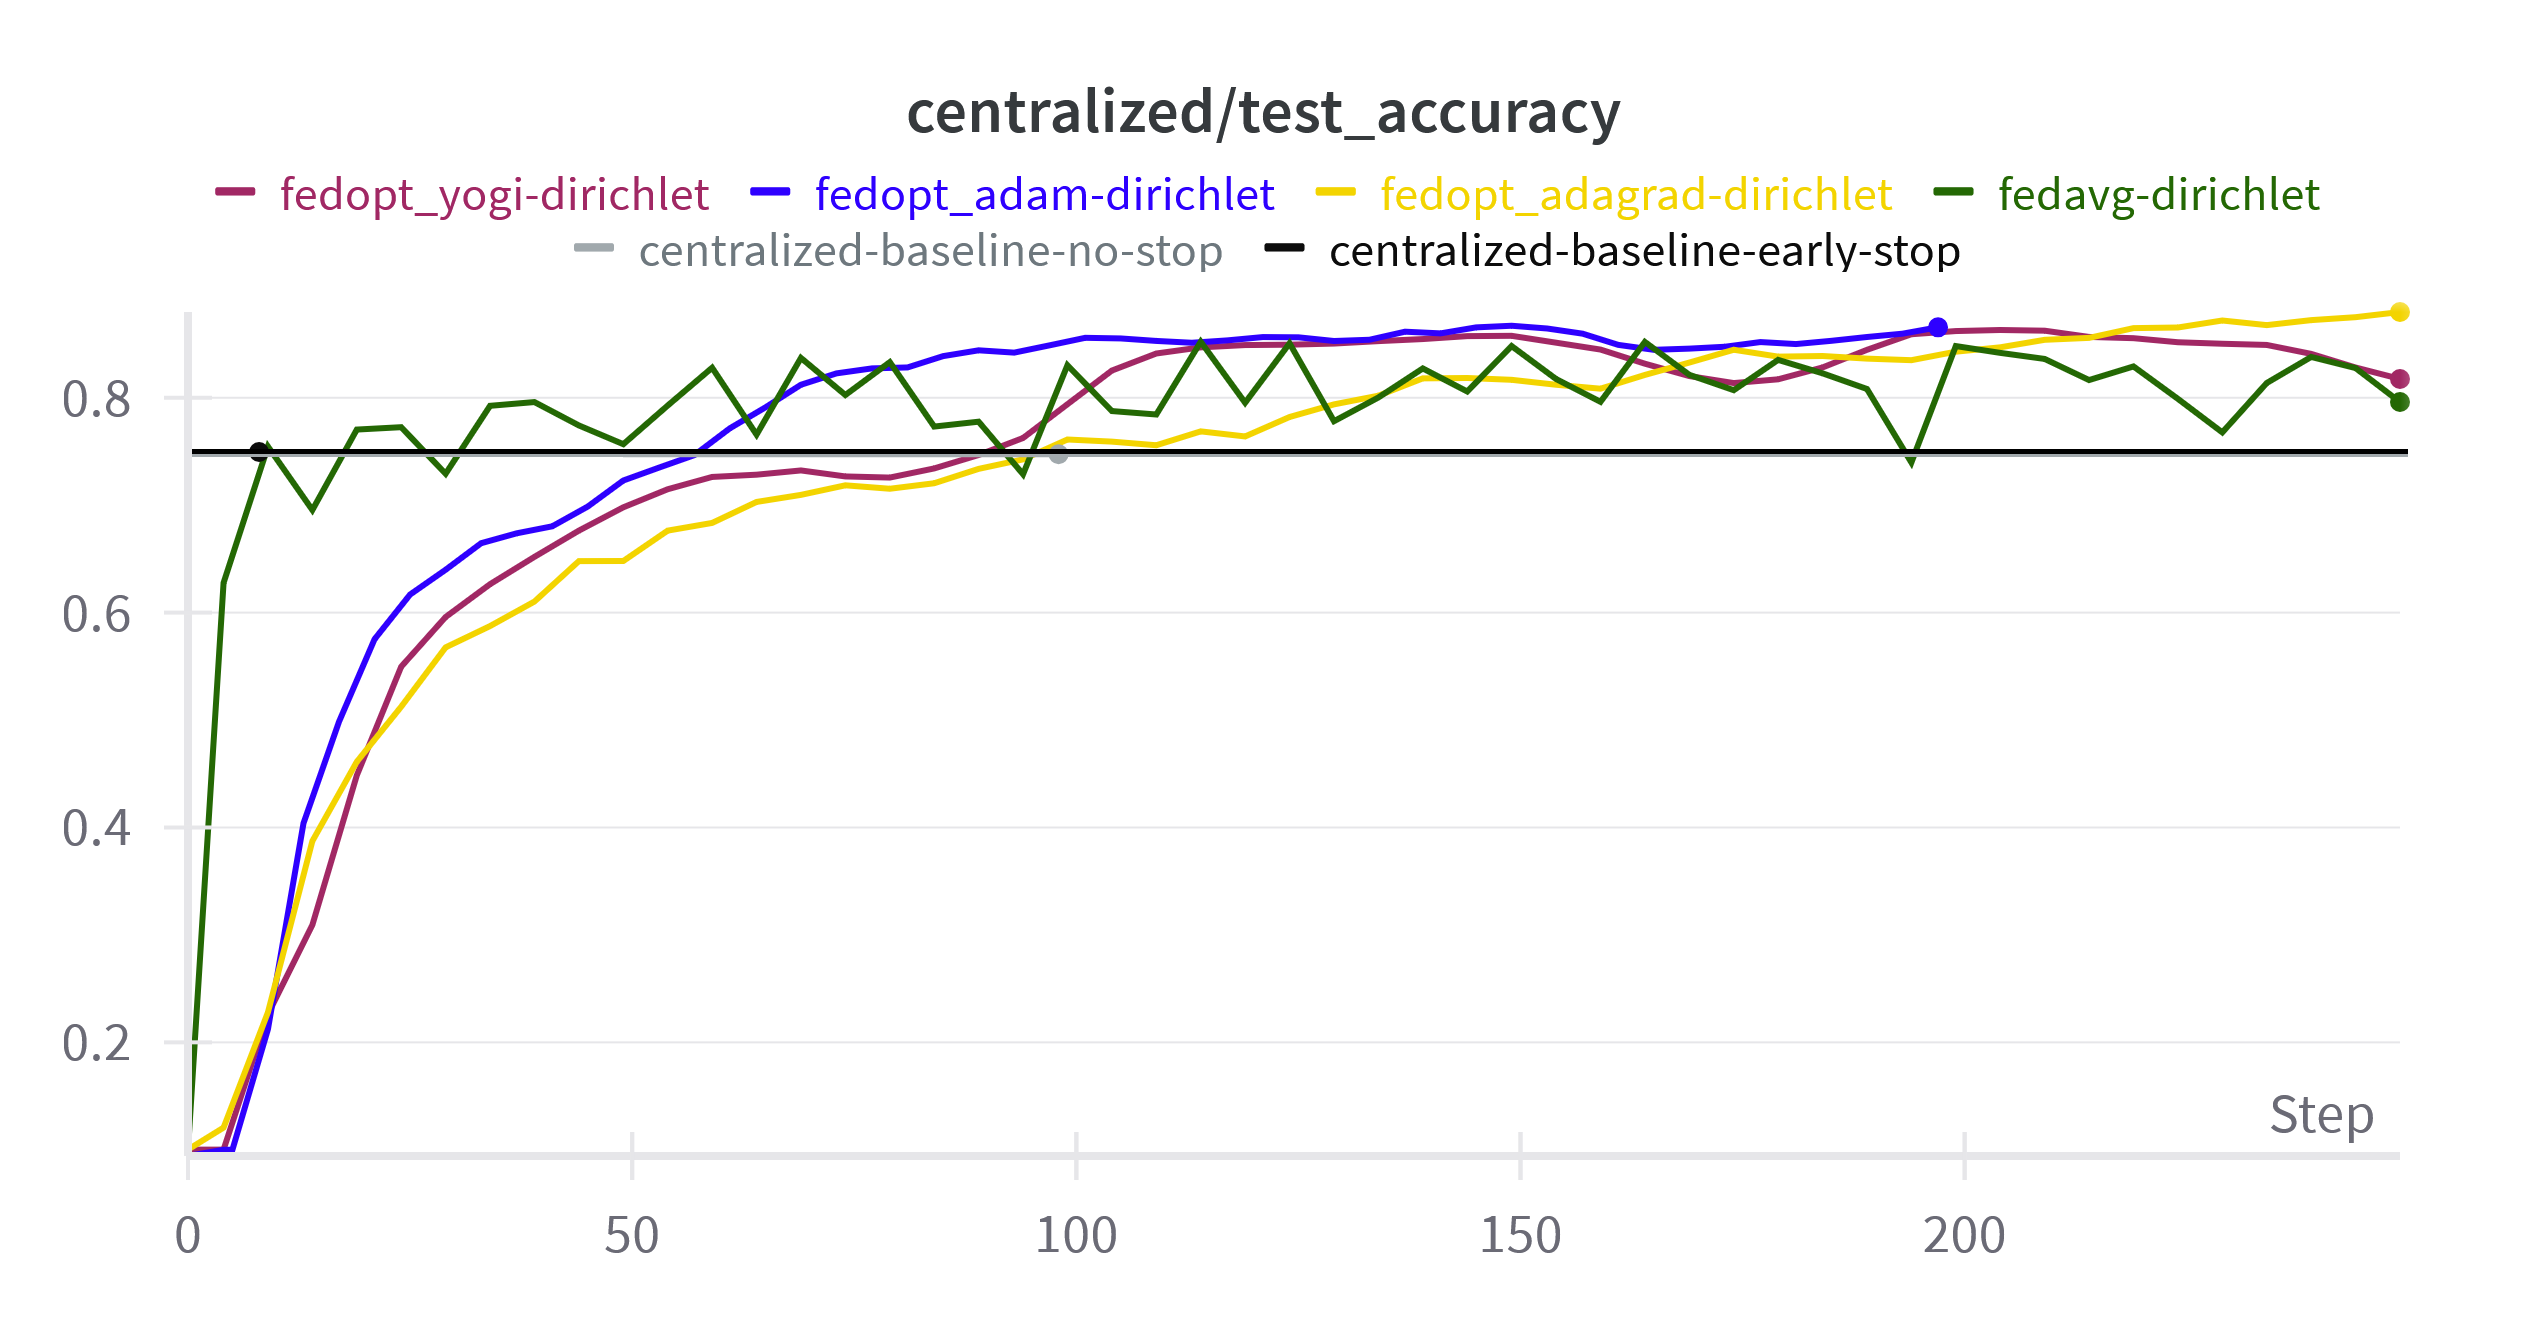
\includegraphics[width=0.48\textwidth]{img/experiment_1/dirichlet_server_test_acc}
        \caption{Global model performance metrics: test loss (left) and accuracy (right) evolution for Dirichlet partitioning}
        \label{fig:dirichlet_global_metrics}
    \end{figure}

    \noindent
    \textbf{Performance Summary}

    Table~\ref{tab:dirichlet_performance} summarizes the final performance metrics for all tested federated optimization strategies under Dirichlet partitioning. The results reveal the most dramatic performance variations among all tested scenarios, with some algorithms showing exceptional improvement while others struggle significantly under statistical heterogeneity.

    \begin{table}[h]
        \centering
        \caption{Performance comparison of federated optimization strategies under Dirichlet partitioning}
        \label{tab:dirichlet_performance}
        \begin{tabular}{|l|c|c|c|}
            \hline
            \textbf{Strategy} & \textbf{Final Accuracy} & \textbf{Final Loss} & \textbf{Rounds to Converge} \\
            \hline
            FedAvg            & 0.796                   & 1.84                & N/A                         \\
            FedOpt (AdaGrad)  & 0.879                   & 0.42                & 41                          \\
            FedOpt (Adam)     & 0.865                   & 0.87                & 40                          \\
            FedOpt (Yogi)     & 0.796                   & 1.41                & 43                          \\
            \hline
        \end{tabular}
    \end{table}

    The performance analysis for the Dirichlet partitioning scenario underscores the severe challenges posed by statistical heterogeneity. The baseline \texttt{FedAvg} strategy achieves the lowest accuracy (79.6\%) and the highest final loss (1.84), failing to converge effectively within the training horizon. Among the \texttt{FedOpt} variants, \texttt{AdaGrad} delivers the most robust results, achieving the highest final accuracy (87.9\%) and the lowest loss (0.42), demonstrating strong generalization and convergence properties under non-IID conditions. \texttt{Adam} also performs well, reaching 86.5\% accuracy but with a higher final loss (0.87), indicating less stable convergence. In contrast, \texttt{Yogi}, despite being effective in other scenarios, struggles under Dirichlet partitioning, matching \texttt{FedAvg} in accuracy (79.6\%) and converging with a relatively high loss (1.41). These results highlight the sensitivity of optimization strategies to class imbalance and distributional shift, with \texttt{AdaGrad} emerging as the most effective optimizer in this heterogeneous setting.

    \subsection{Experiment 2: Full Participation Setting}
    \label{subsec:experiment2}

    The core idea of the experiment is to simulate federated learning with full client participation (\texttt{fraction\_fit = 1.0}), while introducing variability in local training duration across clients to mimic real-world heterogeneity. Each client trains independently for a different number of epochs before synchronization, simulating a semi-asynchronous environment. This approach aims to explore how differing local compute capacities (e.g., CPU vs GPU) affect model convergence and system dynamics under full participation.

    To simulate the idea of different devices training their data, we setup 3 different clients that will train their data per round as follows:
    \begin{itemize}
        \item the first client will train their samples for a number of epochs from the distribution $\mathcal{N}(5, 1)$ (integer approximation).
        \item the second client will train their samples for a number of epochs from the distribution $\mathcal{N}(10, 1)$ (integer approximation).
        \item the third client will train their samples for a number of epochs from the distribution $\mathcal{N}(15, 1)$ (integer approximation).
    \end{itemize}

    Beside this setup, in our experiments we will variate the federated aggregation strategy (between FedAvg - Section \ref{subsec:fedavg}, FedOpt with Adam - Section \ref{subsec:fedopt}, and WeightedFedAvg - Section \ref{subsec:weighted-fedavg}) and the partitioning strategy (between IID, Dirichlet with $\alpha = 0.5$, Dirichlet with $\alpha = 0.1$, and Pathologic, all presented in Section \ref{subsec:partitioning}). The fixed variables for our experiemnts are the following: \texttt{batch\_size per client: 512}, \texttt{learning\_rate per client: 0.001}, \texttt{optimizer per client: adam}, \texttt{fraction\_fit: 1}, \texttt{num\_server\_rounds: 15}, \texttt{learning\_rate server: 0.01}.

    \subsubsection{Centralized Results vs Individual Clients Results across Experiments}
    In this subsection of the results (Figures \ref{fig:exp2-fedavg-iid}, \ref{fig:exp2-fedavg-dirichlet}, \ref{fig:exp2-fedavg-pathological}, \ref{fig:exp2-fedavg-dirichlet-skewed}, \ref{fig:exp2-fedopt-iid}, \ref{fig:exp2-fedopt-dirichlet}, \ref{fig:exp2-fedopt-pathological}, \ref{fig:exp2-fedopt-dirichlet-skewed}, \ref{fig:exp2-weightedfedavg-iid}, \ref{fig:exp2-weightedfedavg-dirichlet}, \ref{fig:exp2-weightedfedavg-pathological}, \ref{fig:exp2-weightedfedavg-dirichlet-skewed}), we plot how the losses and the accuracies evolve over time between each client and the server in each federated learning setup. We compare those with the baseline result (from Section \ref{subsec:baseline_results}). In each figure, there are 3 plots:
    \begin{itemize}
        \item in the first plot (left) the training loss of each client is compared to the centralized test loss,
        \item in the second plot (center) the test loss of each client is compared to the centralized test loss,
        \item in the third plot (right) the test accuracy of each client is compared to the centralized accuracy.
    \end{itemize}

    \begin{figure}[h!]
        \centering
        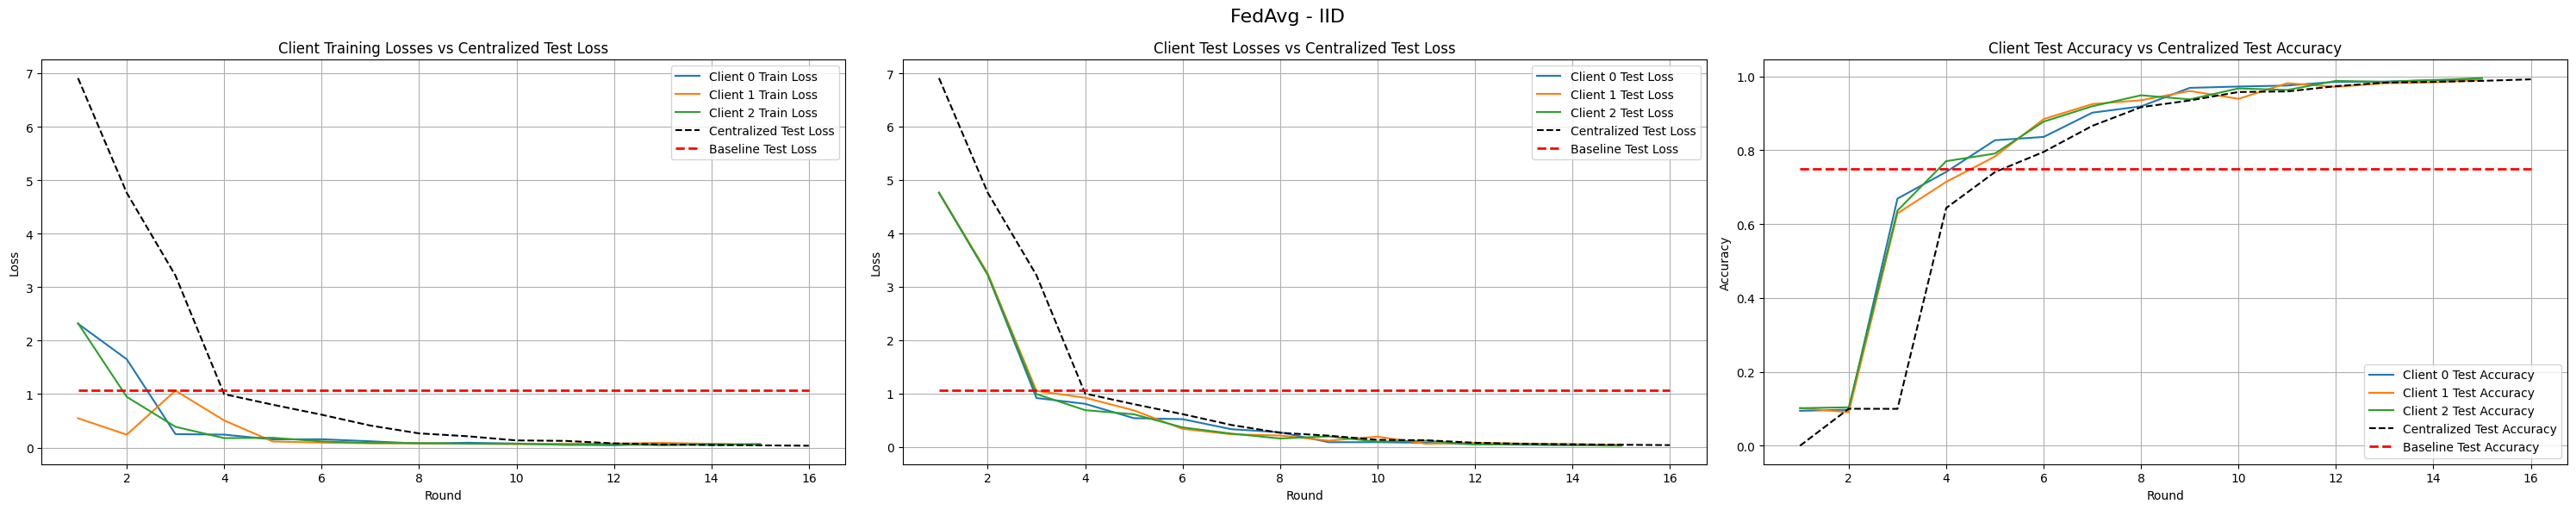
\includegraphics[width=1\linewidth]{img/experiment_2/fedavg-iid}
        \caption{Results for FedAvg aggregating strategy and IID partitioning strategy.}
        \label{fig:exp2-fedavg-iid}
    \end{figure}

    \begin{figure}[h!]
        \centering
        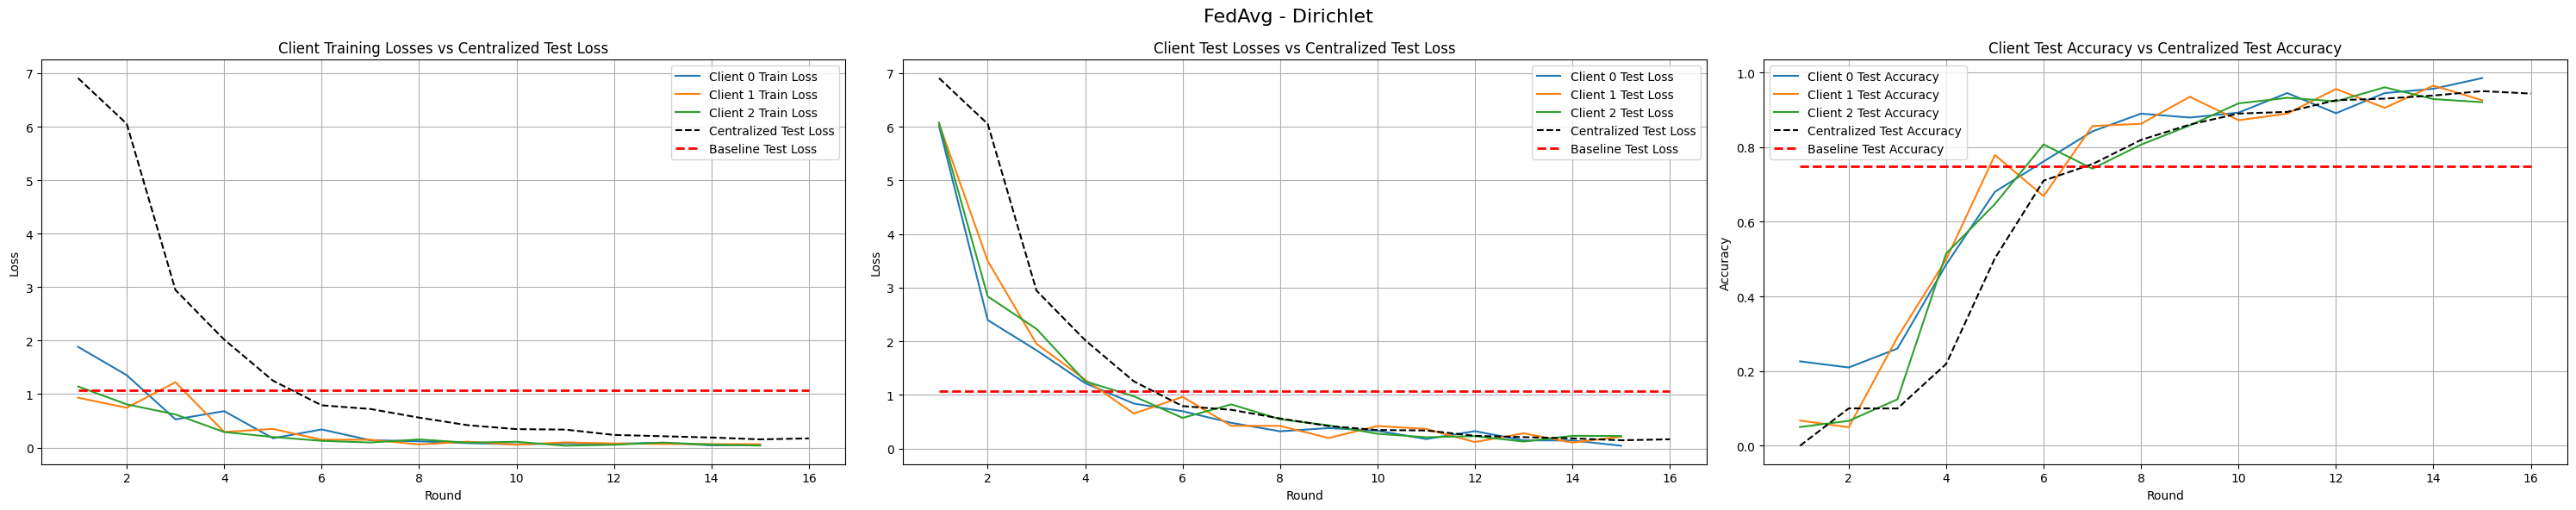
\includegraphics[width=1\linewidth]{img/experiment_2/fedavg-dirichlet}
        \caption{Results for FedAvg aggregating strategy and Dirichlet partitioning strategy.}
        \label{fig:exp2-fedavg-dirichlet}
    \end{figure}

    \begin{figure}[h!]
        \centering
        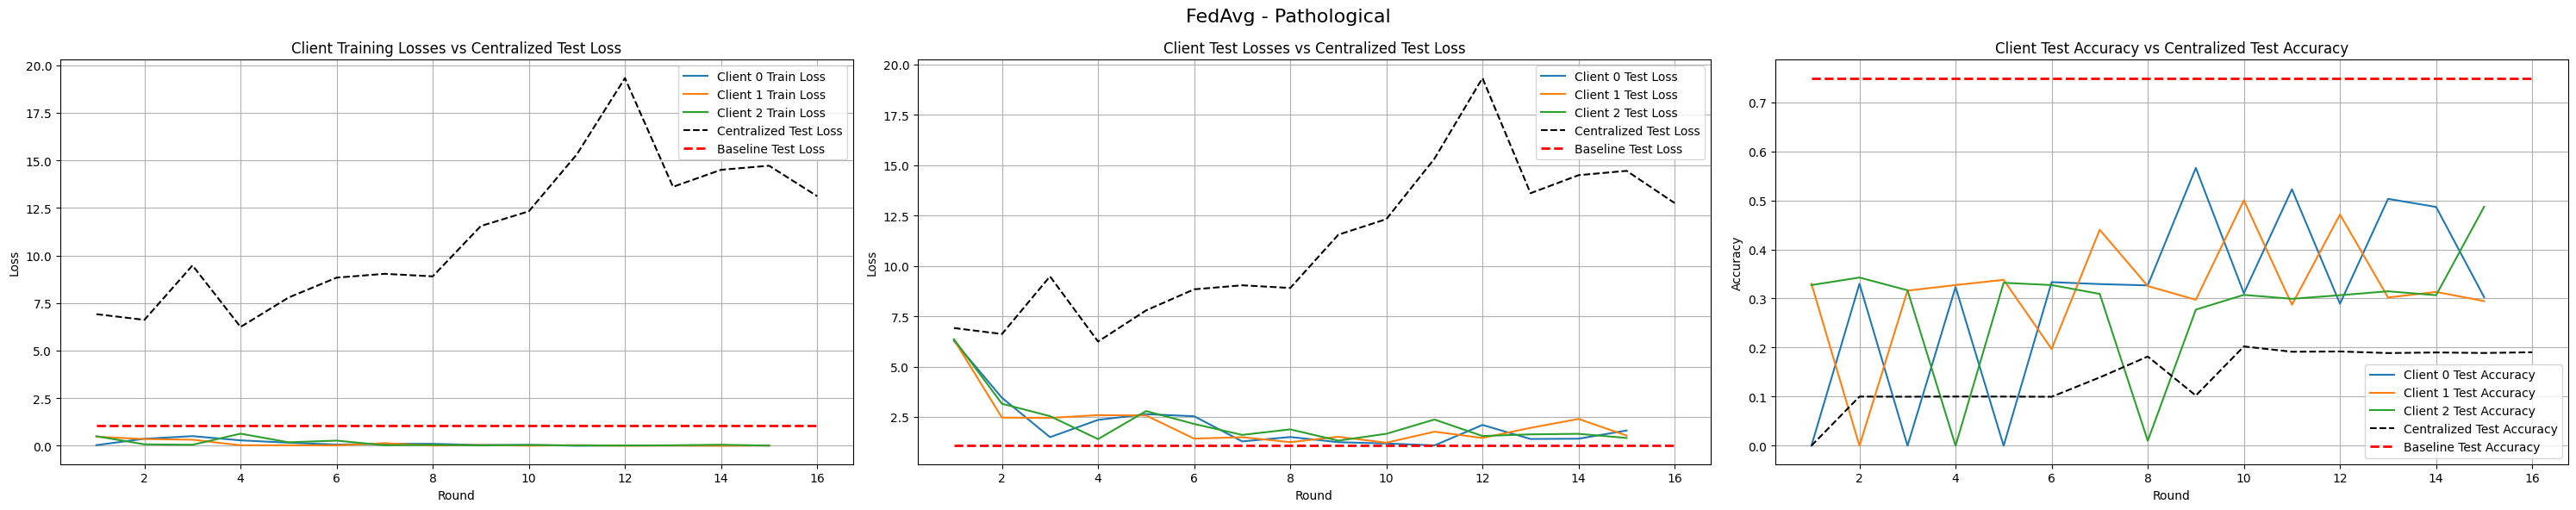
\includegraphics[width=1\linewidth]{img/experiment_2/fedavg-pathological}
        \caption{Results for FedAvg aggregating strategy and Pathological partitioning strategy.}
        \label{fig:exp2-fedavg-pathological}
    \end{figure}

    \begin{figure}[h!]
        \centering
        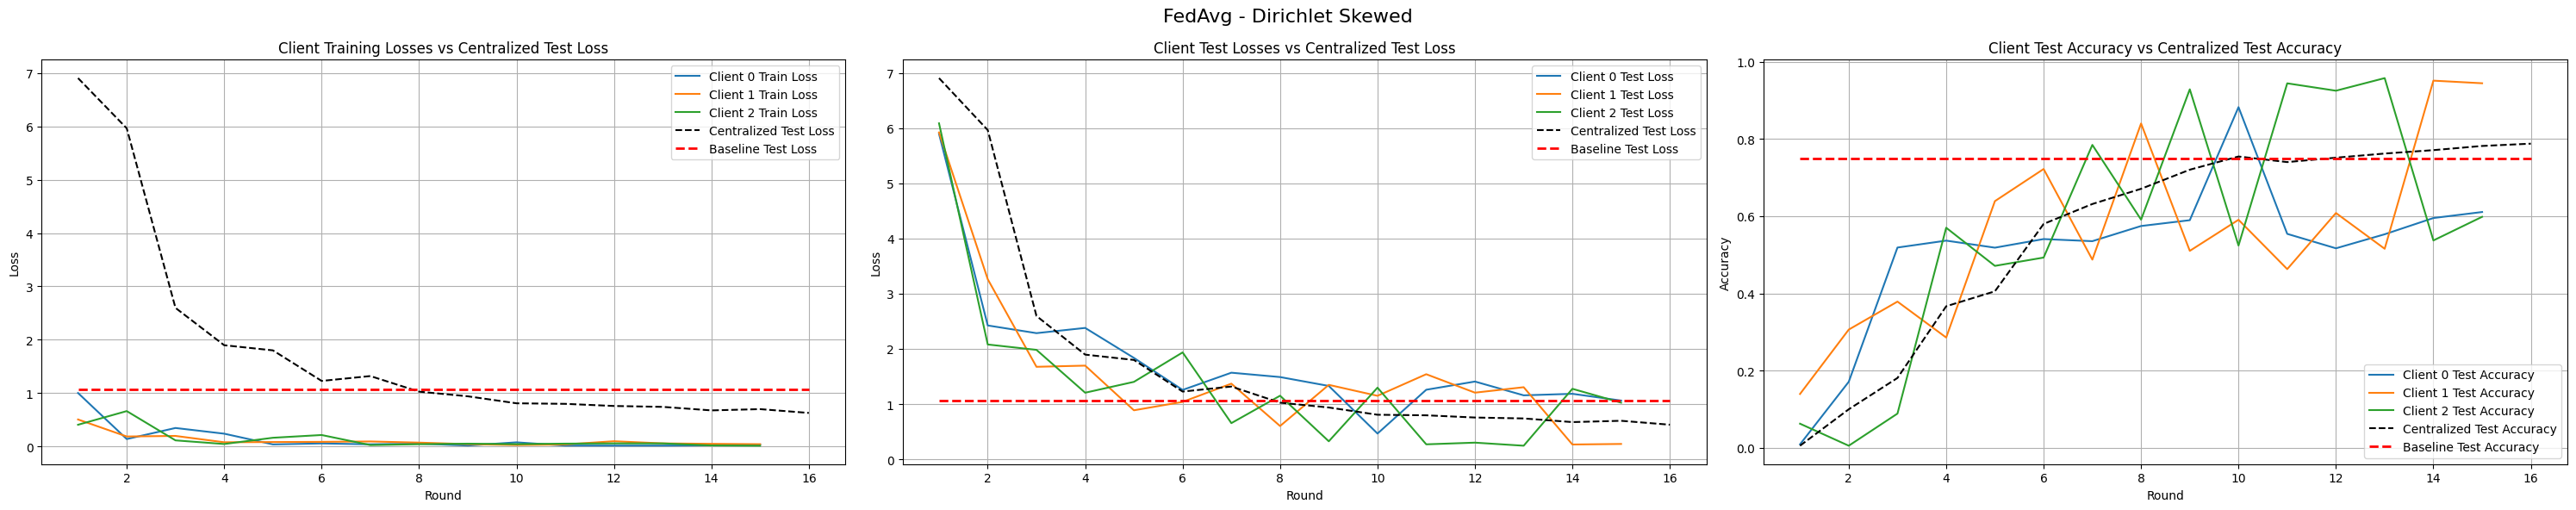
\includegraphics[width=1\linewidth]{img/experiment_2/fedavg-dirichlet-skewed}
        \caption{Results for FedAvg aggregating strategy and Dirichlet Skewed partitioning strategy.}
        \label{fig:exp2-fedavg-dirichlet-skewed}
    \end{figure}

    \begin{figure}[h!]
        \centering
        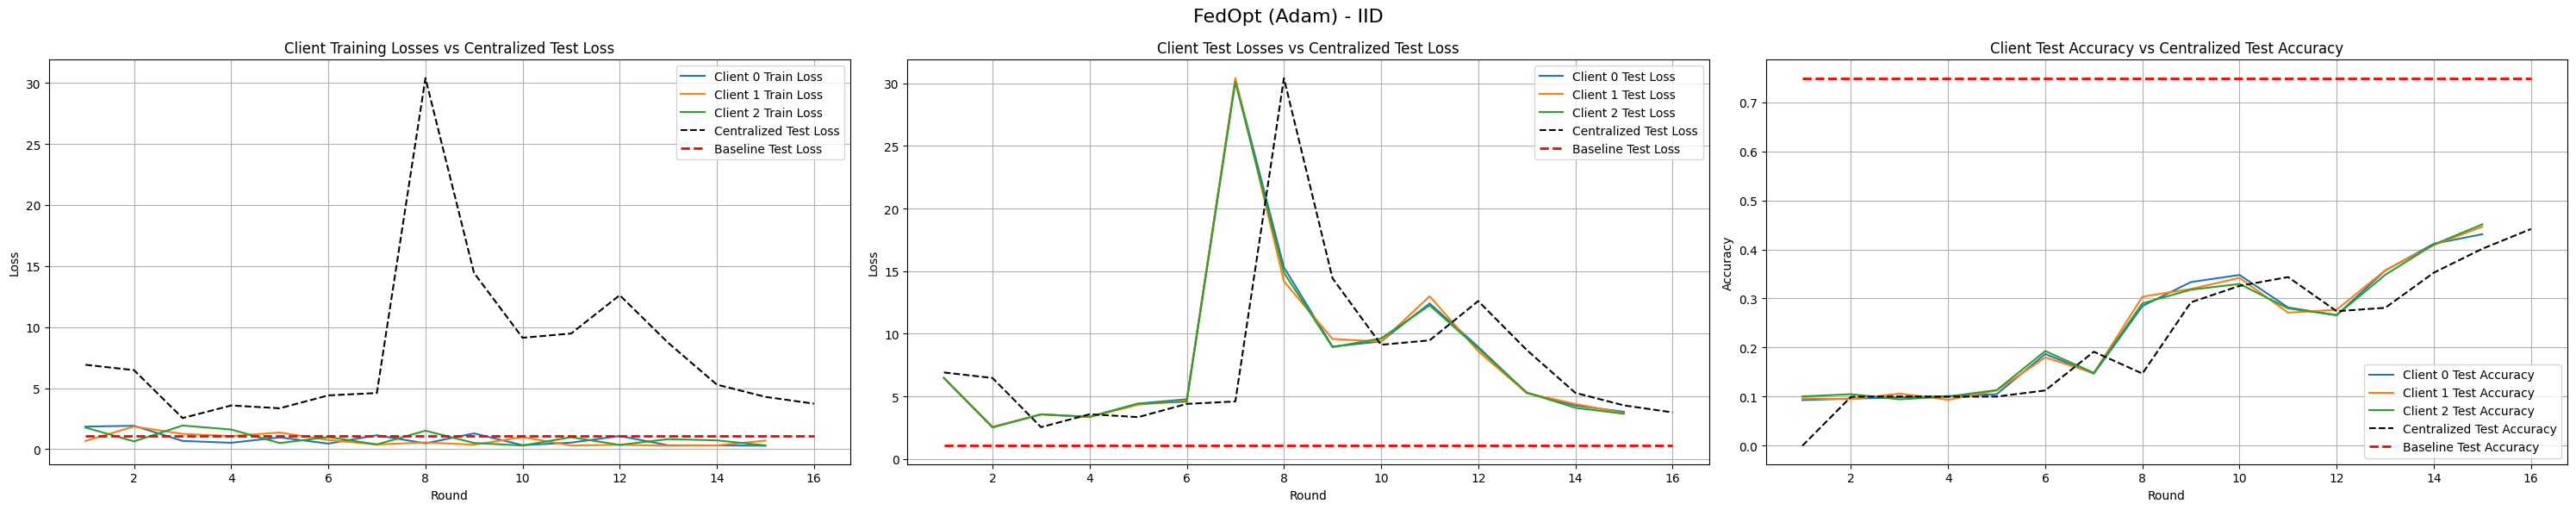
\includegraphics[width=1\linewidth]{img/experiment_2/fedopt-iid}
        \caption{Results for FedOpt (Adam) aggregating strategy and IID partitioning strategy.}
        \label{fig:exp2-fedopt-iid}
    \end{figure}

    \begin{figure}[h!]
        \centering
        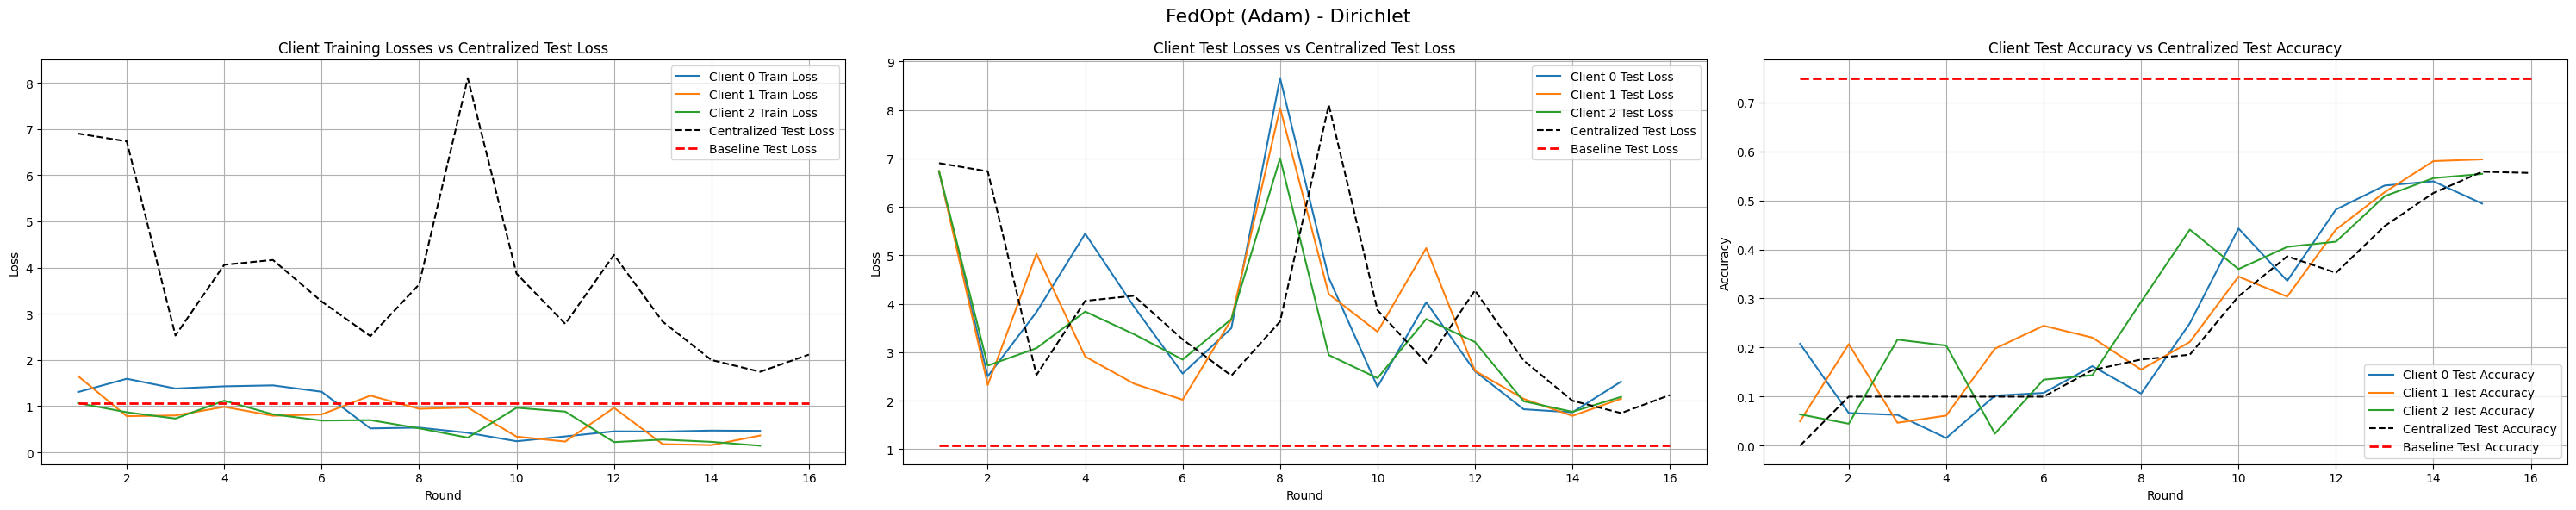
\includegraphics[width=1\linewidth]{img/experiment_2/fedopt-dirichlet}
        \caption{Results for FedOpt (Adam) aggregating strategy and Dirichlet partitioning strategy.}
        \label{fig:exp2-fedopt-dirichlet}
    \end{figure}

    \begin{figure}[h!]
        \centering
        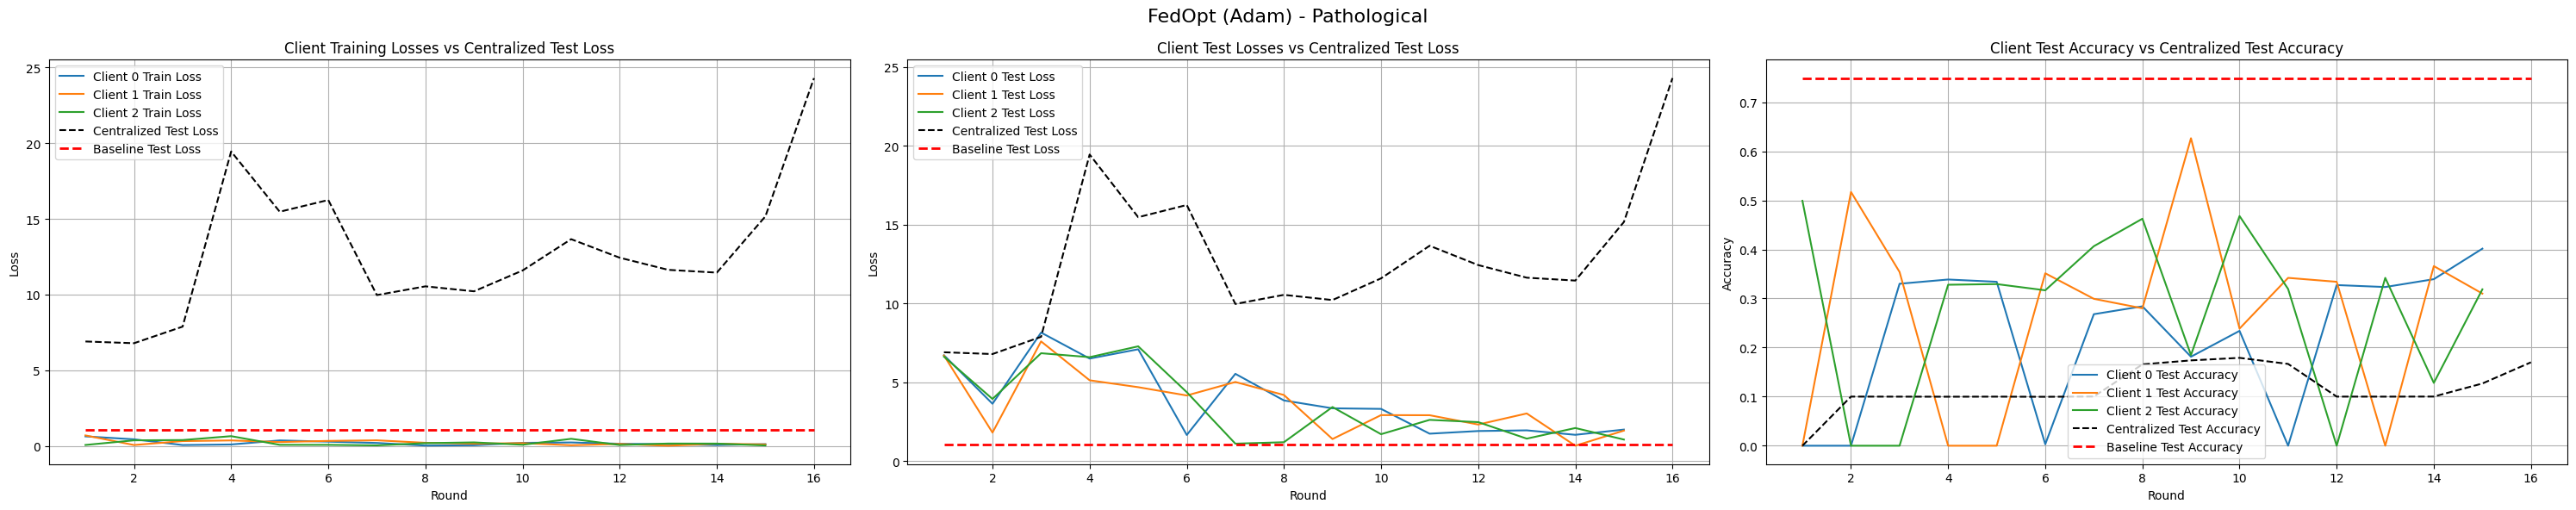
\includegraphics[width=1\linewidth]{img/experiment_2/fedopt-pathological}
        \caption{Results for FedOpt (Adam) aggregating strategy and Pathological partitioning strategy.}
        \label{fig:exp2-fedopt-pathological}
    \end{figure}

    \begin{figure}[h!]
        \centering
        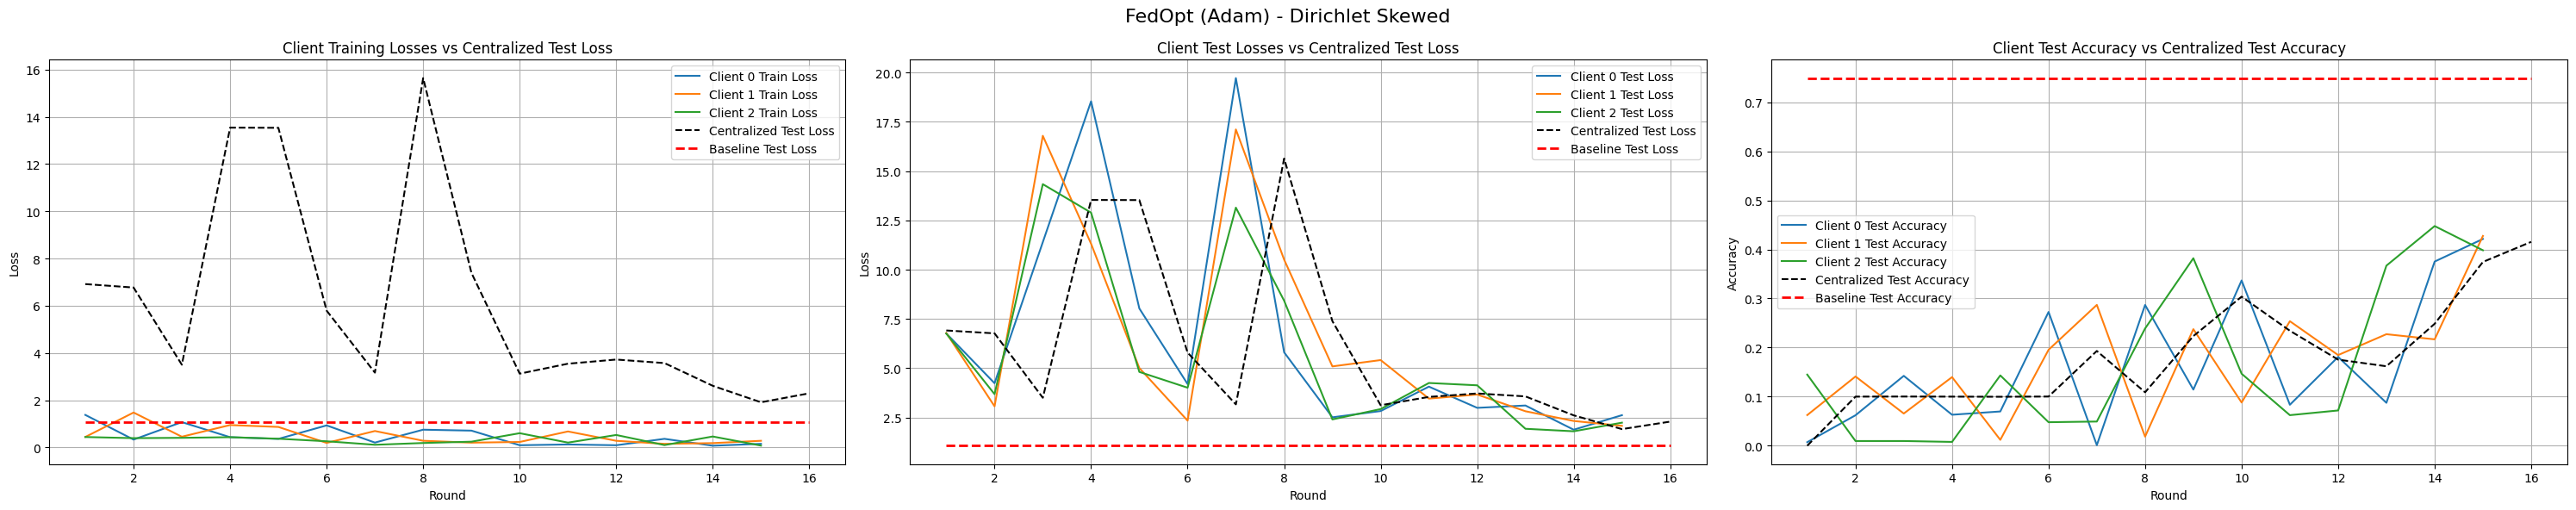
\includegraphics[width=1\linewidth]{img/experiment_2/fedopt-dirichlet-skewed}
        \caption{Results for FedOpt (Adam) aggregating strategy and Dirichlet Skewed partitioning strategy.}
        \label{fig:exp2-fedopt-dirichlet-skewed}
    \end{figure}

    \begin{figure}[h!]
        \centering
        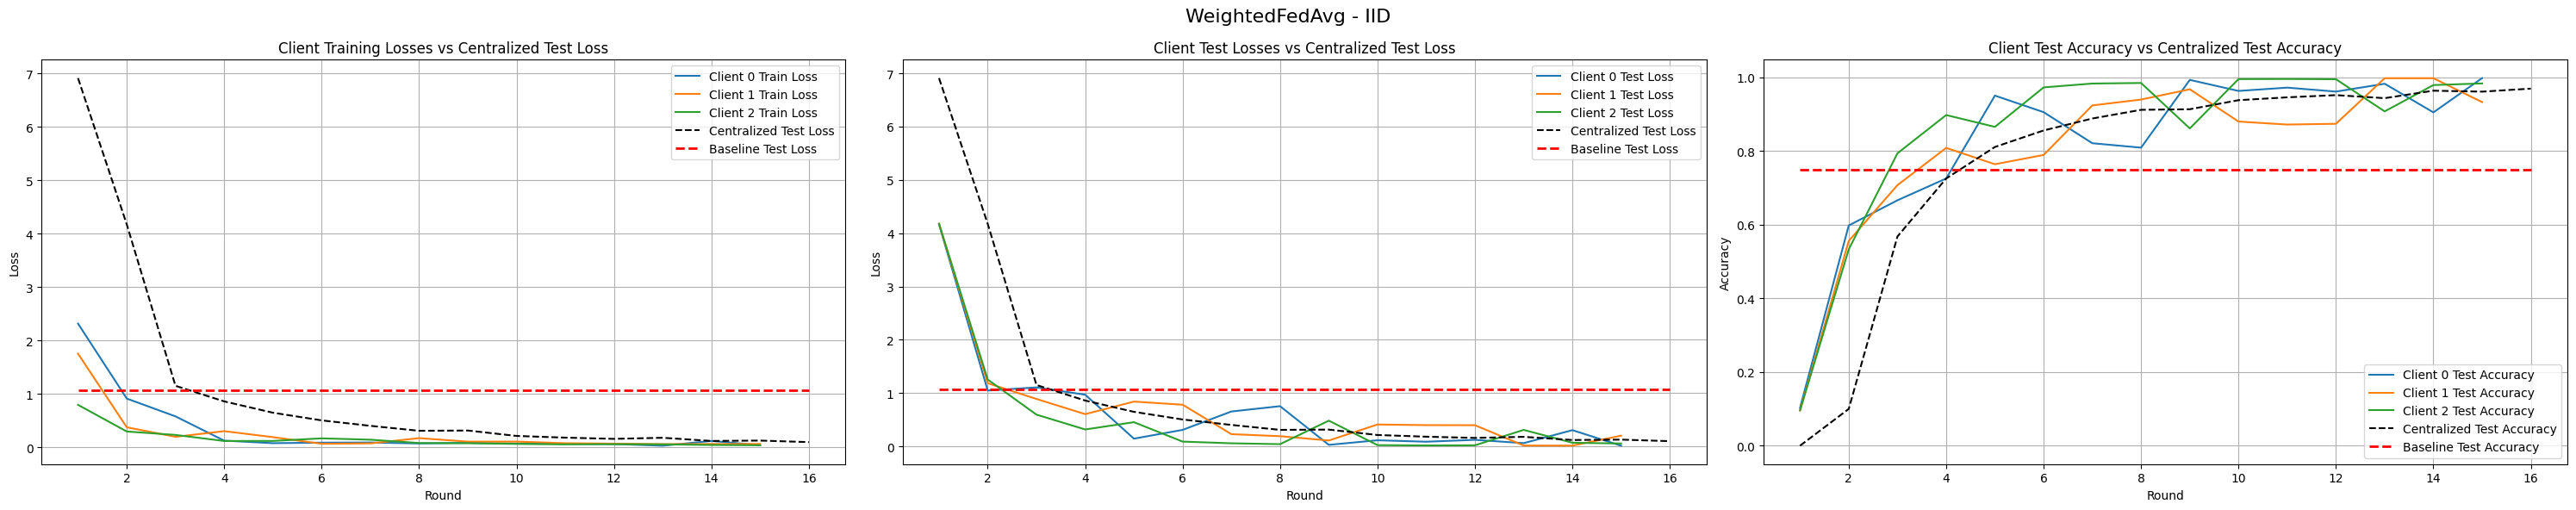
\includegraphics[width=1\linewidth]{img/experiment_2/weightedfedavg-iid}
        \caption{Results for Weighted-FedAvg aggregating strategy and IID partitioning strategy.}
        \label{fig:exp2-weightedfedavg-iid}
    \end{figure}

    \begin{figure}[h!]
        \centering
        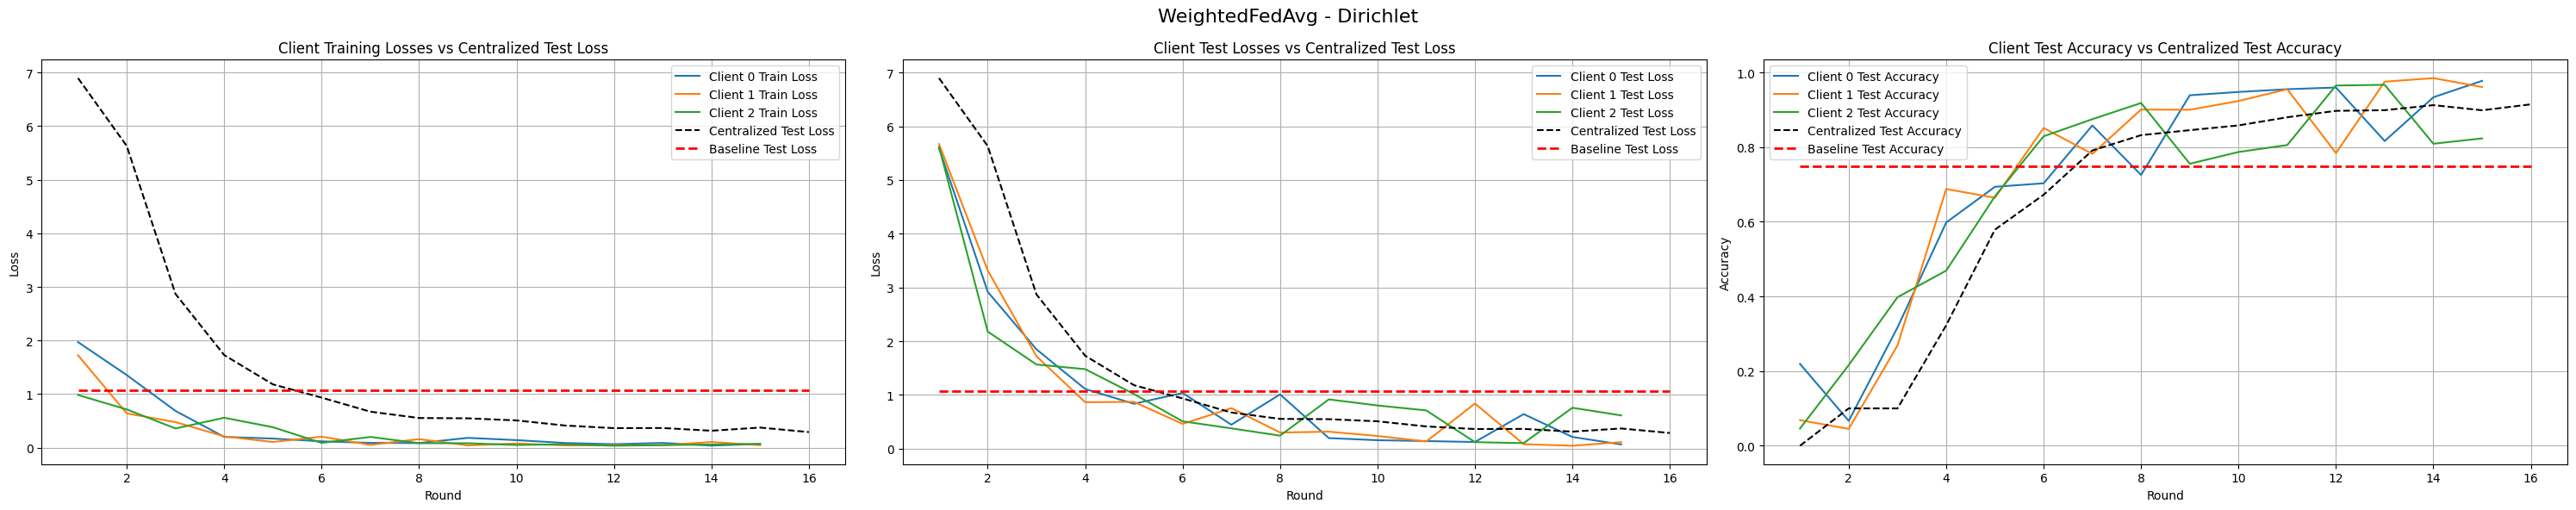
\includegraphics[width=1\linewidth]{img/experiment_2/weightedfedavg-dirichlet}
        \caption{Results for Weighted-FedAvg aggregating strategy and Dirichlet partitioning strategy.}
        \label{fig:exp2-weightedfedavg-dirichlet}
    \end{figure}

    \begin{figure}[h!]
        \centering
        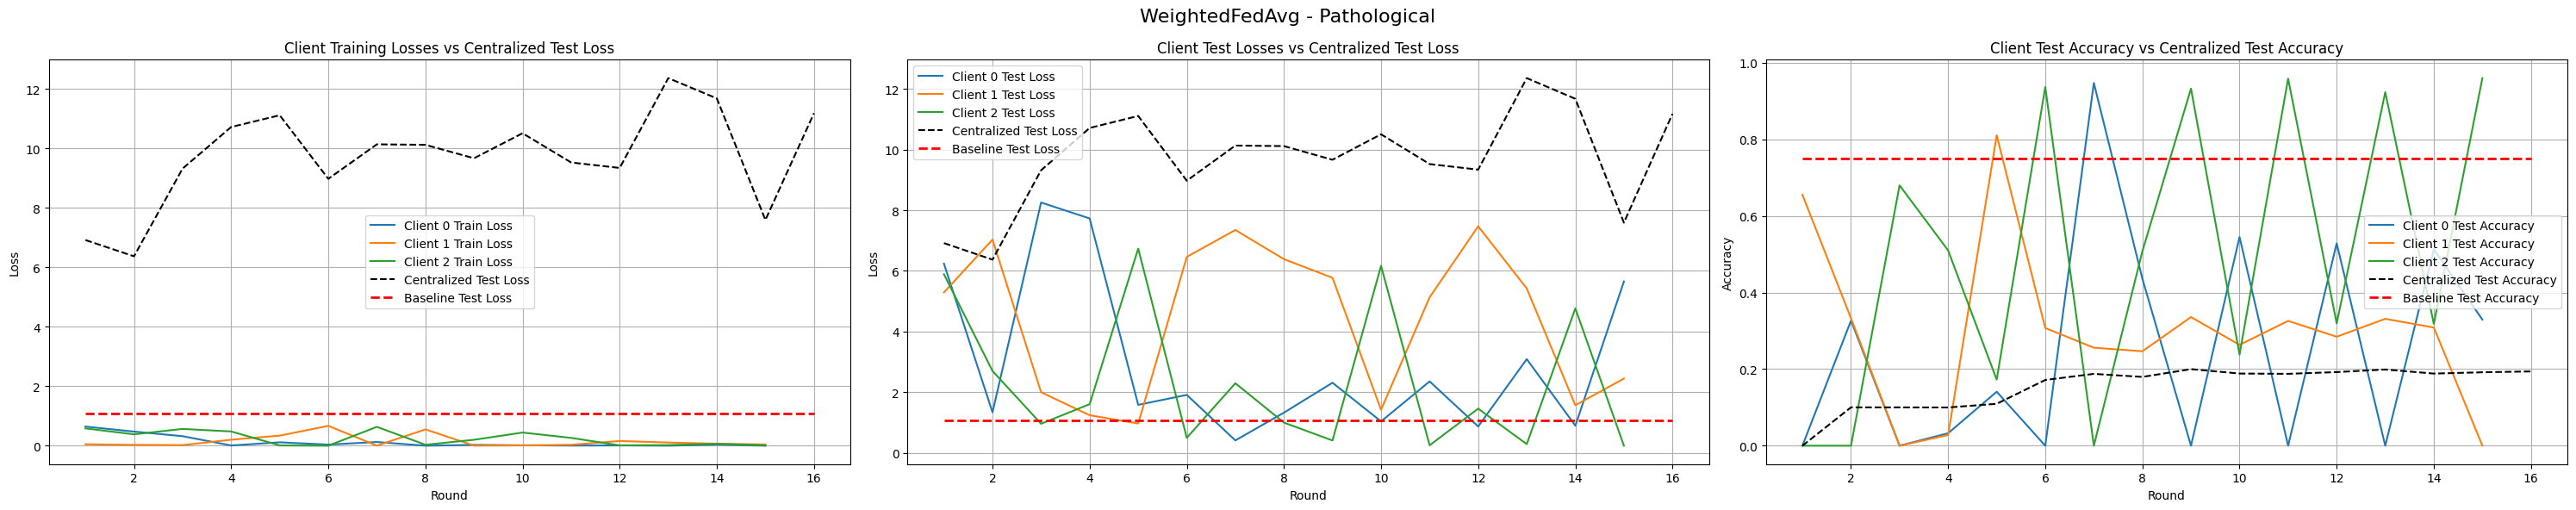
\includegraphics[width=1\linewidth]{img/experiment_2/weightedfedavg-pathological}
        \caption{Results for Weighted-FedAvg aggregating strategy and Pathological partitioning strategy.}
        \label{fig:exp2-weightedfedavg-pathological}
    \end{figure}

    \begin{figure}[h!]
        \centering
        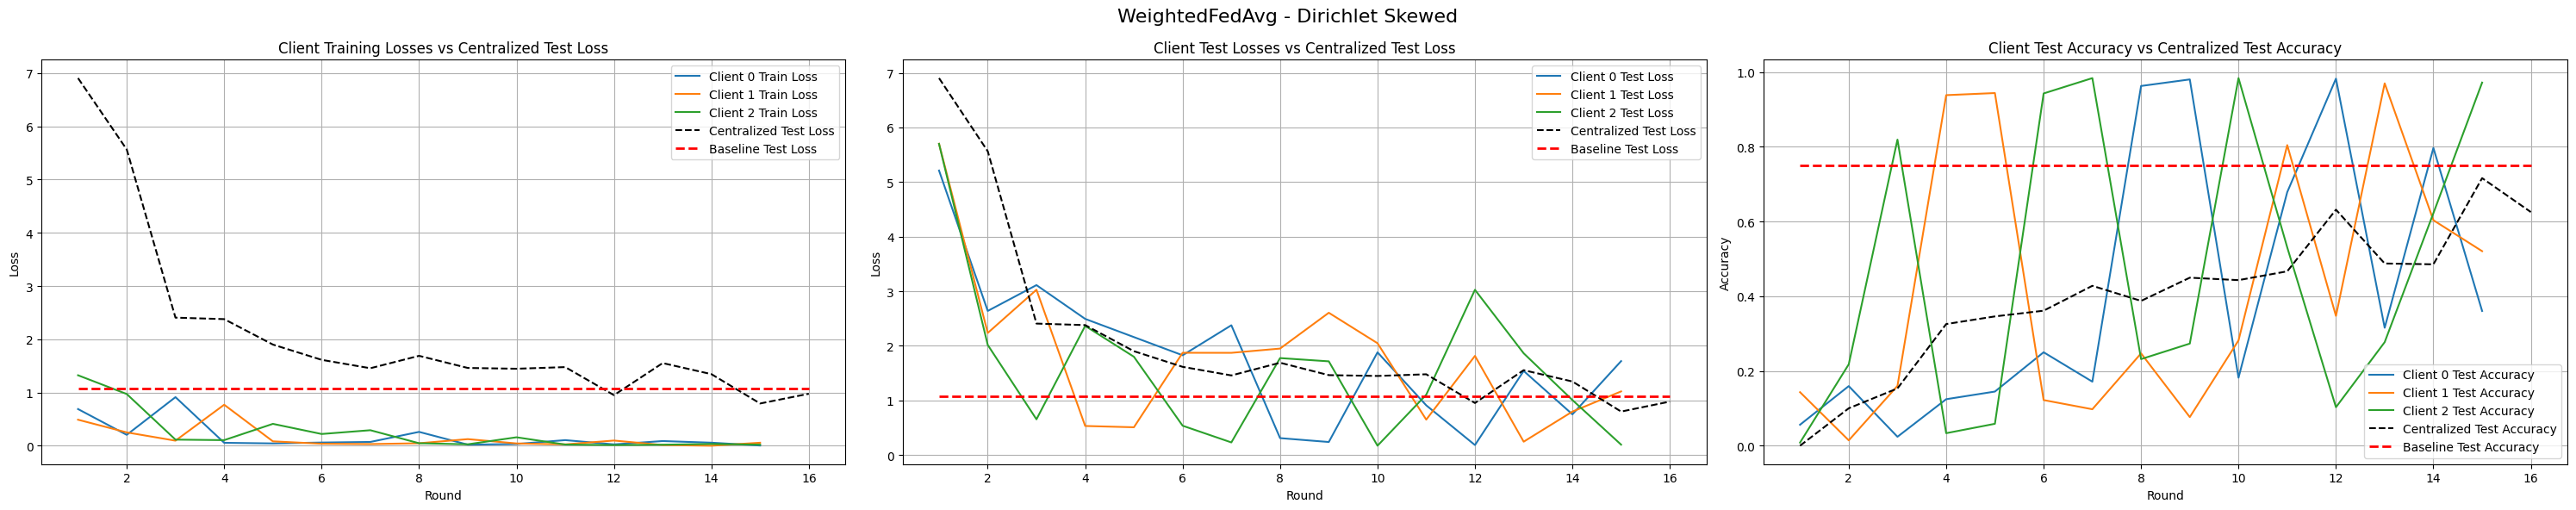
\includegraphics[width=1\linewidth]{img/experiment_2/weightedfedavg-dirichlet-skewed}
        \caption{Results for Weighted-FedAvg aggregating strategy and Dirichlet Skewed partitioning strategy.}
        \label{fig:exp2-weightedfedavg-dirichlet-skewed}
    \end{figure}

    \subsubsection{Results Comparison between Aggregation Strategies across Partition Strategies}
    In this subsection of the results (Figures \ref{fig:exp2-iid-comparison}, \ref{fig:exp2-dirichlet-comparison}, \ref{fig:exp2-pathological-comparison}, \ref{fig:exp2-dirichlet-skewed-comparison}), we plot how different the test losses and the test accuracies of each aggregation strategy in comparison with the test loss and test accuracy from the baseline, based on various partition strategies. In each figure, there are 2 plots:
    \begin{itemize}
        \item the first plot (left) showcases the test loss across rounds for each aggregation strategy compared to the baseline,
        \item the second plot (right) showcases the test accuracies across rounds for each aggregation strategy compared to the baseline.
    \end{itemize}

    \begin{figure}[h!]
        \centering
        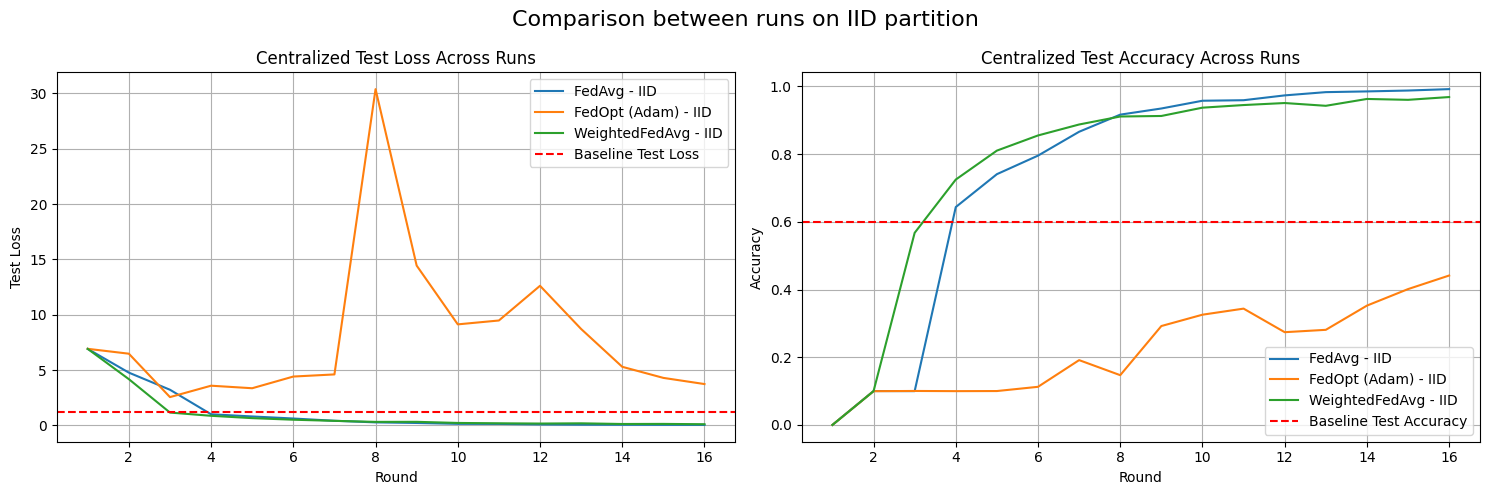
\includegraphics[width=1\linewidth]{img/experiment_2/iid-comparison}
        \caption{Comparison between various aggregation strategy on IID partition strategy.}
        \label{fig:exp2-iid-comparison}
    \end{figure}

    \begin{figure}[h!]
        \centering
        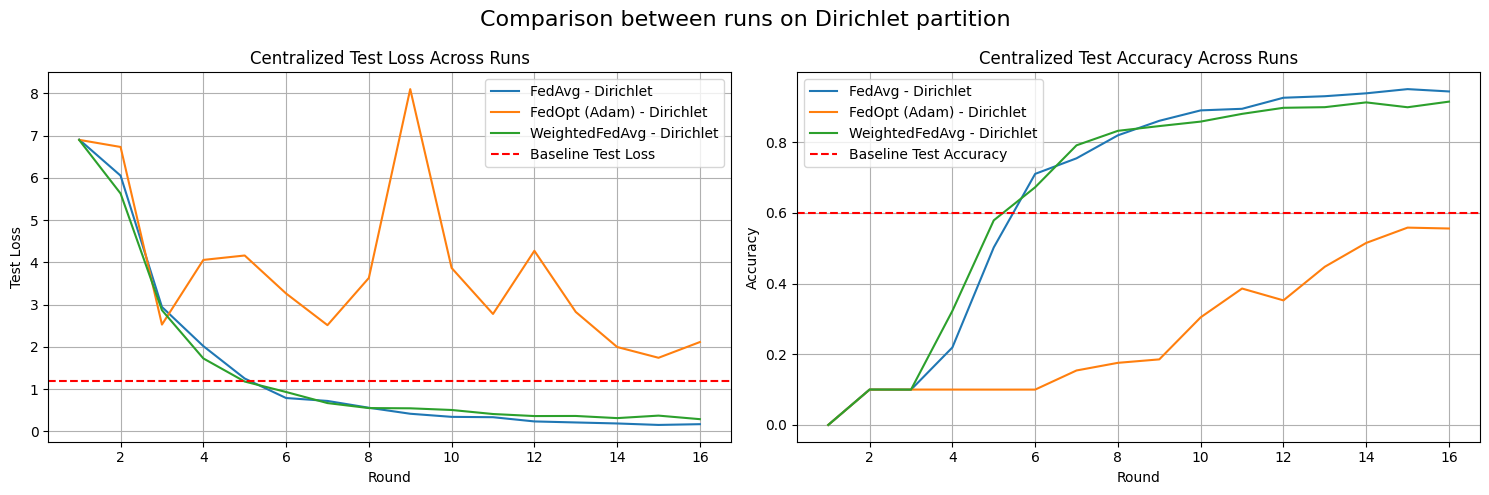
\includegraphics[width=1\linewidth]{img/experiment_2/dirichlet-comparison}
        \caption{Comparison between various aggregation strategy on Dirichlet partition strategy.}
        \label{fig:exp2-dirichlet-comparison}
    \end{figure}

    \begin{figure}[h!]
        \centering
        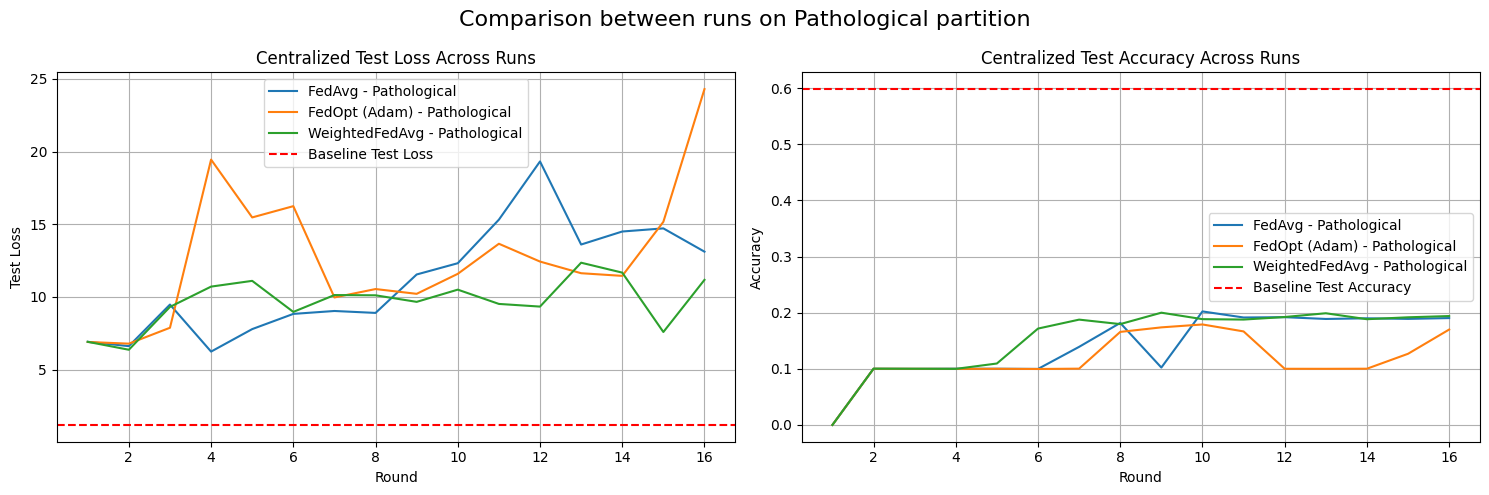
\includegraphics[width=1\linewidth]{img/experiment_2/pathological-comparison}
        \caption{Comparison between various aggregation strategy on Pathological partition strategy.}
        \label{fig:exp2-pathological-comparison}
    \end{figure}

    \begin{figure}[h!]
        \centering
        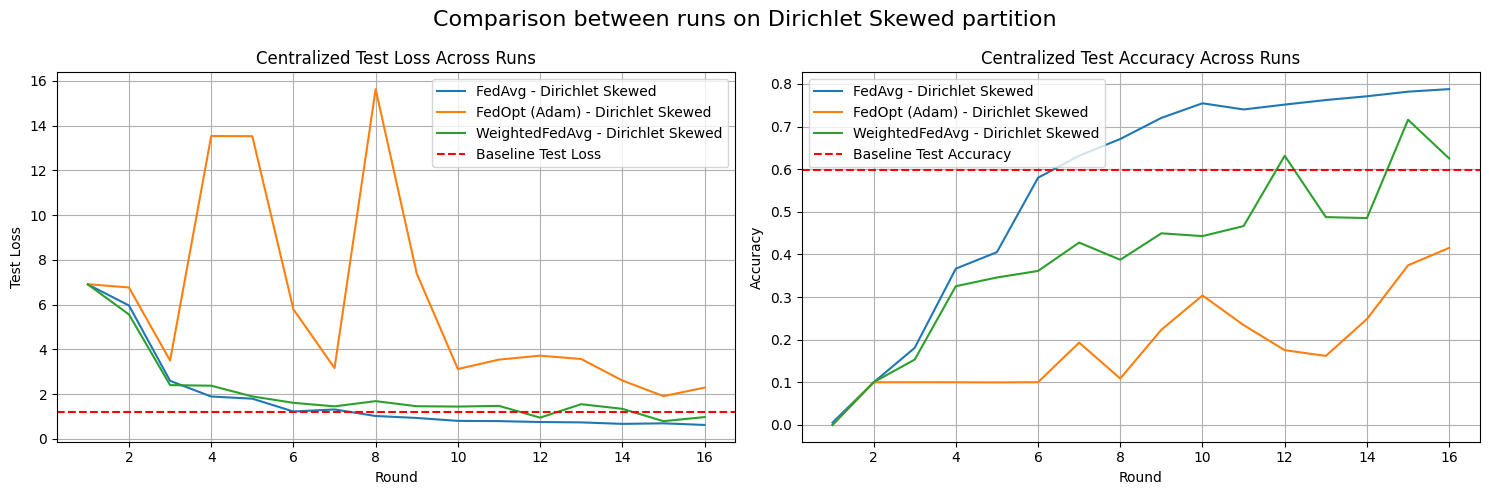
\includegraphics[width=1\linewidth]{img/experiment_2/dirichlet-skewed-comparison}
        \caption{Comparison between various aggregation strategy on Dirichlet Skewed partition strategy.}
        \label{fig:exp2-dirichlet-skewed-comparison}
    \end{figure}

    \subsection{Results Comparison between Partition Strategies across Aggregation Strategies}
    In this subsection of the results (Figures \ref{fig:exp2-fedavg-comparison}, \ref{fig:exp2-fedopt-comparison}, \ref{fig:exp2-weightedfedavg-comparison}), we plot how different the test losses and the test accuracies of each parition strategy in comparison with the test loss and test accuracy from the baseline, based on various aggregation strategies. In each figure, there are 2 plots:
    \begin{itemize}
        \item the first plot (left) showcases the test loss across rounds for each partition strategy compared to the baseline,
        \item the second plot (right) showcases the test accuracies across rounds for each partition strategy compared to the baseline.
    \end{itemize}

    \begin{figure}[h!]
        \centering
        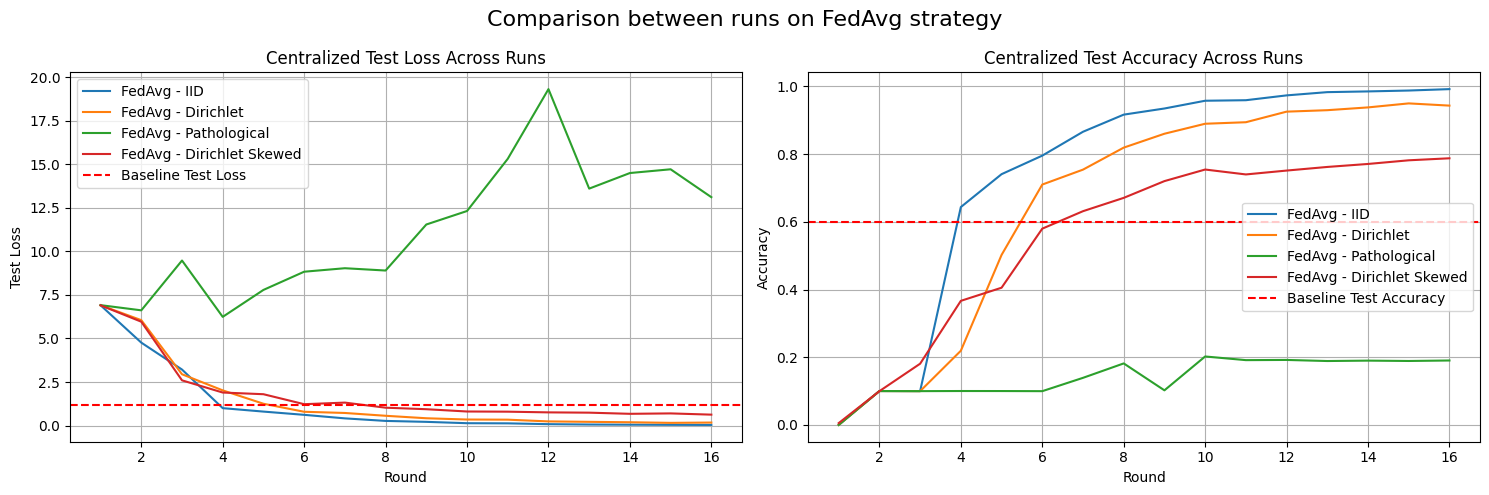
\includegraphics[width=1\linewidth]{img/experiment_2/fedavg-comparison}
        \caption{Comparison between various partition strategy on FedAvg aggregation strategy.}
        \label{fig:exp2-fedavg-comparison}
    \end{figure}

    \begin{figure}[h!]
        \centering
        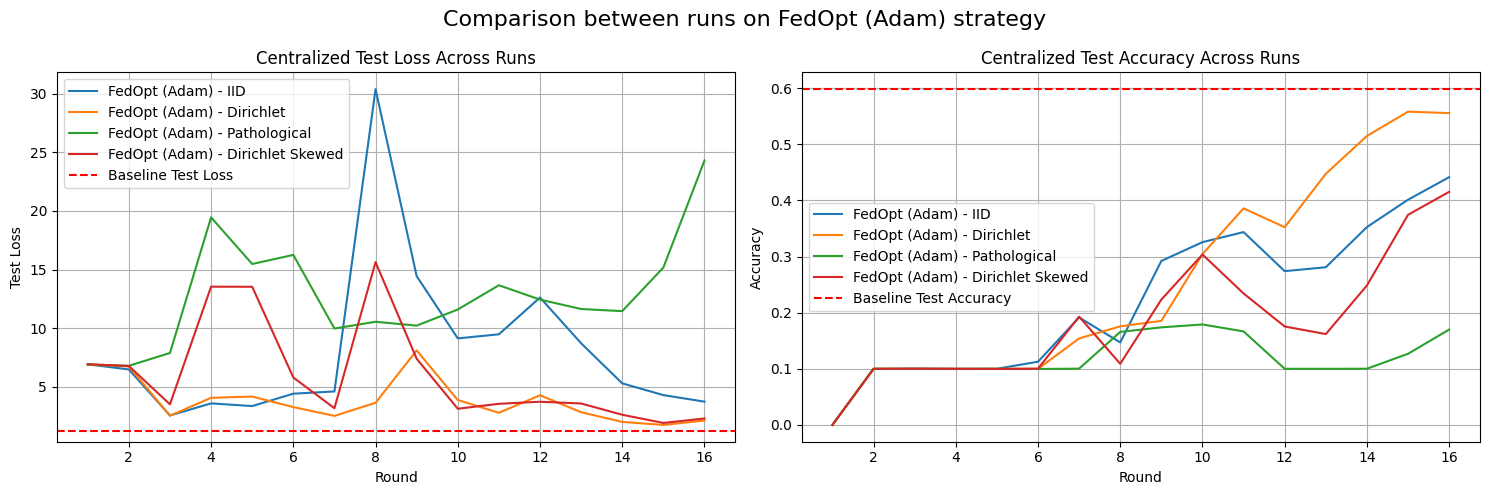
\includegraphics[width=1\linewidth]{img/experiment_2/fedopt-comparison}
        \caption{Comparison between various partition strategy on FedOpt (Adam) aggregation strategy.}
        \label{fig:exp2-fedopt-comparison}
    \end{figure}

    \begin{figure}[h!]
        \centering
        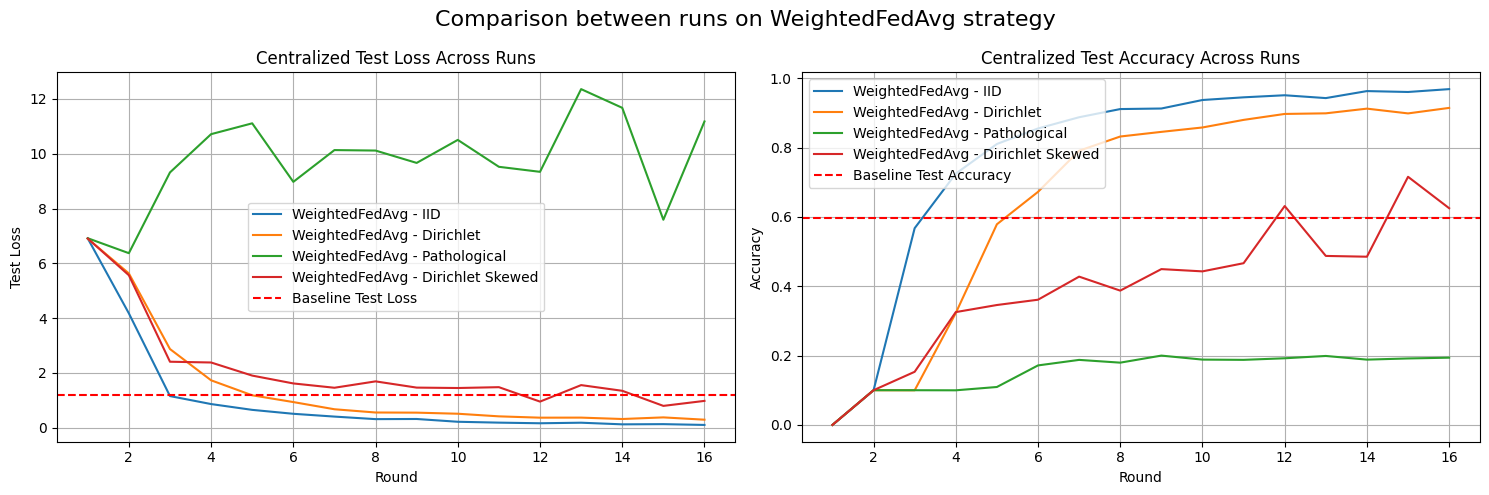
\includegraphics[width=1\linewidth]{img/experiment_2/weightedfedavg-comparison}
        \caption{Comparison between various partition strategy on Weighted-FedAvg aggregation strategy.}
        \label{fig:exp2-weightedfedavg-comparison}
    \end{figure}

    \subsubsection{Summary Table}

    In the Table \ref{tab:experiment_2_results}, the results after the training for each simulation are shown. The rounds to converge was computed as the approximate number of steps to reach a plateau in the test accuracies.

    \begin{table}[h!]
        \centering
        \caption{Test Results for Different Models and Data Partitions in Experiment 2}
        \label{tab:experiment_2_results}
        \begin{tabular}{|l|l|c|c|c|}
            \hline
            \textbf{Model}  & \textbf{Partition}    & \textbf{Test Loss} & \textbf{Test Accuracy} & \textbf{Rounds to Converge} \\
            \hline
            FedAvg          & IID                   & 0.0348             & 99.22\%                & 10                          \\
            FedOpt (Adam)   & IID                   & 3.7302             & 44.14\%                & -                           \\
            Weighted FedAvg & IID                   & 0.9913             & 96.88\%                & 12                          \\
            \hline
            FedAvg          & Dirichlet (alpha=0.5) & 0.1540             & 95.00\%                & 14                          \\
            FedOpt (Adam)   & Dirichlet (alpha=0.5) & 1.7433             & 55.82\%                & -                           \\
            Weighted FedAvg & Dirichlet (alpha=0.5) & 0.2904             & 91.46\%                & 11                          \\
            \hline
            FedAvg          & Pathological          & 6.2423             & 20.22\%                & 11                          \\
            FedOpt (Adam)   & Pathological          & 6.7886             & 16.99\%                & 12                          \\
            Weighted FedAvg & Pathological          & 6.3691             & 19.40\%                & 6                           \\
            \hline
            FedAvg          & Dirichlet (alpha=0.1) & 0.6258             & 78.78\%                & 14                          \\
            FedOpt (Adam)   & Dirichlet (alpha=0.1) & 1.9128             & 41.53\%                & -                           \\
            Weighted FedAvg & Dirichlet (alpha=0.1) & 0.7943             & 71.58\%                & -                           \\
            \hline
        \end{tabular}
    \end{table}


    \section{Discussion}

    This section discusses the key findings from both experiments, emphasizing the implications of federated optimization strategies and data partitioning schemes on convergence behavior and model performance.

    \subsection{Effect of Optimization Strategies in Experiment 1}

    In the Equal Hardware Experiment, all clients possessed identical computational capacity and participated at a fixed fraction (0.3) each round. Under this controlled setting, we compared FedAvg against several FedOpt variants (AdaGrad, Adam, Yogi) across three partitioning scenarios (IID, Square, Dirichlet). The main observations are:

    \begin{itemize}
        \item Under IID Partitioning (Section \ref{subsubsec:iid-scenario}), all strategies eventually converged to very similar final accuracy ($-0.92$), but they differed in convergence speed:
        \begin{itemize}
            \item FedOpt with Yogi converged fastest, reaching a stable plateau by round 24, whereas FedAvg required 47 rounds and both AdaGrad/Adam variants needed 40 rounds (Table 1).
            \item Although final accuracies were nearly identical, FedOpt (Yogi) exhibited smoother validation‐loss curves with fewer oscillations, suggesting that its adaptivity helps dampen fluctuations when data are identically distributed.
        \end{itemize}
        \item In the Square Partitioning setup (Section \ref{subsubsec:square-scenario}), where sample sizes per client grew quadratically, we observed that:
        \begin{itemize}
            \item FedAvg itself achieved a respectable 90.2\% final accuracy but failed to formally “converge” within the 50‐round window (denoted as N/A in rounds to converge).
            \item Among FedOpt variants, Adam yielded the highest final accuracy (91.8\%) in 39 rounds. Both AdaGrad and Yogi matched each other at 91.6\% and converged in 38 rounds (Table \ref{tab:square_performance}).
            \item The fact that all FedOpt variants outperformed FedAvg under strong data‐quantity imbalance (Square) indicates that server‐side adaptivity can compensate for uneven local contributions, but Adam’s slightly higher accuracy suggests it better balances large‐ versus small‐client updates in this scenario.
        \end{itemize}
        \item Dirichlet Partitioning (Section \ref{subsubsec:dirichlet-scenario}) introduced both sample‐size and label‐distribution heterogeneity. Here:
        \begin{itemize}
            \item FedAvg struggled, achieving only 79.6\% accuracy with a high final loss (1.84) and no clear convergence.
            \item FedOpt (AdaGrad) outperformed all, reaching 87.9\% accuracy with a relatively low final loss (0.42) after 41 rounds. FedOpt (Adam) trailed slightly at 86.5\% with a higher loss (0.87) in 40 rounds, and FedOpt (Yogi) matched FedAvg’s 79.6\% but required even more rounds (43).
            \item These results highlight that adaptive methods are critical under statistical heterogeneity. AdaGrad’s per‐parameter learning‐rate scaling seems particularly robust to non‐IID label skews, whereas Yogi’s performance fell off sharply—suggesting its momentum or correction terms may be ill-suited to extreme class‐imbalance in this setting.
        \end{itemize}
    \end{itemize}

    \subsection{Impact of Partitioning Strategies in Experiment 1}
    By holding optimizer choice constant and varying data partitions, Experiment 1 clarifies how data heterogeneity alone influences federated training when hardware is equal:

    \begin{itemize}
        \item IID Partitioning represents the “best‐case” scenario, where all clients see identically distributed samples. Under IID, all methods (FedAvg and FedOpt variants) converged to high accuracy ($-0.92$), with minimal variance in validation trajectories. This confirms that when data are balanced, federated gaps versus centralized training are small.
        \item Square Partitioning, which creates extreme sample‐count heterogeneity, exposed FedAvg’s slower convergence—in spite of identical local compute—because small‐sample clients contributed much noisier gradients. FedOpt variants (especially Adam) mitigated this by re‐weighting updates so that large‐sample clients do not overwhelm smaller ones entirely. Hence, while FedAvg attained strong baseline accuracy (90.2\%), FedOpt’s adaptivity delivered a modest $-1.6\%$ boost (91.8\%).
        \item Dirichlet Partitioning—our most realistic simulation of non‐IID label distributions—had the largest overall performance drop. FedAvg collapsed to under 80\% accuracy, indicating that naive averaging across clients with divergent class labels causes severe model drift. In contrast, FedOpt (AdaGrad) recovered nearly 88\%, showing that adaptive learning rates per update effectively correct for client‐level class skews. This suggests that in any real‐world FL deployment where clients naturally observe different label frequencies, adaptive strategies are essential just to approach baseline accuracy.
    \end{itemize}

    Taken together, Experiment 1 underscores that partitioning strategy alone can shift final test accuracy by over 15 percentage points (from 92\% down to 79\%), and that adaptive optimizers can recover much of this loss.

    \subsection{Effect of Optimization Strategies in Experiment 2}

    From the first experiments, the choice of optimization strategy had a substantial impact on model performance and convergence speed.

    \textbf{FedAvg} consistently provided a reliable baseline across all partitioning schemes. It showed strong performance under IID conditions and was more stable than FedOpt in the full participation setup. However, its convergence was relatively slower, particularly in non-IID scenarios like Dirichlet and Pathological.

    \textbf{FedOpt} exhibited a high degree of sensitivity to data heterogeneity. In this experiment, it often failed to converge or converged to poor solutions, especially under full participation with heterogeneous clients. This may be due to choosing only the Adam variant of this strategy, but it can also suggest that while adaptive optimizers can accelerate training, they are also more prone to instability when exposed to system-level variability or extreme data imbalance.

    \textbf{Weighted FedAvg}, which incorporates both the number of samples and the number of epochs trained per client, proved effective in full-participation scenarios. It consistently achieved near-baseline accuracy, especially in IID and Dirichlet setups, and demonstrated the fastest convergence in the Pathological scenario. These results suggest that weighting updates not just by data volume but also by compute effort helps stabilize training in heterogeneous federated environments.

    \subsection{Impact of Partitioning Strategies in Experiment 2}

    The partitioning strategy had a significant influence on learning dynamics:

    \begin{itemize}
        \item \textbf{IID partitions} enabled the fastest and most stable convergence across all algorithms. Models reached near-centralized performance levels with minimal rounds, especially with FedAvg and Weighted FedAvg.

        \item \textbf{Dirichlet partitions ($\alpha = 0.5$ and $0.1$)} introduced class imbalance and led to slower convergence and reduced accuracy. Still, Weighted FedAvg mitigated this effect better than FedAvg or FedOpt, suggesting that accounting for local effort in aggregation can improve robustness to statistical heterogeneity.

        \item \textbf{Pathological partitions}, where clients had access to only a subset of classes, posed the greatest challenge. All algorithms experienced sharp drops in accuracy and required more rounds to converge, with FedOpt (Adam) often underperforming due to poor generalization.
    \end{itemize}

    \subsection{Convergence Behavior and System Implications in Experiment 2}

    We observed notable differences in how quickly and reliably each strategy converged under various conditions. FedAvg and Weighted FedAvg generally converged within 10–15 rounds in stable scenarios. In contrast, FedOpt showed delayed or unstable convergence, particularly when exposed to asynchronous or variable client training durations in Experiment 2.

    The full participation setup revealed that while involving all clients each round maximizes resource utilization, it also increases the risk of synchronization issues due to heterogeneity in local computation time. Our simulation using different epoch distributions (\(\mathcal{N}(5,1)\), \(\mathcal{N}(10,1)\), and \(\mathcal{N}(15,1)\)) effectively demonstrated the semi-asynchronous behavior of real-world federated systems.

    \subsubsection{Recommandations}
    Based on our two experiments:

    \begin{itemize}
        \item \textbf{Assess Data Heterogeneity Early}: Profile client data distributions (sample counts, class frequencies) before choosing an algorithm. If non‐IID effects are minor, FedOpt (AdaGrad or Yogi) can accelerate training. If severe, consider robust weighting schemes.
        \item \textbf{Choose Adaptive Federated Optimization Sparingly}: Use FedOpt only when clients synchronize on a fixed local‐epoch schedule. If clients cannot be forced to train the same number of epochs, adaptive optimizers like Adam may introduce instability.
        \item \textbf{Implement Effort‐Aware Aggregation for Full Participation}: In any setting where clients train asynchronously or at variable speeds, track both sample count and local‐training effort. Weighted averaging based on (samples $\times$ epochs) helps mitigate stale or overly aggressive updates.
        \item \textbf{Balance Participation Fraction}: Requiring every client every round maximizes data usage but introduces straggler risk. A moderate fraction (e.g., 0.3 as in Experiment 1) can yield near‐optimal accuracy while avoiding severe synchronization stalls.
    \end{itemize}


    \section{Conclusions \& Future Work}
    Our two experiments revealed that data heterogeneity is the primary driver of performance loss in federated learning. Under equal‐hardware partial participation (Section \ref{subsec:experiment1}), adaptive optimizers (AdaGrad, Adam, Yogi) outperformed FedAvg when data were imbalanced or labels skewed, with AdaGrad most robust under extreme Dirichlet splits and Adam excelling under sample‐count imbalance. However, when all clients participated with variable local epochs (Section \ref{subsec:experiment2}), these adaptive methods (especially Adam) became unstable, often failing to converge. Instead, Weighted FedAvg, which scales updates by (samples $\times$ epochs), offered the best trade‐off of convergence speed and final accuracy in semi-asynchronous settings. In both regimes, no single method was universally optimal.

    Some future work points would be:
    \begin{itemize}
        \item \textbf{Dynamic Client Scheduling}. Investigate participation schemes that adaptively include or exclude clients based on data skew, resource constraints, or recent contributions to mitigate straggler delays.
        \item \textbf{Joint Feature -- Label Heterogeneity}. Extend simulations to incorporate both feature and label non‐IID splits, assessing whether new correction terms or optimizer tweaks can better handle complex skews.
        \item \textbf{Extended Training for FedOpt in Experiment 2}: Increase the number of global rounds and local‐epoch budgets when using adaptive optimizers (e.g., Adam, AdaGrad) under full participation to determine if longer training stabilizes their moment estimates and closes the accuracy gap observed in Experiment 1.
        \item \textbf{Hyperparameter Tuning under Variable Epochs}: Systematically explore learning‐rate schedules, momentum decay, and adaptive‐optimizer coefficients when clients train for different epoch counts, to identify configurations that mitigate instability in semi-asynchronous settings.
        \item \textbf{Hybrid Aggregation Strategies}: Combine elements of FedOpt (e.g., per‐parameter learning‐rate adjustments) with (samples $\times$ epochs) weighting to see if a mixed approach recovers FedOpt’s convergence speed from Experiment 1 while retaining the stability of Weighted FedAvg in Experiment 2.
    \end{itemize}

    By addressing these areas, future federated‐learning systems can better balance accuracy, communication efficiency, and robustness to real‐world heterogeneity.

    \bibliographystyle{alpha}
    \bibliography{biblio}

\end{document}